% This is a LaTeX version of the sample laboratory report
% from Virginia Tech's copyrighted 08-09 CHEM 1045/1046 lab manual.
% Reproduction of this one appendix section for educational purposes
% should fall under fair use.

\documentclass{article}
\usepackage{enumerate}
\usepackage{graphicx}
\usepackage{wrapfig}
\usepackage{float}
\usepackage[margin=1in]{geometry}
\usepackage{subcaption}
\usepackage{amsmath}

\providecommand{\e}[1]{\ensuremath{\times 10^{#1}}}

\graphicspath{{img/}{./img/}}

\title{Wavefront Aberation Analysis Lab Report \\
VS212A - Optics \& Dioptrics of the Eye}
\author{Vasha DuTell}

\begin{document}

\maketitle

\begin{tabular}{lr}
\end{tabular}

\section{Introduction}
This is a lab report documenting the analysis of wavefront abberation data collected from a Shack-Hartmann wavefront sensor, for 17 students in the Fall 2015 VS212A class. This report details the methods for data collection, results of data analysis, and discussion of the results, as well as 3 eye optics exercises. \\

\section{Methods}

\subsection{Measurement Conditions}

\subsubsection{Subjects \& Data Collection} 17 students were measured by Austin, each the right eye only, in order of their volunteering, and all on the same Shack-Hartman wavefront sensor. The headrest and chinrest was thoroughly cleaned with alcohol wipes by Jazzi in between each student. Pupils measured were natural, not dilated or frozen to stop accommodation. This is an important note, as any accommodation that might have been occurring, is indistinguishable from myopia, and therefore may affect the value of the second order Zernike coefficient corresponding to defocus ($Z_0^2$). Each student was measured 4-5 times, and the best resulting image was hand-chosen by Austin. A few individuals students were measured for repeatably between trials, and the results were found to be repeatable. Austin then used these images to calculate the corresponding Zernike Polynomial coefficients for each student.\\


\subsubsection{Lighting Conditions} Lighting conditions were mesopic, or slightly lit, with the room lights were turned off, and a little ambient light, just a few computer screens and cracked doors. The majority of the light in the room was from a cracked door behind the wavefront sensor, to which the subjects faced. This door was completely shut during the measurement of the later-measured students. \\

\subsubsection{Adjustments for Refractive Error} For students with a strong refractive error, the sensor was adjusted to make a smaller pinhole light source, in order to decrease refraction and allow for an analyzable image, but at the expense of total light. In the case of one student, defocus error was strong enough that an on-glasses measurement was used. In the case of another student who was already wearing contacts, the lenses were left on. \\

\subsection{The Shack-Hartmann Wavefront Sensor}
The Shack-Hartmann Wavefront Sensor is an optical instrument used to measure the incoming wavefront from an optical system. Specifically, it is used to detect any aberrations in the incident wavefront. \\

The sensor is named after Johannes Franz Hartmann, and Roland Shack, two scientists who made significant contributions to its design. The preliminary work was done by Johannes Franz Hartmann, who designed the first aperture array in 1900 for ray tracing in a telescope\cite{hartmann1900}. The apterature array, also known as a Hartmann screen, consisted of small holes placed in a regular pattern over a solid screen. In 1971, Roland Shack added small lenses inside the aperatures, creating the first full wavefront sensor \cite{shack71}.\\

\begin{figure}[h]
  \centering
    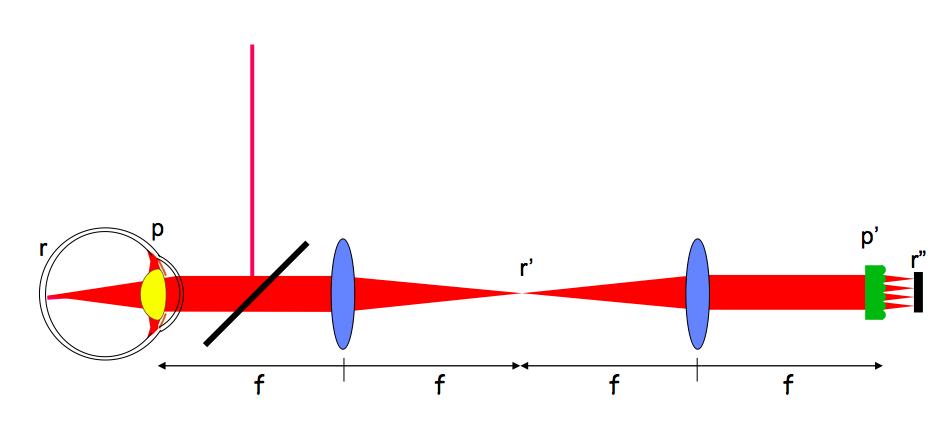
\includegraphics[width=.75\linewidth]{shwfs.png}
  \caption{Shack-Hartmann Wavefront Sensor Diagram.(reprinted from{\cite{austinsslides}}).}
  \label{fig:shwfs}
\end{figure}

Figure \ref{fig:shwfs} shows a diagram of the sensor. Design of the sensor is as follows: A light point source enters the optical system by means of a partially reflective mirror. Light travels from this mirror into the optical system of interest, in our case the eye, where it is reflected back onto the retina, and back through the eye's lens. Any aberrations from the eye are now present in the wavefront, and travel marginally undisturbed through the system. A portion of this light from the eye then passes through the partially reflective mirror, to a set of two lenses, where it is focused to a point, inverted, (also magnified?), and focused at infinity in preparation for transmission to the lenslet array. It then passes through the lenslet array, comprised of many tiny lenses arranged in a grid pattern, and projected onto a CCD camera, where the image is captured.

\begin{wrapfigure}{r}{0.4\linewidth}
  \centering
    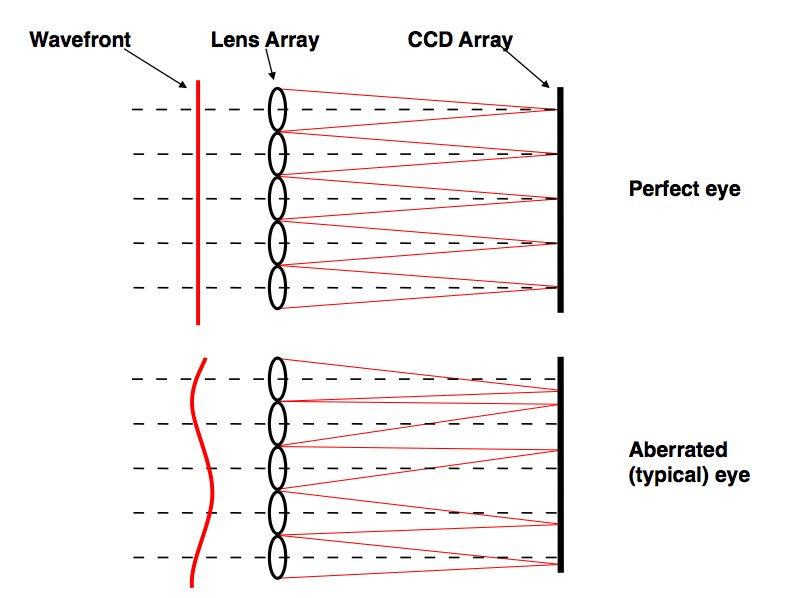
\includegraphics[width=1\linewidth]{wavefrontabb.png}
  \caption{Wavefront Abberation in ideal and typical eye.(reprinted from{\cite{austinsslides}}).}
  \label{fig:wfabb}
\end{wrapfigure}

\begin{wrapfigure}{r}{0.25\linewidth}
  \centering
    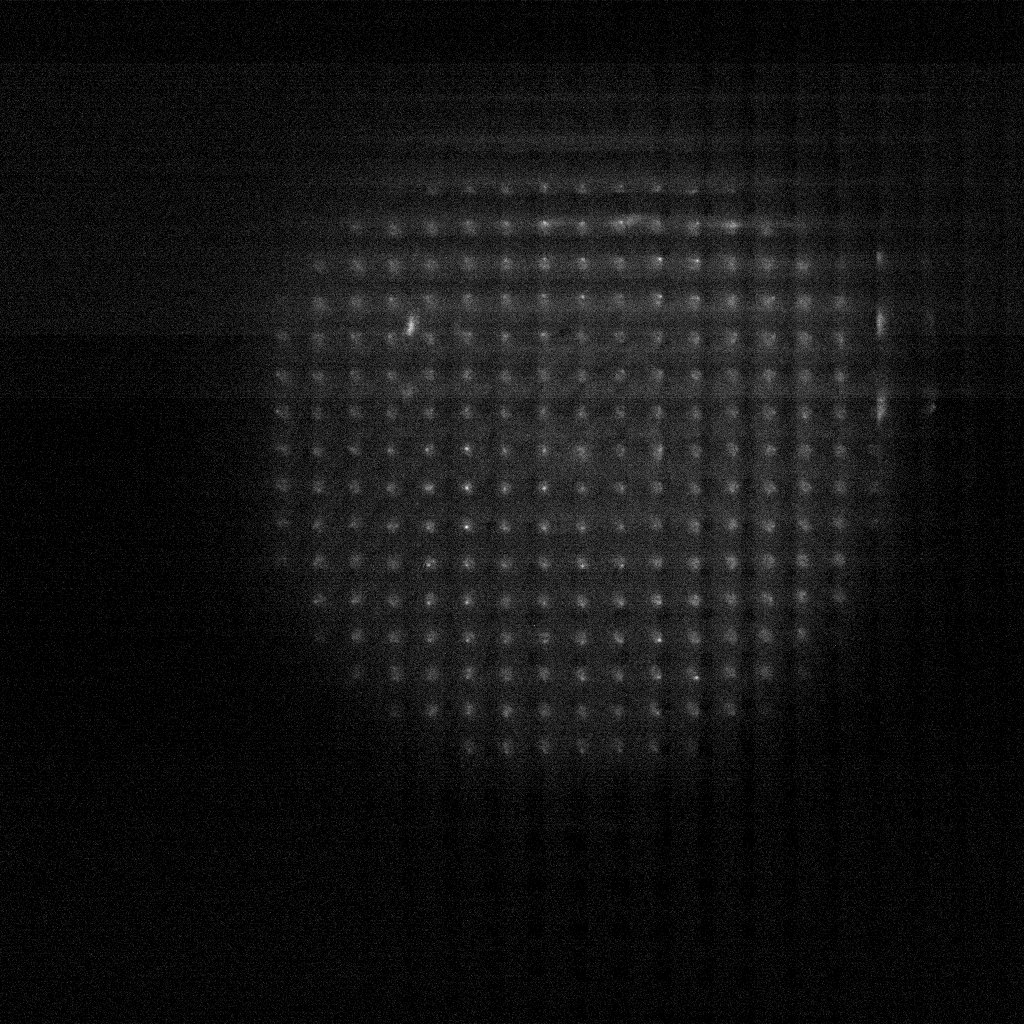
\includegraphics[width=1\linewidth]{Vasha_R_G_0530_2.png}
  \caption{Image of Vasha's Wavefront}
  \label{fig:wfvasha}
\end{wrapfigure}

The lenslet array is the key piece of the sensor. Each lens detects an individual portion of the wavefront \ref{fig:wfabb}. In a perfect eye, the wavefront is perfectly normal to the front of the array, and therefore hits the same spot on every lens in the array. Each lens in the array the projects the wavefront through at the same angle, resulting in a perfect grid pattern of points projected onto the CCD. In the typical eye that contains aberration, the wavefront coming from the eye is curved, not normal to the front of the array, and therefore hits each lenslet in the array at a different angle. This causes the lenslets to project a non-uniform grid pattern to the CCD for imaging.  An example of a photo taken by the CCD is in Figure \ref{fig:wfvasha}. \


 Each type of abberation in the wavefront causes a different imprefection in the grid-like pattern, and because the geometry of the lenslet array and its relationship to the CCD camera is known, the shape of the wavefront can be reconstructed from the grid-like pattern of points imaged. This wavefront shape can be described by a sum of Zernike polynomials.\
 
\subsection{Zernike Polynomials}

\begin{wrapfigure}{r}{0.3\linewidth}
  \centering
    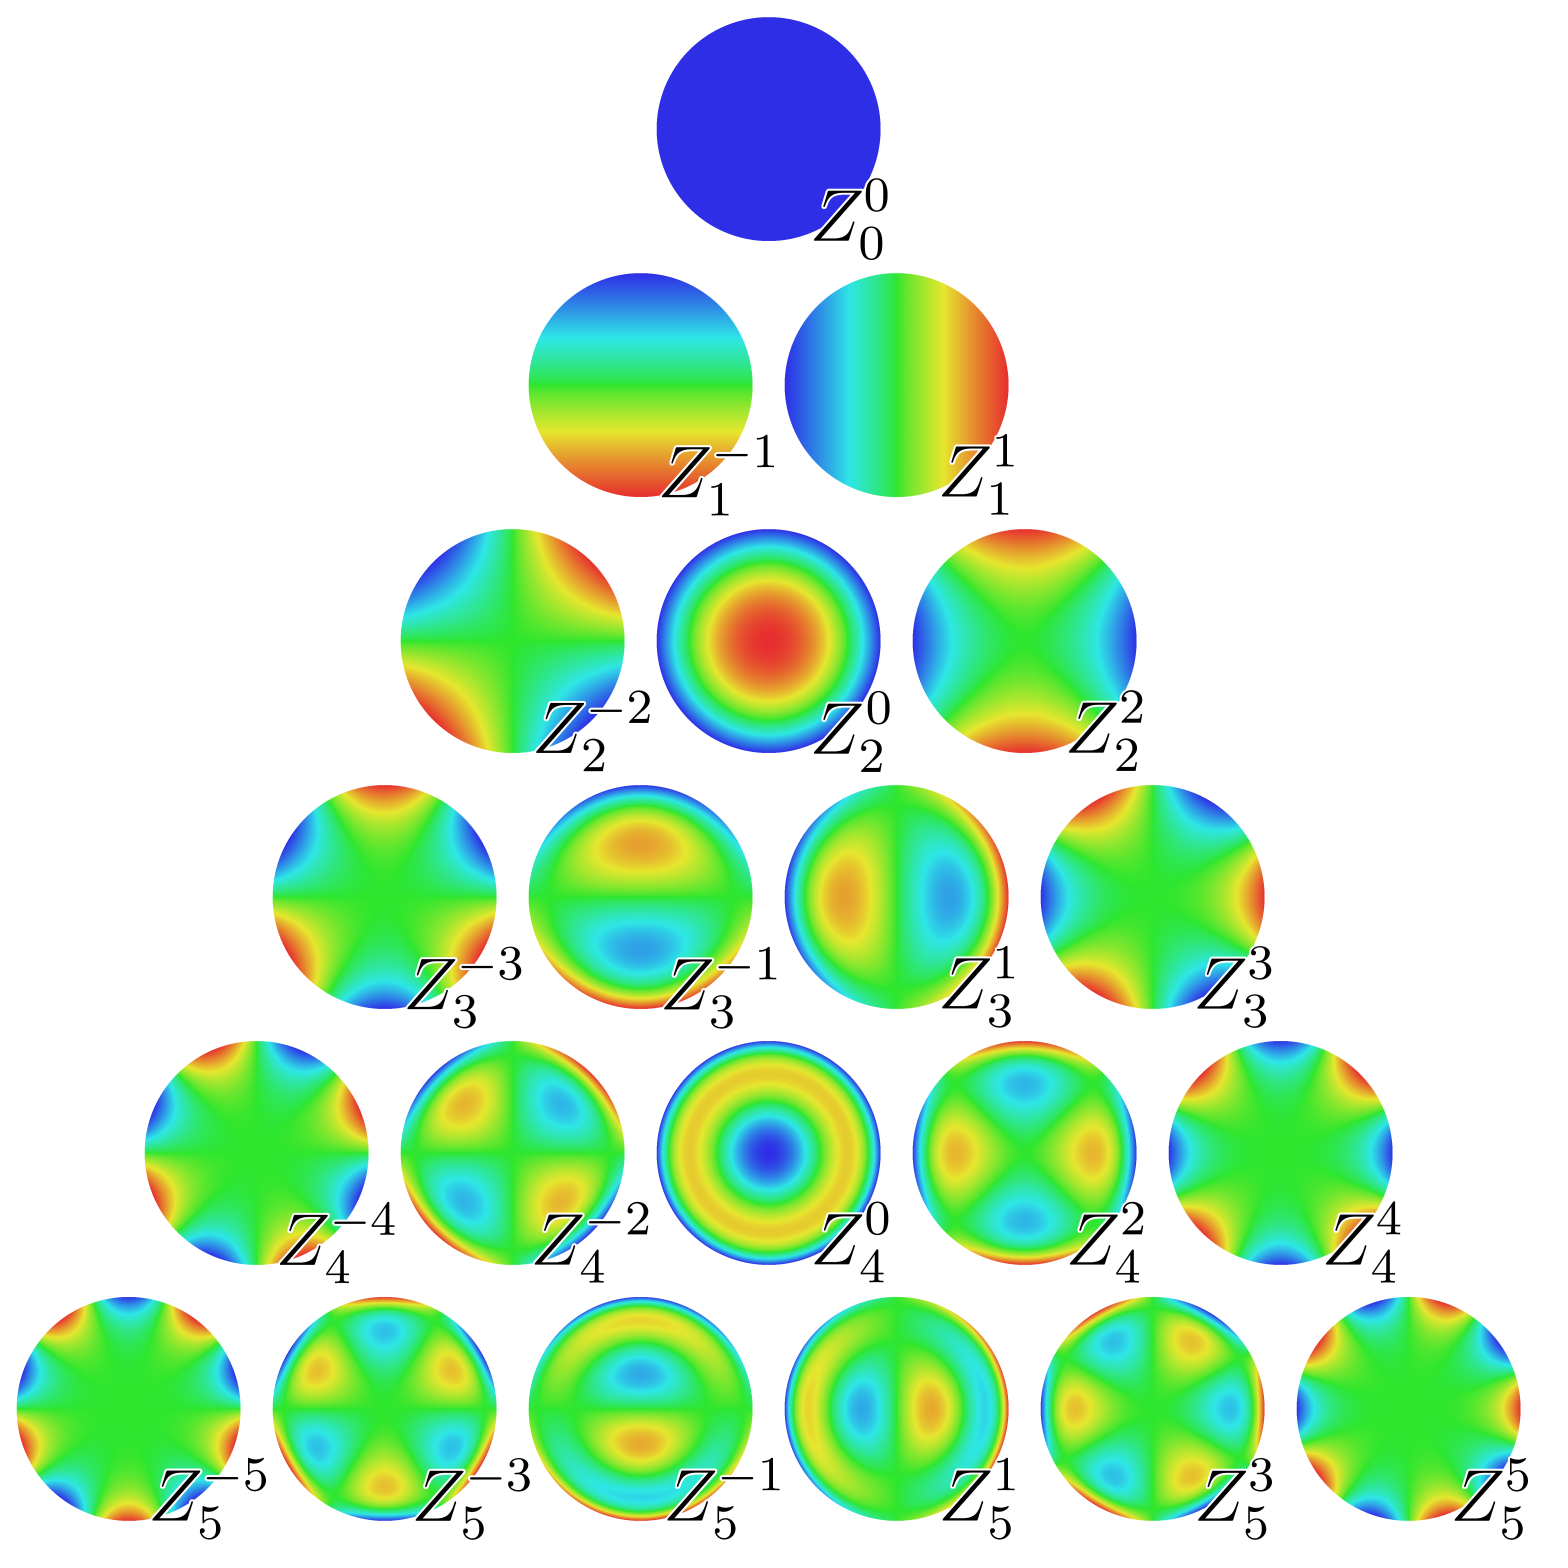
\includegraphics[width=1\linewidth]{Zernike_polynomials2.png}
  \caption{Zernike Polynomials(reprinted from Wikipedia).}
  \label{fig:zps}
\end{wrapfigure}


\begin{table}[htbp]
	\centering
	\begin{tabular}{ccc}
	& Zernike Term	Name \\ \hline
	$Z^0_0$	&	Piston \\
	$Z^1_1 Z^{-1}_1$	&	Tilt (Prism) \\
	$Z^0_2$	&	Defocus \\
	$Z^2_2, Z^{-2}_2$	&	Astigmatism \\
	$Z^2_4, Z^{-2}_4$	&	Secondary Astigmatism \\
	$Z^0_4$	&	Spherical Aberration \\
	$Z^1_3,Z^{-1}_3$	&	Coma \\
	$Z^3_3, Z^{-3}_3$	&	Trefoil \\
	$Z^4_4, Z^{-4}_4$	&	Quadrafoil \\
    \end{tabular}
      \caption{Zernike Polynomials(reprinted from Wikipedia).}
      \label{table:Low Order ZPs }
\end{table}

Zernike polynomails (ZPs) are a mathematical means of describing abberations to a wavefront. Each polynomial describes a different abberation shape, and these shapes can be pieced together with different weights to perfectly describe any given wavefront. The Zernike polynomials are: orthagonal, normalized, and efficient in describing occular wavefront abberations, in that the shapes are similar to what is found in the eye, and the lowest order polynomials the most common. The first few are shown in Figure \ref{fig:zps}. \


An Zernike equation for a given wavefront aberration is formulated by calculating for each polynomial, the coefficient by which that polynomial is multiplied, therefore describing the magnitude to which each given polynomial contributes to the full equation. Because the polynomials are all orthogonal, we can calculate these coefficients independently, as the value one does not affect the value of any other. \

\subsection {Data Summary Table}

\begin{center}
 \begin{tabular}{||c c c c||} 
 \hline
 Student & Has refractive error? & Wearing Contacts/Glasses? & Pupil Sizes Measured\\ [0.5ex] 
 \hline\hline
 Angie & No & No & 300,400,500,600,700,744 \\ 
 \hline
 Bala & Yes & No & 300,400,469 \\ 
 \hline
 Baldwin & No & No & 300,400,500,600,675 \\ 
 \hline
 Bensaid & No & No & 300,400,500,600,700,759 \\ 
 \hline
 Billie & No & No & 300,400,500,600,678 \\ 
 \hline
 Ethan & No & No & 300,400,500,600,697 \\ 
\hline
 Jazzi & Yes & No & 300,400,500,600 \\ 
\hline
 Kat & Yes & Contacts & 300,400,500,600,700,765 \\ 
 \hline
 Linyue & Yes & No & 300,400,500,600,700,725 \\ 
 \hline
 Liz & Yes & No & 300,400,500,600,636 \\ 
 \hline
 Michael & Yes & No & 300,400,500,538 \\ 
 \hline
 Natalie & Yes & Glasses & 300,400,500,562 \\ 
 \hline
 Peter & Yes & No & 300,400,500,577 \\ 
 \hline
 Sanam & No & No & 300,400,500,600,638 \\ 
 \hline
 Sarah & Yes & No & 300,400,500,600,625 \\ 
 \hline
 Sylvain & No & No & 300,400,500,600,700,800,801 \\ 
 \hline
 Vasha & Yes & No & 300,400,500,600,631 \\ 
 \hline
 \hline
\end{tabular}
\end{center}

\begin{tabular}{ll}
Total number of students measured & 17 \\
Total number of students with refractive error & 10 \\
Total number of students wearing glasses & 1 \\
Total umber of students wearing contacts & 1 \\
\end{tabular}


\section{Results}

\subsection{16 Sets of ZPs over 5mm Pupil}

\subsubsection{Summary Statistics}
Summary statistics for the 16 sets of Zernike coefficients that were calculated for a 5 mm pupil are as follows:

Mean

\begin{figure}[h]
  \centering
    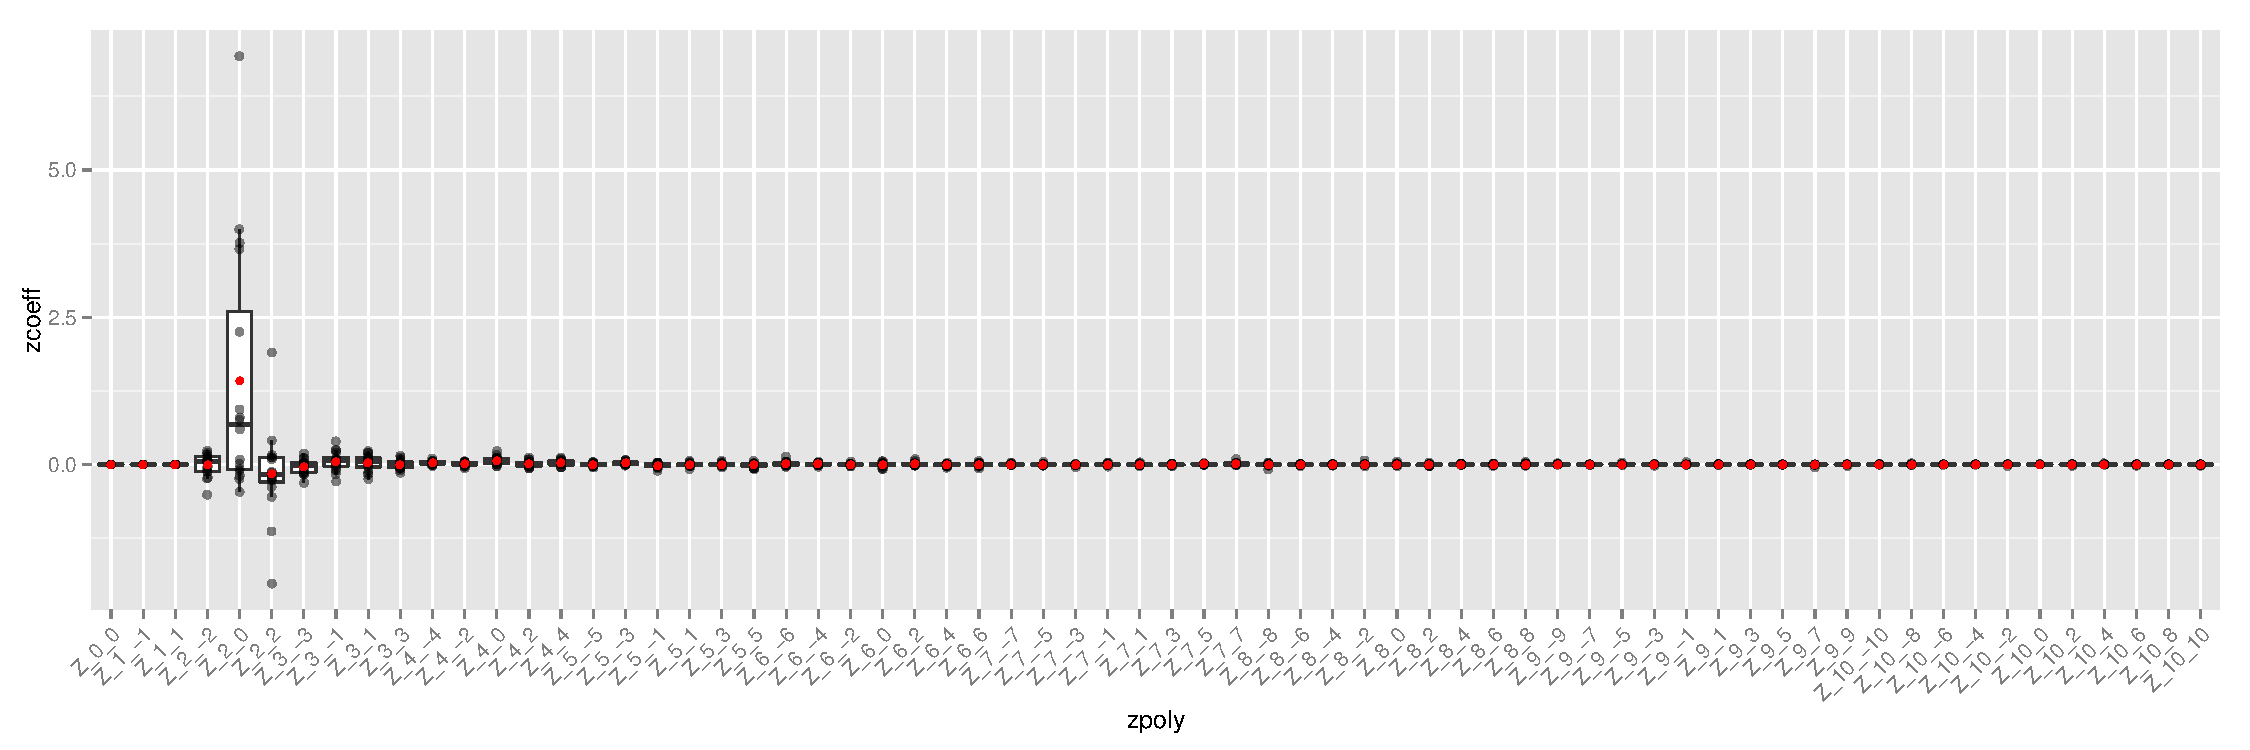
\includegraphics[width=1\textwidth]{meanbar.pdf}
  \caption{Coefficient values for each of the 63 Zernike polynomials. Red: mean.}
  \label{fig:meanbar}
\end{figure}

The mean values in Figure \ref{fig:meanbar}, and plotted in red, for coefficients corresponding to each of the Z. polynomials are around zero for almost all polynomials, except for $Z_2^0$, which corresponds to defocus. The coefficient for this polynomial was high in the case of a few students, particularly Michael, with a value of 6.93, as well as Vasha, Ethan, and Peter, with values all around 4. I know that I am myopic, and these students are likely also myopic, as although they could have been accommodating to some degree, they likely could not have accommodated this strongly.\ 

In addition to $Z_2^0$, The mean value for the coefficient corresponding to polynomial $Z_2^2$ also deviated from zero, but in this case negatively. This polynomial corresponds to astigmatism. While two students (Liz and Linyue) measured relatively high negative numbers (around -2) that contributed to this mean value below zero, Sarah measured a value around +2.\

Standard Deviation

\begin{figure}[h]
  \centering
    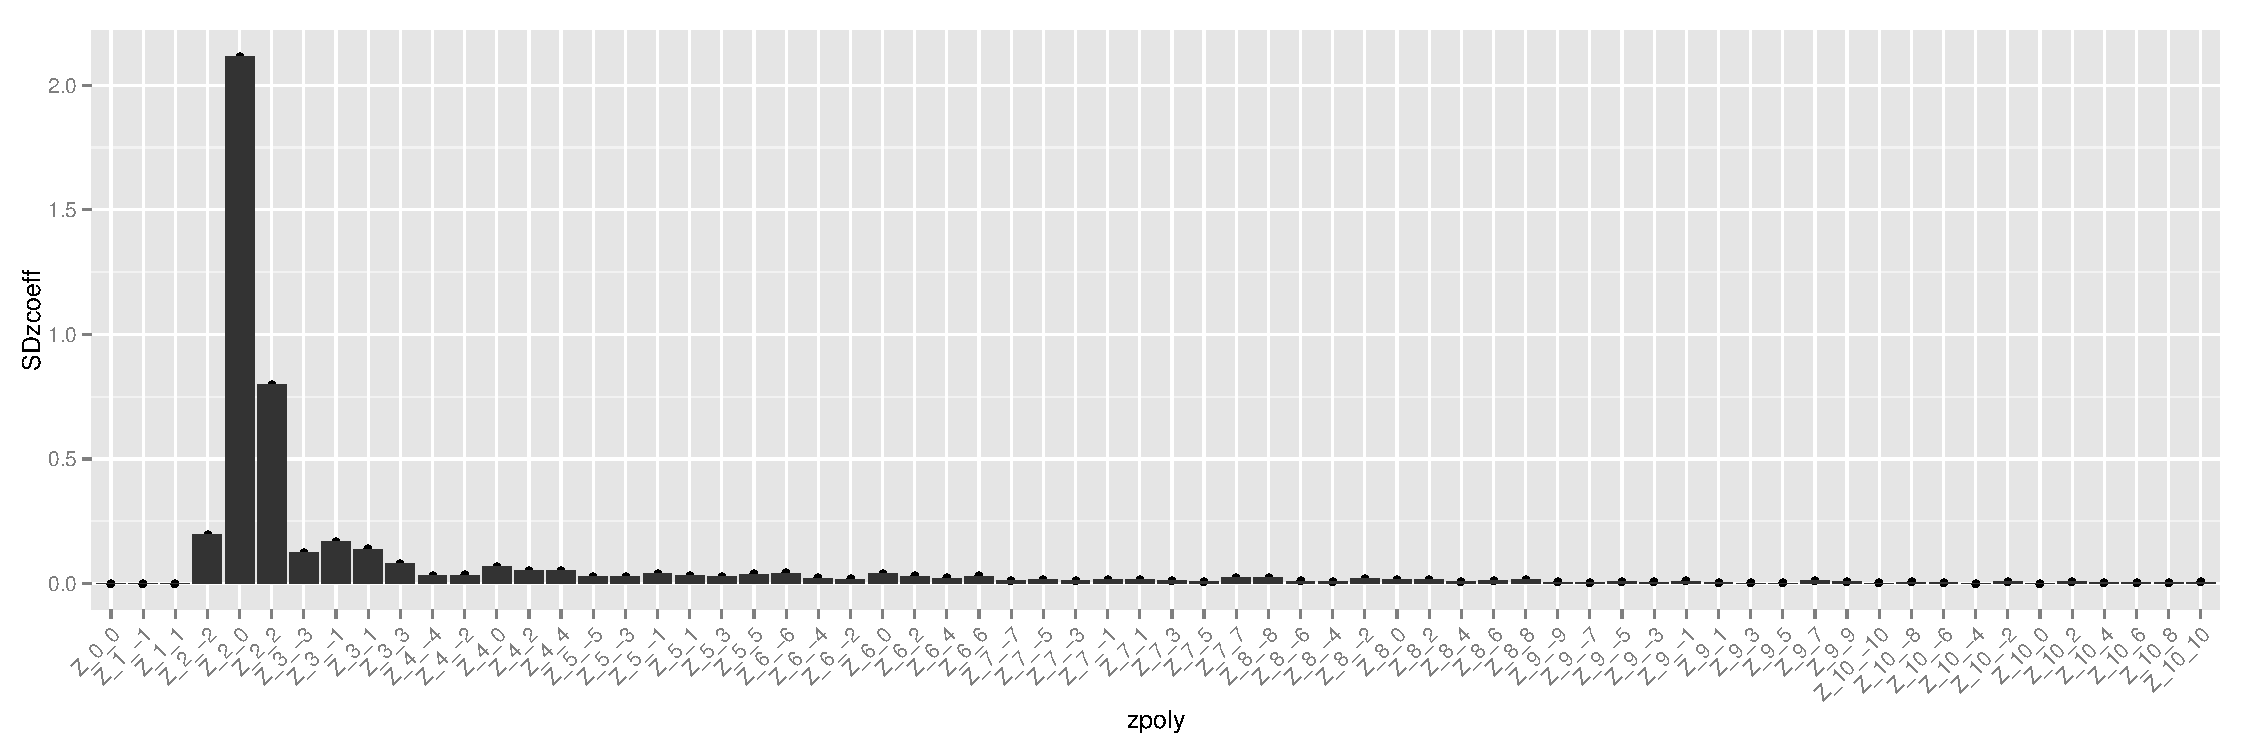
\includegraphics[width=1\textwidth]{stdbar.pdf}
  \caption{Standard Deviation of coefficients values for each of the polynomials.}
  \label{fig:sdbar}
\end{figure}

As could have been inferred from Figure \ref{fig:meanbar}, and made explicit in Figure \ref{fig:sdbar}, the standard deviation of measured values for each of the ZPs is highest for $Z_2^0$, and second highest for $Z_2^2$. Interestingly, the other polynomials nearby show some deviation about their values, particularly other 2nd and 3rd-order ZPs: $Z_2^{-2}$, $Z_3^{-3}$, $Z_3^{-1}$, $Z_3^1$, and $Z_3^3$, even though their mean values were very near zero. $Z_4^0$ may also show a small deviation above zero, but this distance quickly trails off into the other 4th and higher order polynomials. This result is not surprising given we know 2nd and 3rd order ZPs describe well the most common eye aberrations in humans.\

\subsubsection{RMS}

The ZPs can be separated into their respective orders, as determined by the first number in their name, and by their level from the top in Figure \ref{fig:zps}. For each order (1-10) we calculate the Root Mean Square (RMS) value as the square root of the sum of squares of all ZPs of that order. 

\begin{figure}[H]
  \centering
    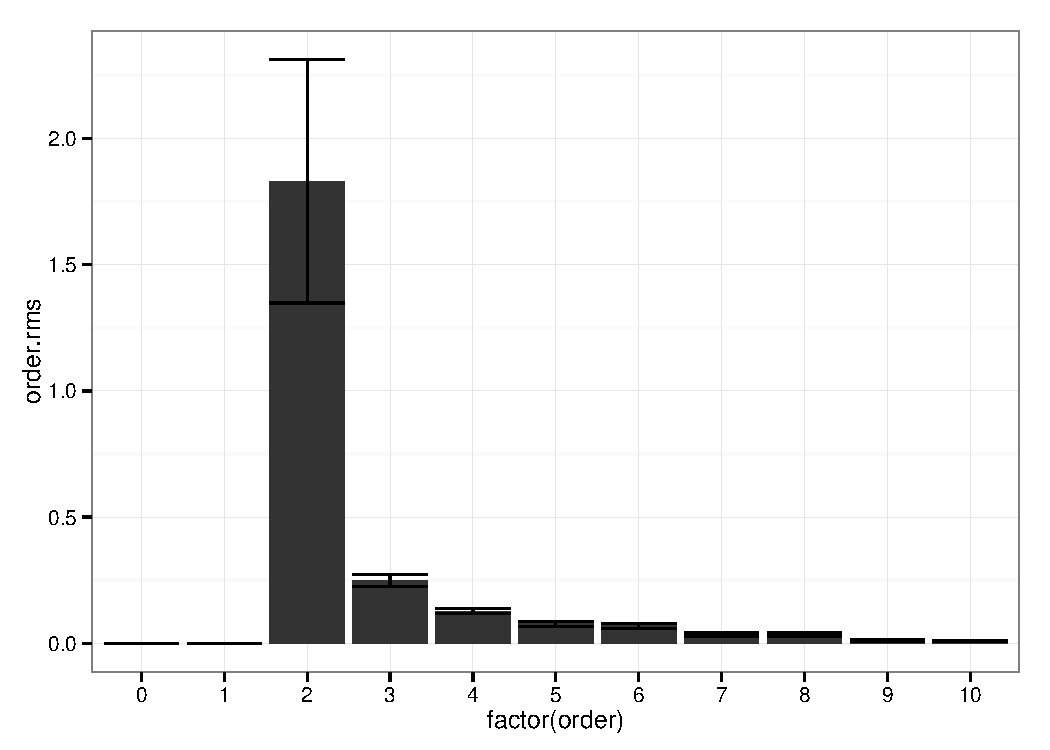
\includegraphics[width=.5\textwidth]{orderrms.pdf}
  \caption{RMS values for each ZP, averaged over subjects}
  \label{fig:rmsbar}
\end{figure}

In Figure \ref{fig:rmsbar}, we see the RMS values for each order, averaged over all students, with standard error included. We see that 2rd order ZPs have high RMS on average around 1.8, but there is also a relatively large SE for these values also, around 0.5. The RMS decreases as the order increases, with orders 3 and 4 and larger with values for RMS less than 0.25, and SE less than 0.1. \

\subsubsection{High Order RMS \& Strehl Ratio}

We can also calculate the High order RMS, one number representing the RMS for all orders 6 and above. We also calculate the Strehl Ratio, a value between 0 and 1, representing the overall quality of image formation, with 1 being perfect image quality. The Strehl ratio is the ratio of the peak intensity of the aberrated image over the maximum possible intensity that would be attained with no aberration. The High Order RMS and the Strehl Ratio for each student are in the table below:

\begin{table}[H]
    \centering
    \begin{tabular}{cccc}
          & High Order RMS & High Order Strehl Ratio & Total Strehl Ratio \\ \hline
        Angie & 0.1777 & 0.1399 & 0.0988 \\
        Baldwin & 0.3546 & 0.0421 & 0.0567 \\
        Bensaid & 0.2903 & 0.0449 & 0.0641 \\
        Billie & 0.2486 & 0.0834 & 0.0172 \\
        Ethan & 0.2501 & 0.0540 & 0.0249 \\
        Jazzi & 0.3641 & 0.0543 & 0.0029 \\
        Kat & 0.3390 & 0.0545 & 0.0373 \\
        Linyue & 0.2151 & 0.0614 & 5$\times10^{-4}$ \\
        Liz & 0.5459 & 0.0454 & 0.0063 \\
        Michael & 0.4091 & 0.0268 & 0.0013 \\
        Natalie & 0.3155 & 0.0605 & 0.0505 \\
        Peter & 0.2686 & 0.0364 & 5$\times10^{-4}$ \\
        Sanam & 0.3691 & 0.0371 & 0.0676 \\
        Sarah & 0.2271 & 0.0610 & 0.0036 \\
        Sylvain & 0.1757 & 0.0918 & 0.0913 \\
        Vasha & 0.4283 & 0.0206 & 4$\times10^{-4}$ \\
    \end{tabular}
\end{table}

High Order RMS (Root Mean Square) represents a value of visual clarity after defocus and astygmatism correction with glasses or contacts. This value then, represents a way to compare the clarty of all students vision given all are corrected to essentially emmetropic vision as corrected by an optomistrist's glasses/contact fitting. A small (close to 0) HO-RMS is an indicator of higher visual accuity, in that the value of higher order aberrations are close to zero. The lowest HO-RMS value in the class is Angie, followed closely by Sylvain. The highest value for HO-RMS in the class is Liz, followed next by Vasha and Michael.

High Order Strehl Ratio represents a value for visual clarity after defocus and astygmatism correction with glasses or contacts. Again, here we can compare across all students after correction such that all are for all clinical purposes emmetropic. A large (close to 1) High Order Strehl Ratio is a better indicator of clear vision (after defocus and astygmatism correction by glasses/contacts) than a low value for High-Order RMS. In comparing the class' vision using this metric, we find Angie to have the highest value, with the next highest value from Sylvain, and followed next by Billie.

Total Strehl Ratio represents a value for visual clarity without correction by glasses or contacts. A large (close to 1) Strehl Ratio is a better indicator of clear vision (before defocus and astygmatism correction by glasses/contacts) than a low-value RMS.  In comparing these values for the class, I have the lowest total Strehl ratio at 4\e{-4}, meaning I have the dimmest maximum PSF intensity before correction, and therefore the poorest vision without correction, with the exception of the student who was measured with their glasses on. Peter and Linyue also had a very similar low Strehl at 5\e{-4}. The highest total Strehl Ratios in the class are Angie and Sylvain. Interestingly, they also represent the best vision as measured by high order strehl ratio, implying the presence of low-order aberrations may be correlated with the presence of higher-order aberrations.

See Discussion section for a comparison of HO-RMS and HO-Strehl as metrics for visual clarity, and their relative ordering of students' values for each metric.

\subsubsection{HO Wave Aberrations \& PSFs}

Now we plot for each subject, the high order wave aberration, and the point spread function at 5mm pupil size:

\begin{figure}[H]
\begin{subfigure}{.5\textwidth}
  \centering
  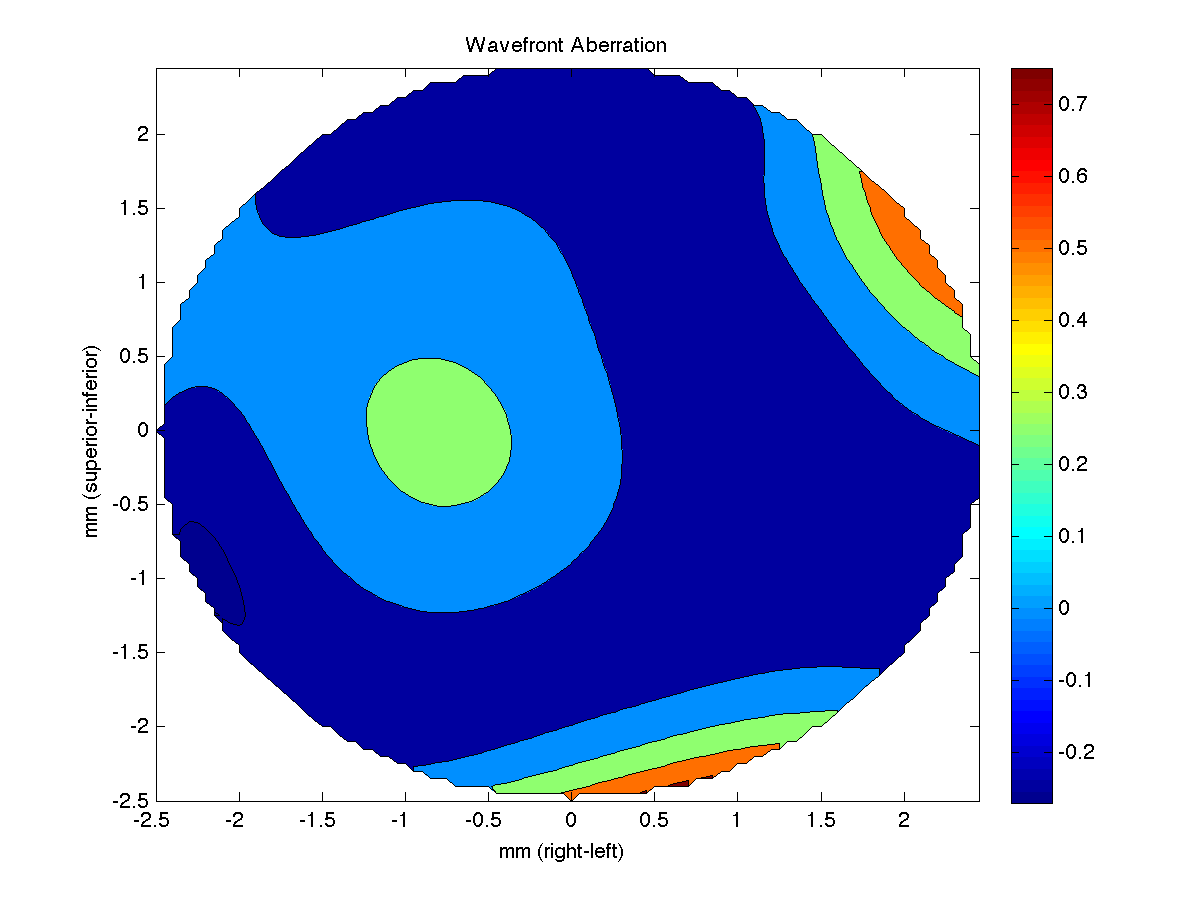
\includegraphics[width=1\linewidth, keepaspectratio]{Angie_WFA.png}
  \caption{High Order Wavefront Aberration}
  \label{fig:angiehowa}
\end{subfigure}%
\begin{subfigure}{.5\textwidth}
  \centering
  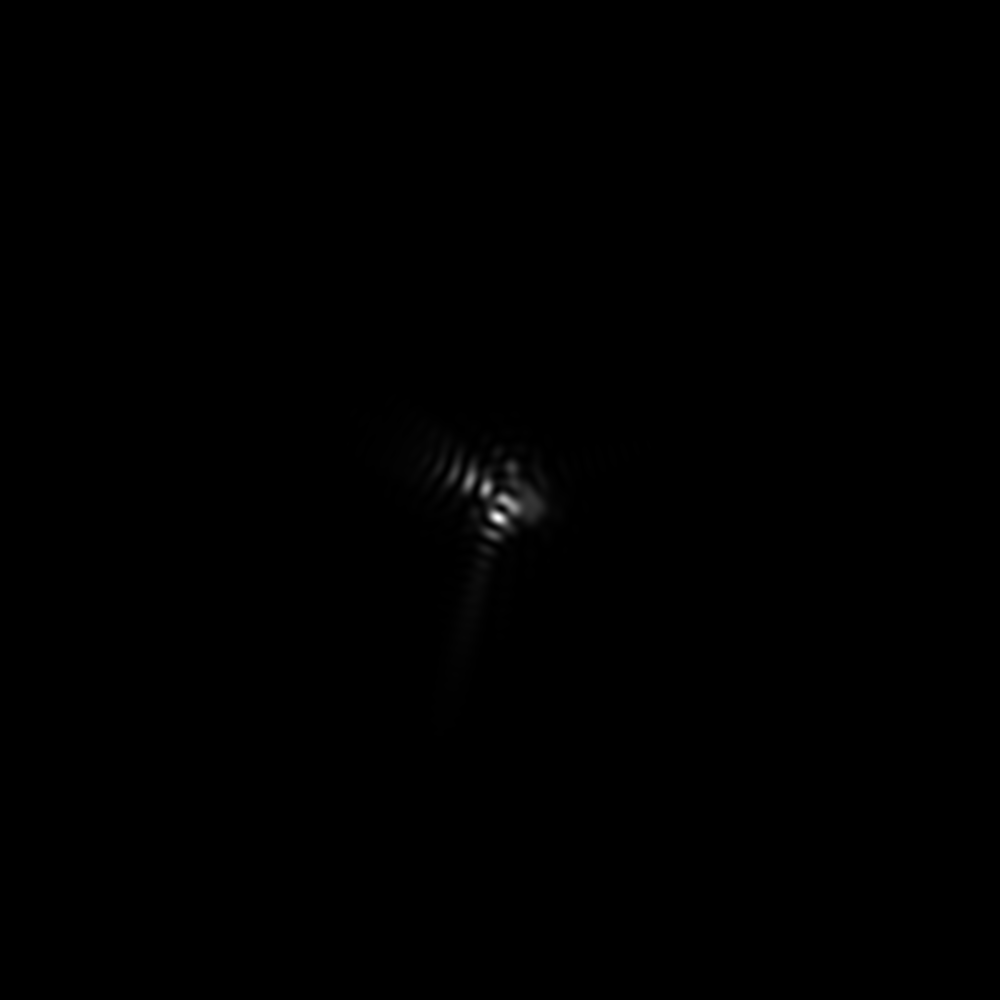
\includegraphics[width=.8\linewidth]{Angie_PSF.png}
  \caption{Point Spread Function}
  \label{fig:angiepsf}
\end{subfigure}
\caption{HO Wave Aberration and PSF for Angie}
\label{fig:angie}
\end{figure}

\begin{figure}[H]
\begin{subfigure}{.5\textwidth}
  \centering
  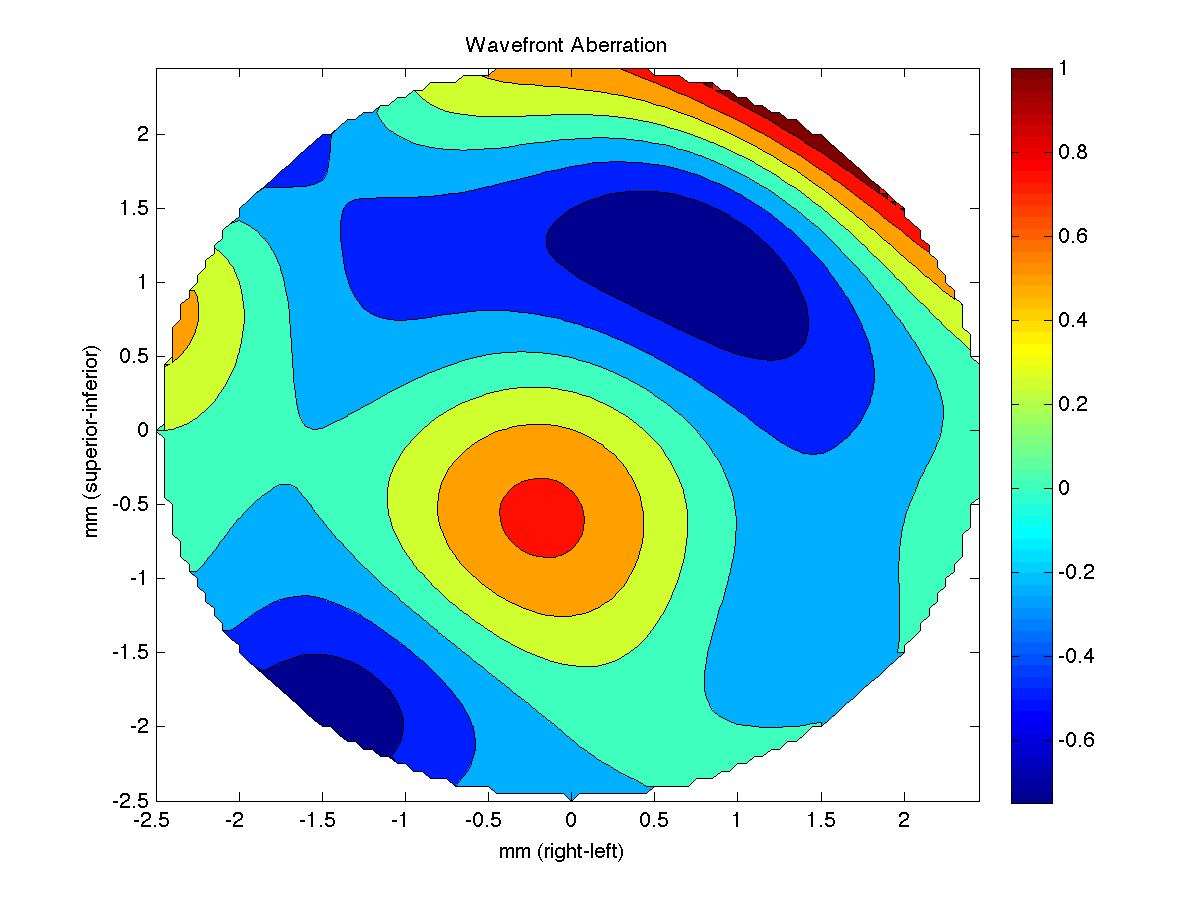
\includegraphics[width=1\linewidth]{Baldwin_WFA.png}
  \caption{High Order Wavefront Aberration}
  \label{fig:baldwinhowa}
\end{subfigure}%
\begin{subfigure}{.5\textwidth}
  \centering
  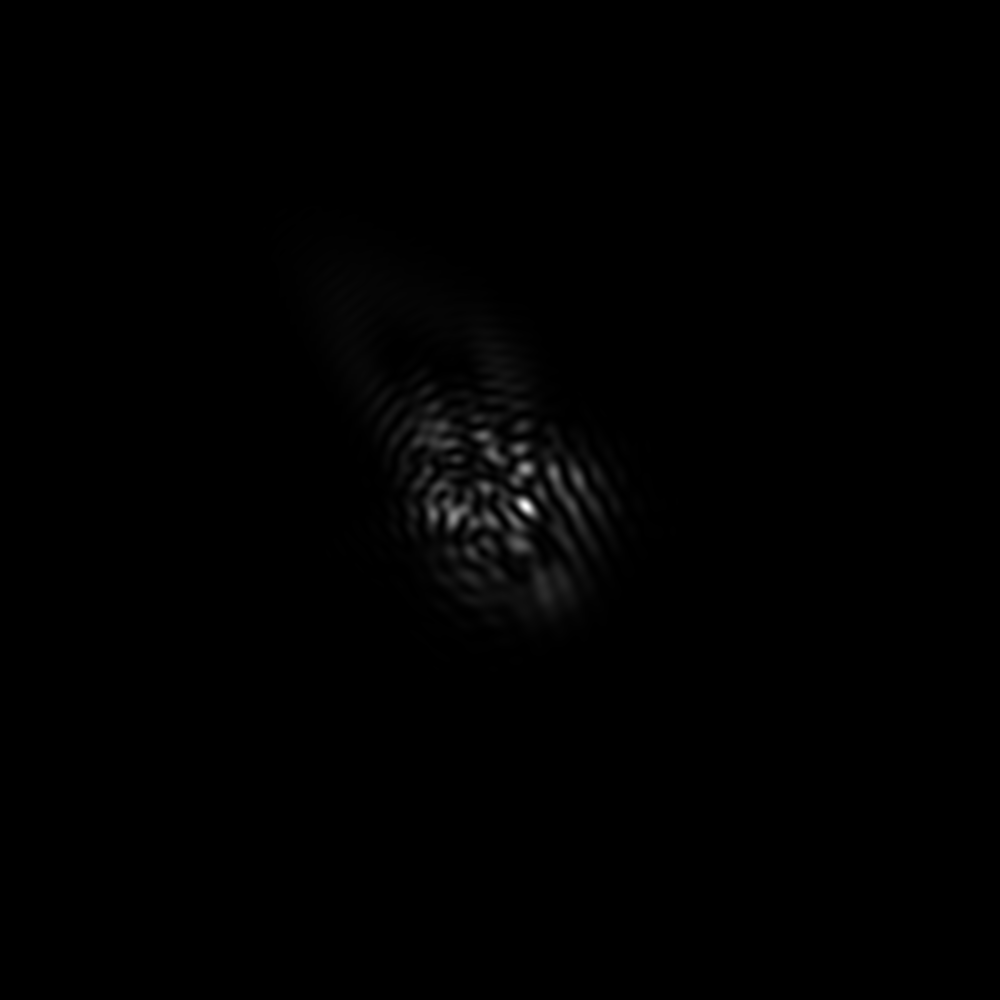
\includegraphics[width=.8\linewidth]{Baldwin_PSF.png}
  \caption{Point Spread Function}
  \label{fig:baldwinpsf}
\end{subfigure}
\caption{HO Wave Aberration and PSF for Baldwin}
\label{fig:baldwin}
\end{figure}

\clearpage

\begin{figure}[H]
\begin{subfigure}{.5\textwidth}
  \centering
  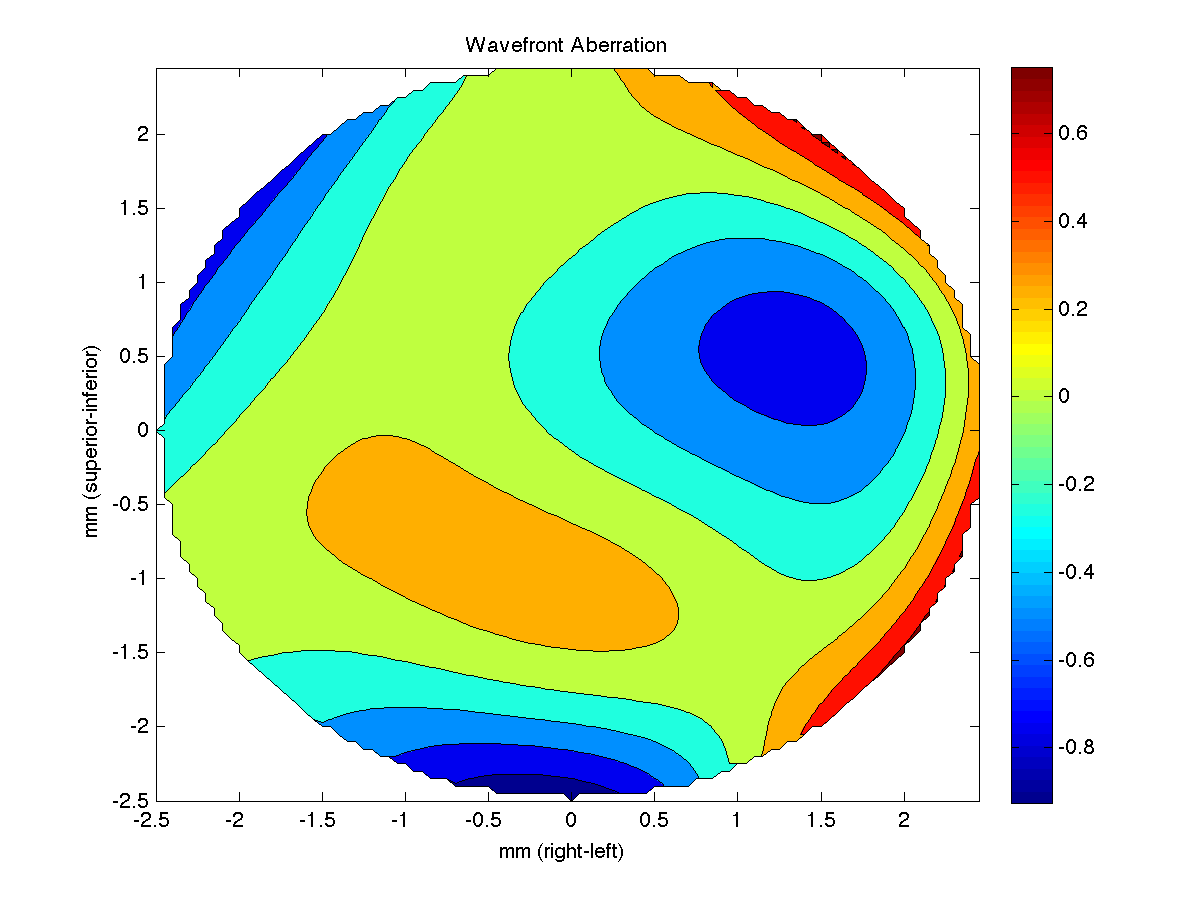
\includegraphics[width=1\linewidth]{Bensaid_WFA.png}
  \caption{High Order Wavefront Aberration}
  \label{fig:bensaidhowa}
\end{subfigure}%
\begin{subfigure}{.5\textwidth}
  \centering
  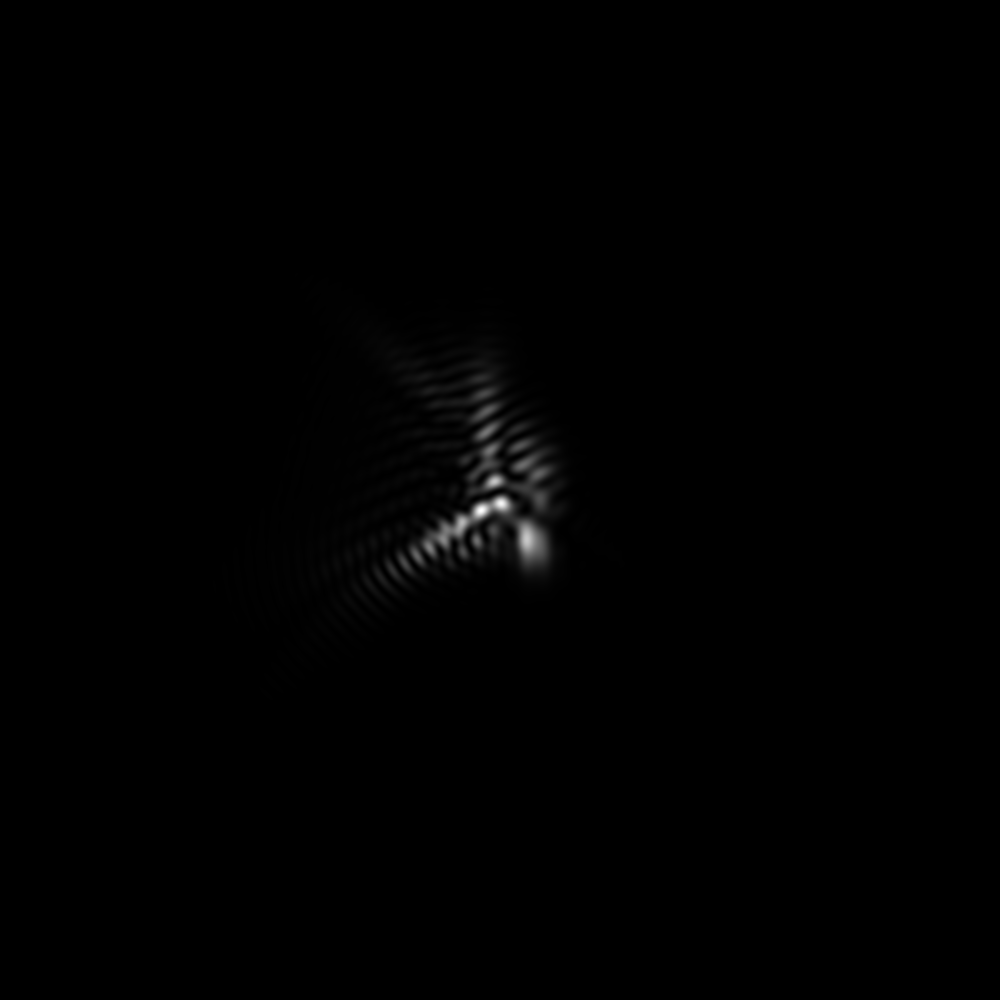
\includegraphics[width=.8\linewidth]{Bensaid_PSF.png}
  \caption{Point Spread Function}
  \label{fig:bensaidpsf}
\end{subfigure}
\caption{HO Wave Aberration and PSF for Bensaid}
\label{fig:bensaid}
\end{figure}


\begin{figure}[H]
\begin{subfigure}{.5\textwidth}
  \centering
  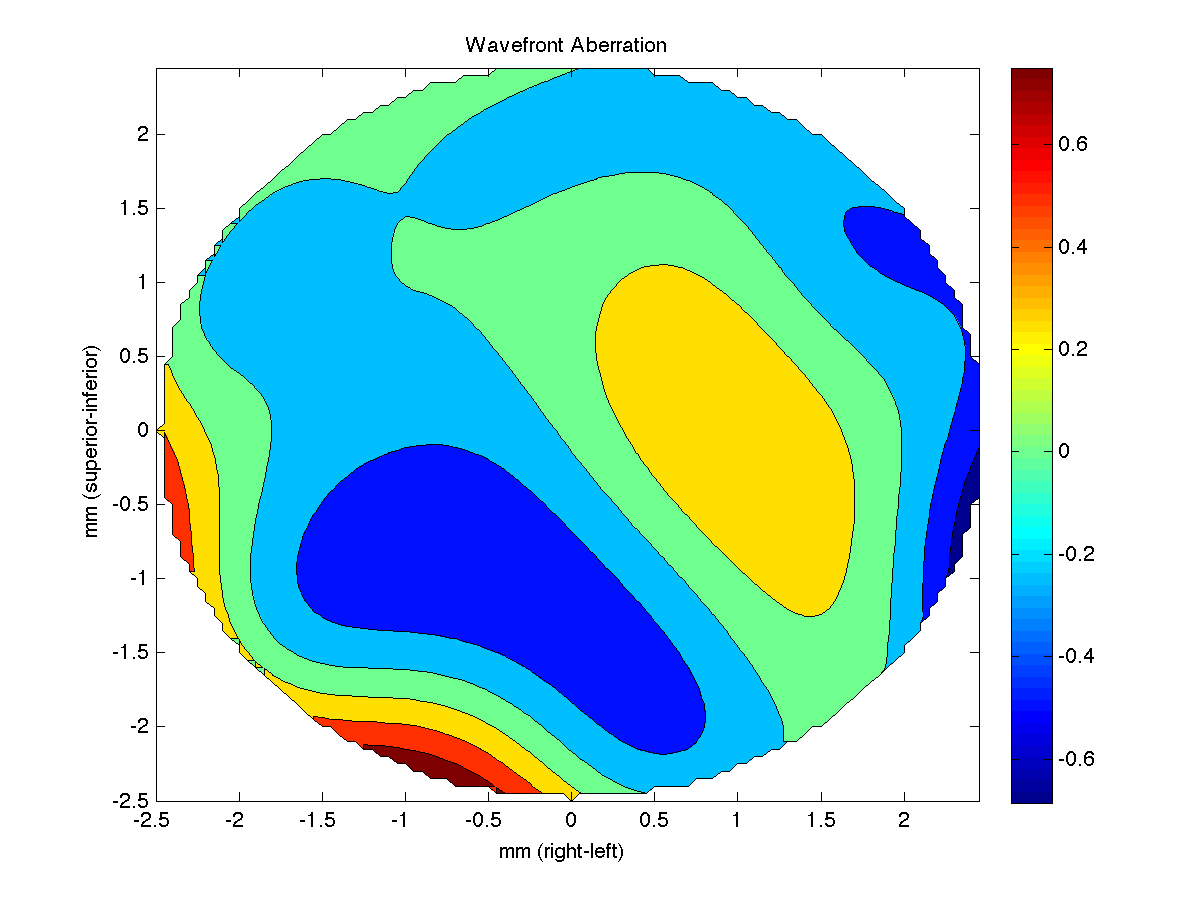
\includegraphics[width=1\linewidth]{Billie_WFA.png}
  \caption{High Order Wavefront Aberration}
  \label{fig:billiehowa}
\end{subfigure}%
\begin{subfigure}{.5\textwidth}
  \centering
  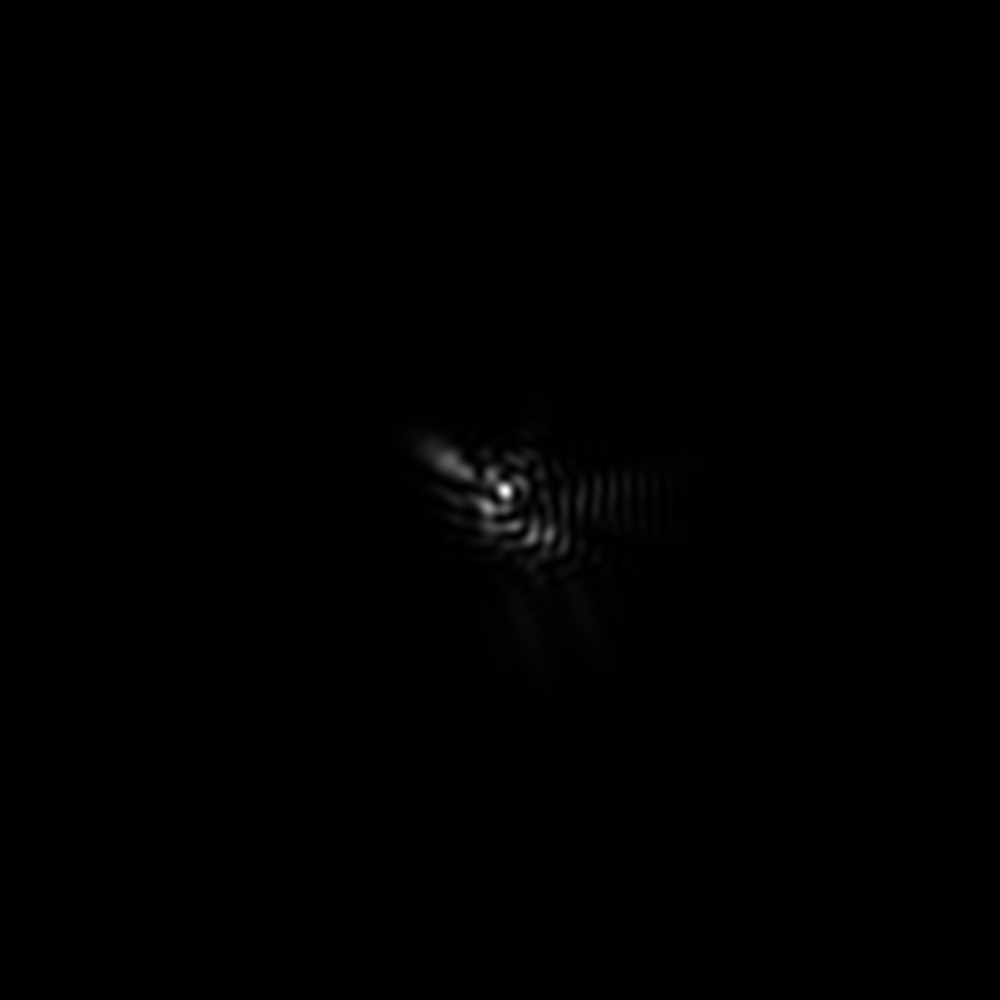
\includegraphics[width=.8\linewidth]{Billie_PSF.png}
  \caption{Point Spread Function}
  \label{fig:billiepsf}
\end{subfigure}
\caption{HO Wave Aberration and PSF for Billie}
\label{fig:billie}
\end{figure}


\clearpage

\begin{figure}[H]
\begin{subfigure}{.5\textwidth}
  \centering
  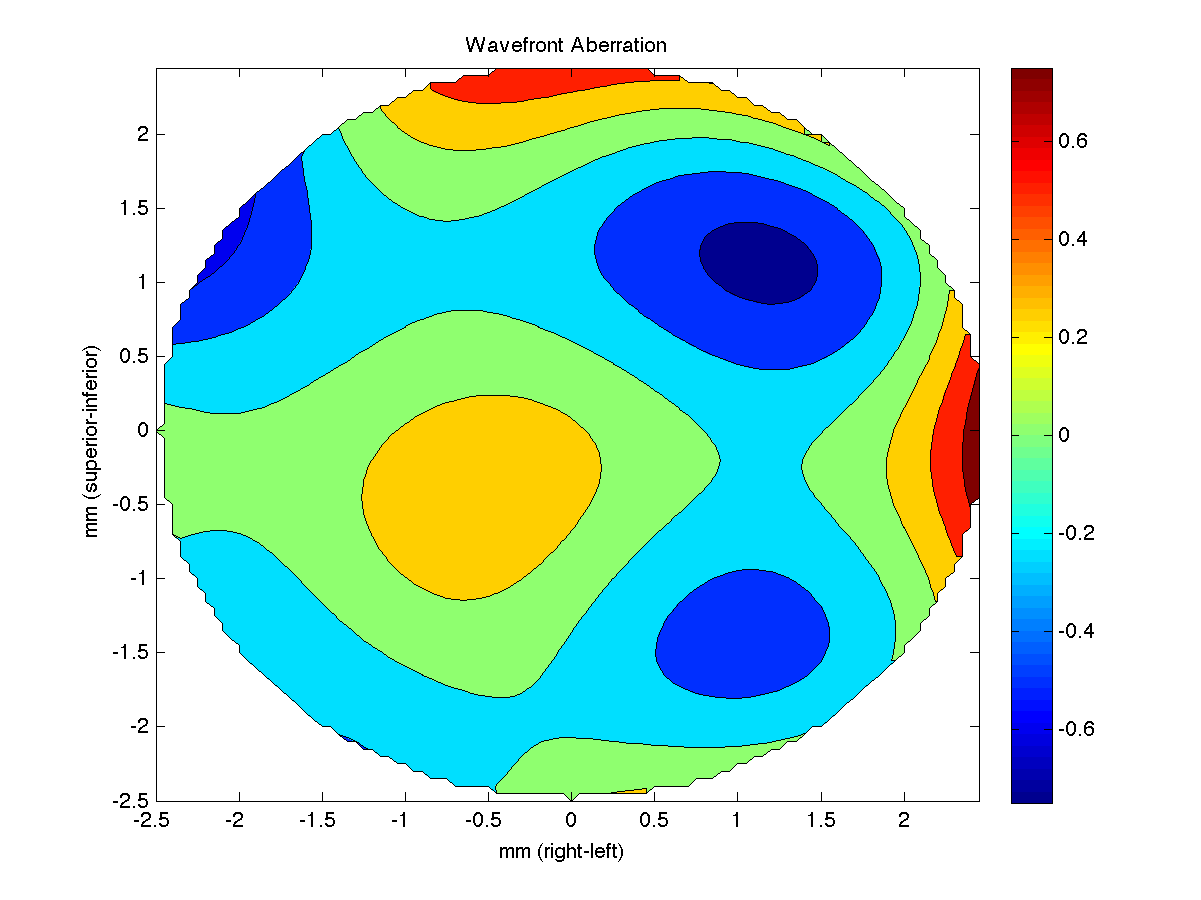
\includegraphics[width=1\linewidth]{Ethan_WFA.png}
  \caption{High Order Wavefront Aberration}
  \label{fig:ethanhowa}
\end{subfigure}%
\begin{subfigure}{.5\textwidth}
  \centering
  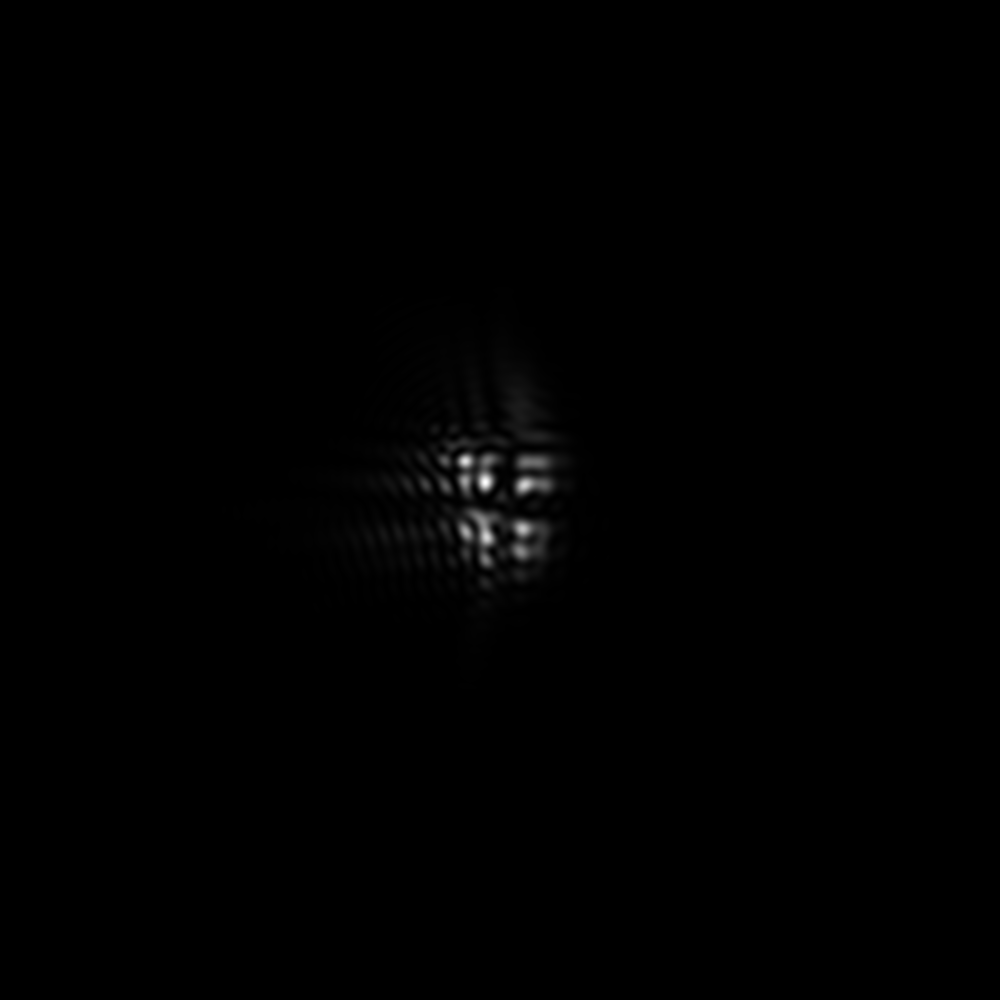
\includegraphics[width=.8\linewidth]{Ethan_PSF.png}
  \caption{Point Spread Function}
  \label{fig:ethanpsf}
\end{subfigure}
\caption{HO Wave Aberration and PSF for Ethan}
\label{fig:ethan}
\end{figure}

\begin{figure}[H]
\begin{subfigure}{.5\textwidth}
  \centering
  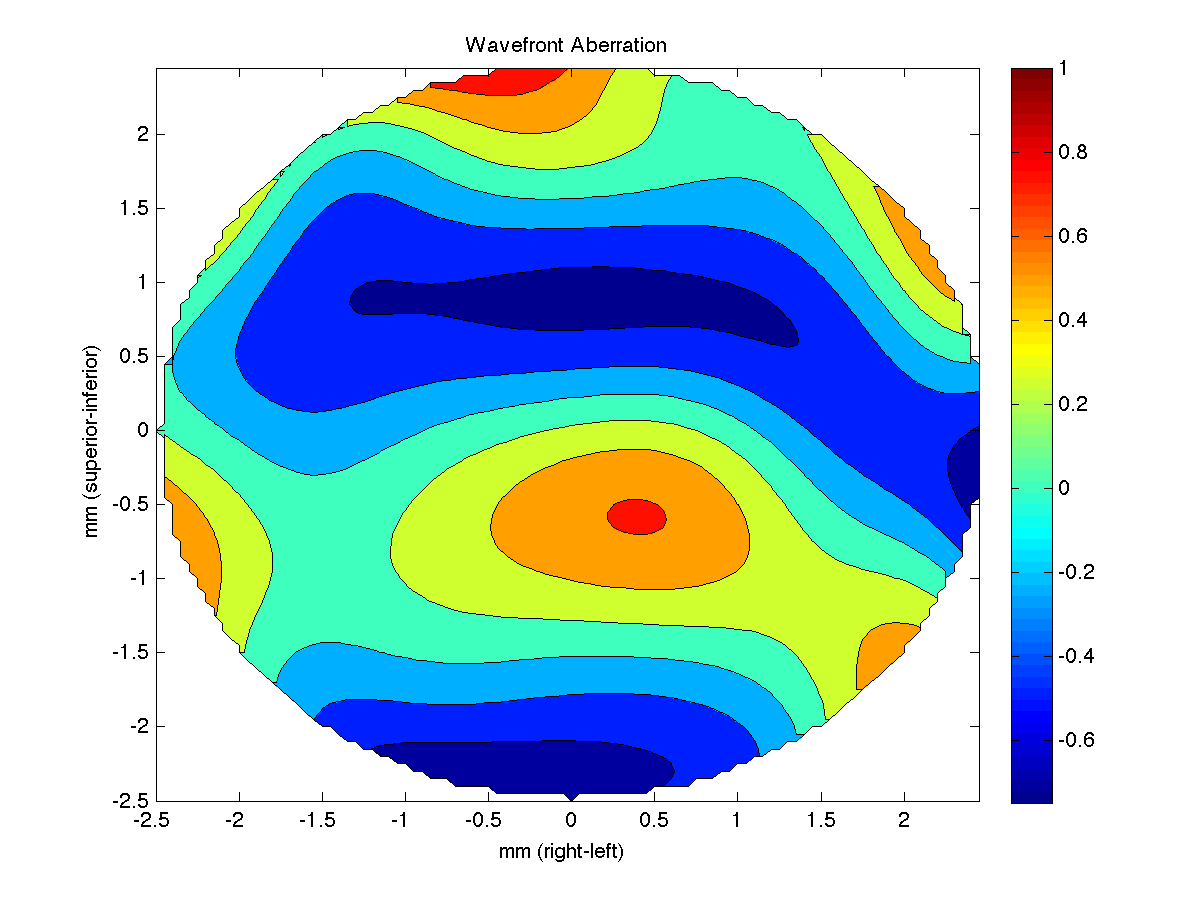
\includegraphics[width=1\linewidth]{Jazzi_WFA.png}
  \caption{High Order Wavefront Aberration}
  \label{fig:jazzihowa}
\end{subfigure}%
\begin{subfigure}{.5\textwidth}
  \centering
  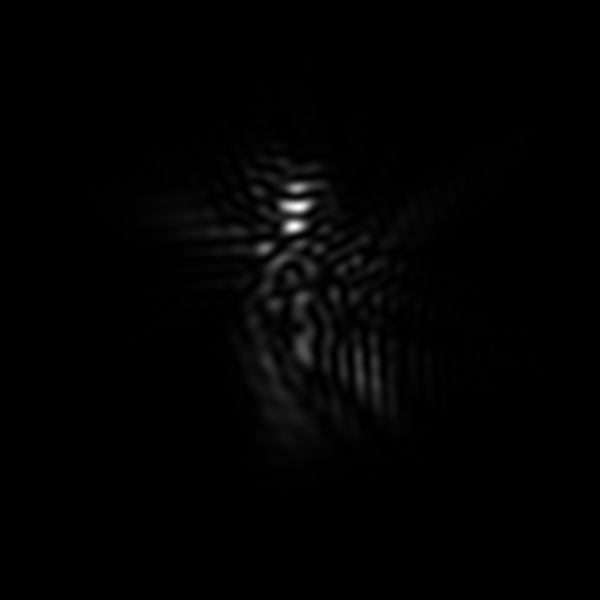
\includegraphics[width=.8\linewidth]{Jazzi_PSF.png}
  \caption{Point Spread Function}
  \label{fig:jazzipsf}
\end{subfigure}
\caption{HO Wave Aberration and PSF for Jazzi}
\label{fig:jazzi}
\end{figure}

\clearpage

\begin{figure}[H]
\begin{subfigure}{.5\textwidth}
  \centering
  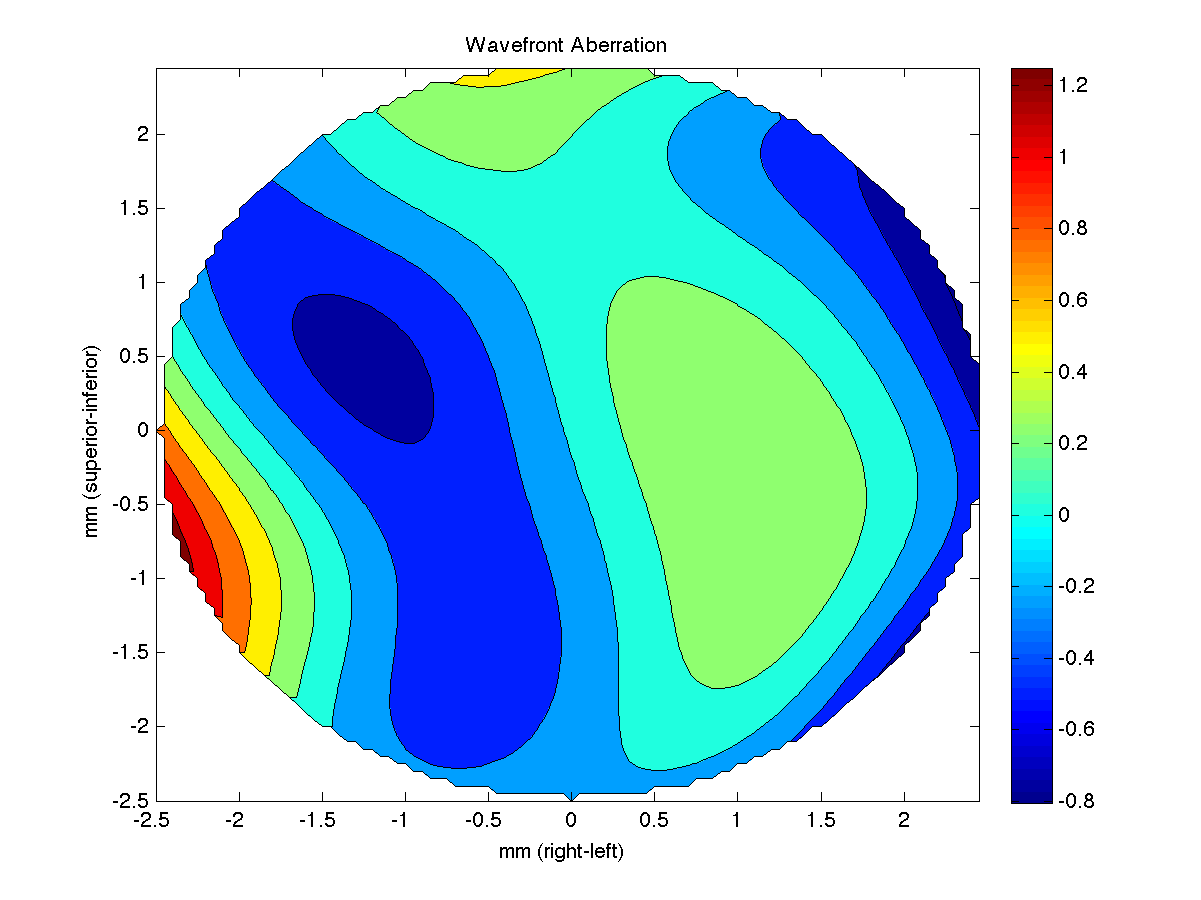
\includegraphics[width=1\linewidth]{Kat_WFA.png}
  \caption{High Order Wavefront Aberration}
  \label{fig:kathowa}
\end{subfigure}%
\begin{subfigure}{.5\textwidth}
  \centering
  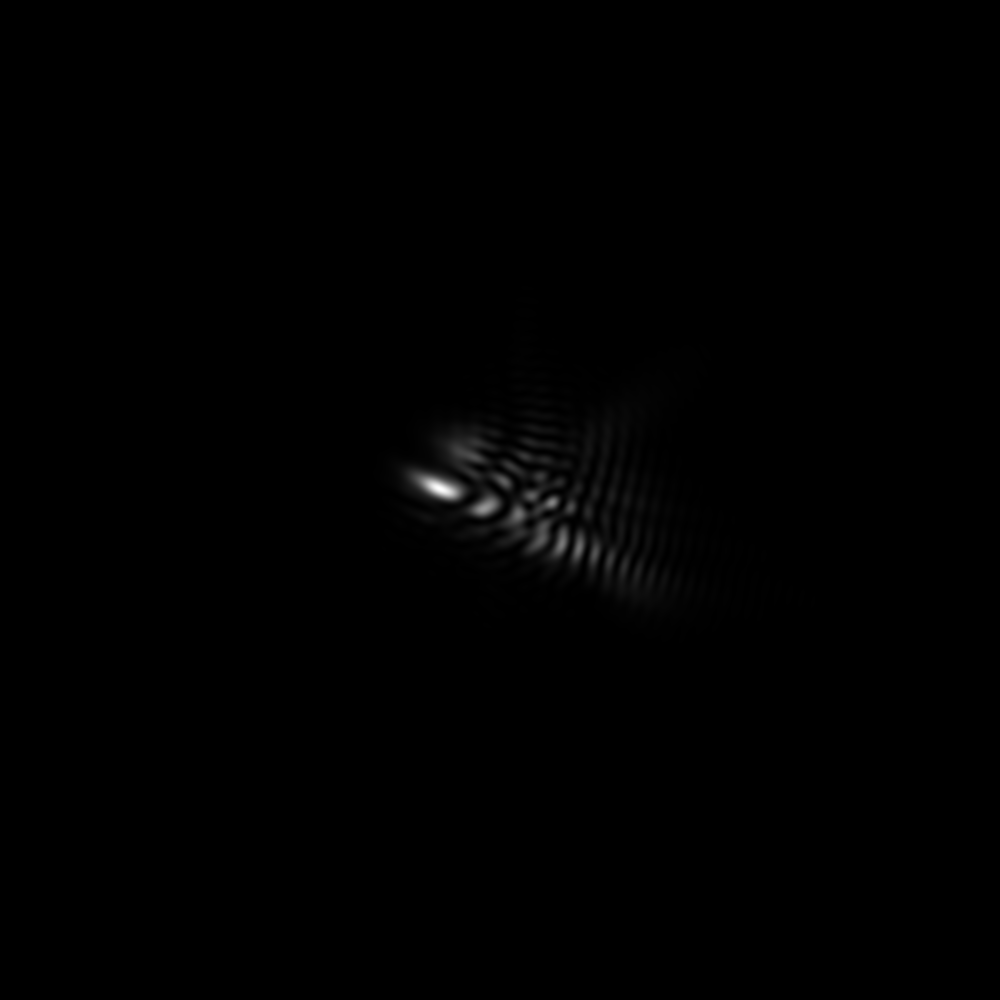
\includegraphics[width=0.8\linewidth]{Kat_PSF.png}
  \caption{Point Spread Function}
  \label{fig:katpsf}
\end{subfigure}
\caption{HO Wave Aberration and PSF for Kat}
\label{fig:kat}
\end{figure}


\begin{figure}[H]
\begin{subfigure}{.5\textwidth}
  \centering
  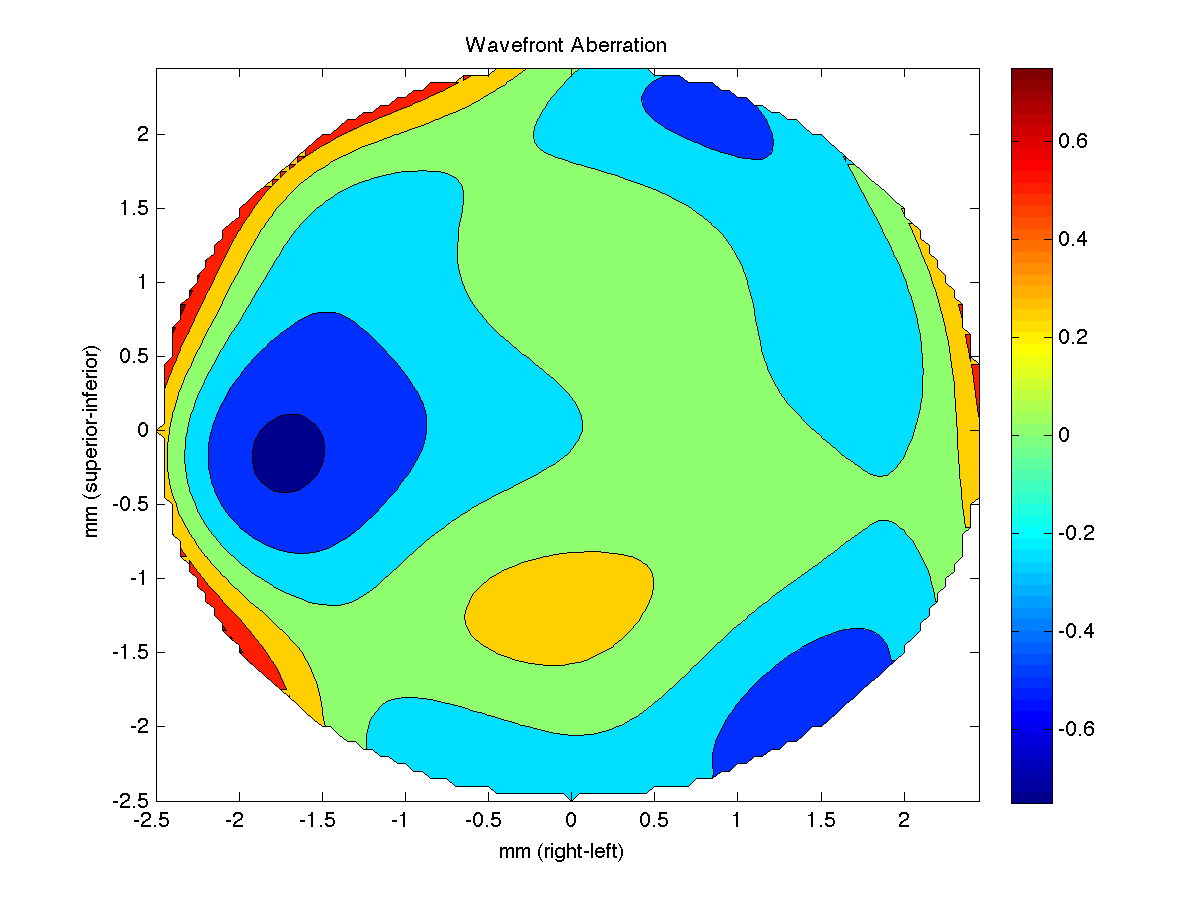
\includegraphics[width=1\linewidth]{Linyue_WFA.png}
  \caption{High Order Wavefront Aberration}
  \label{fig:linyuehowa}
\end{subfigure}%
\begin{subfigure}{.5\textwidth}
  \centering
  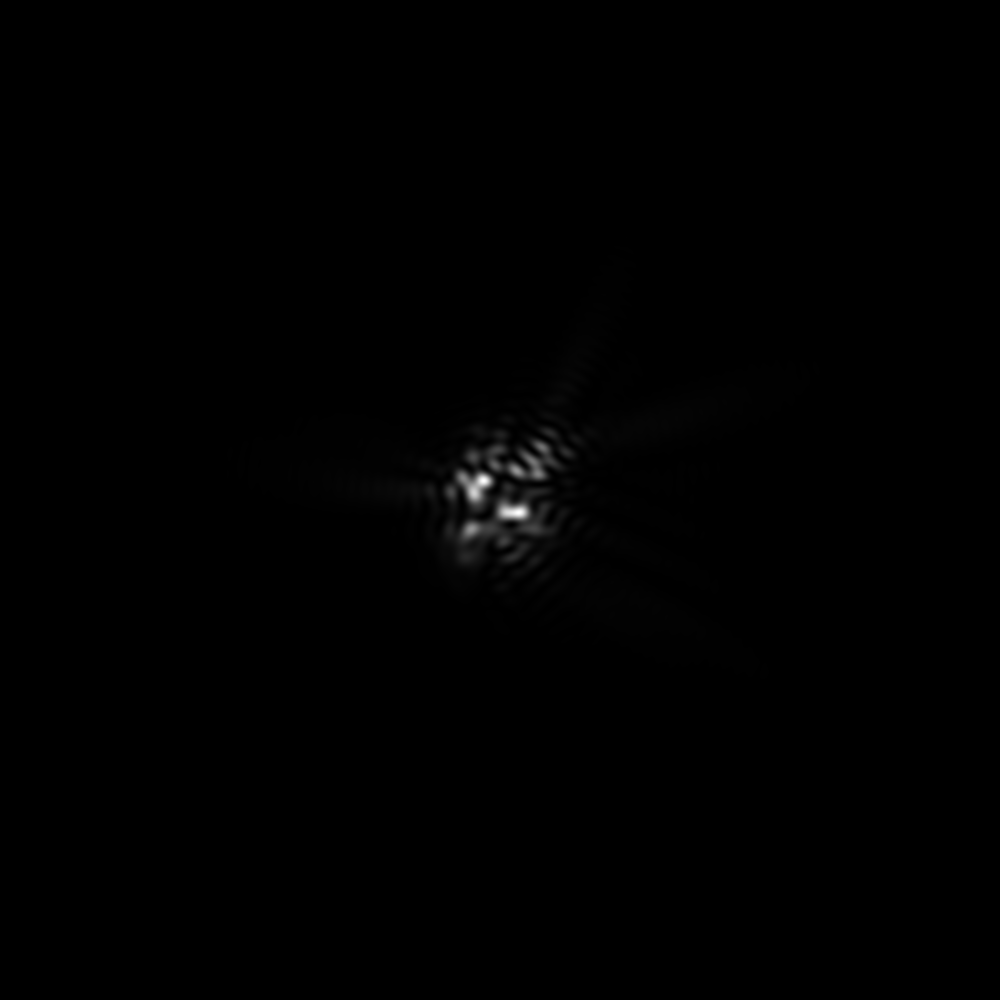
\includegraphics[width=.8\linewidth]{Linyue_PSF.png}
  \caption{Point Spread Function}
  \label{fig:linyuepsf}
\end{subfigure}
\caption{HO Wave Aberration and PSF for Linyue}
\label{fig:linyue}
\end{figure}


\clearpage

\begin{figure}[H]
\begin{subfigure}{.5\textwidth}
  \centering
  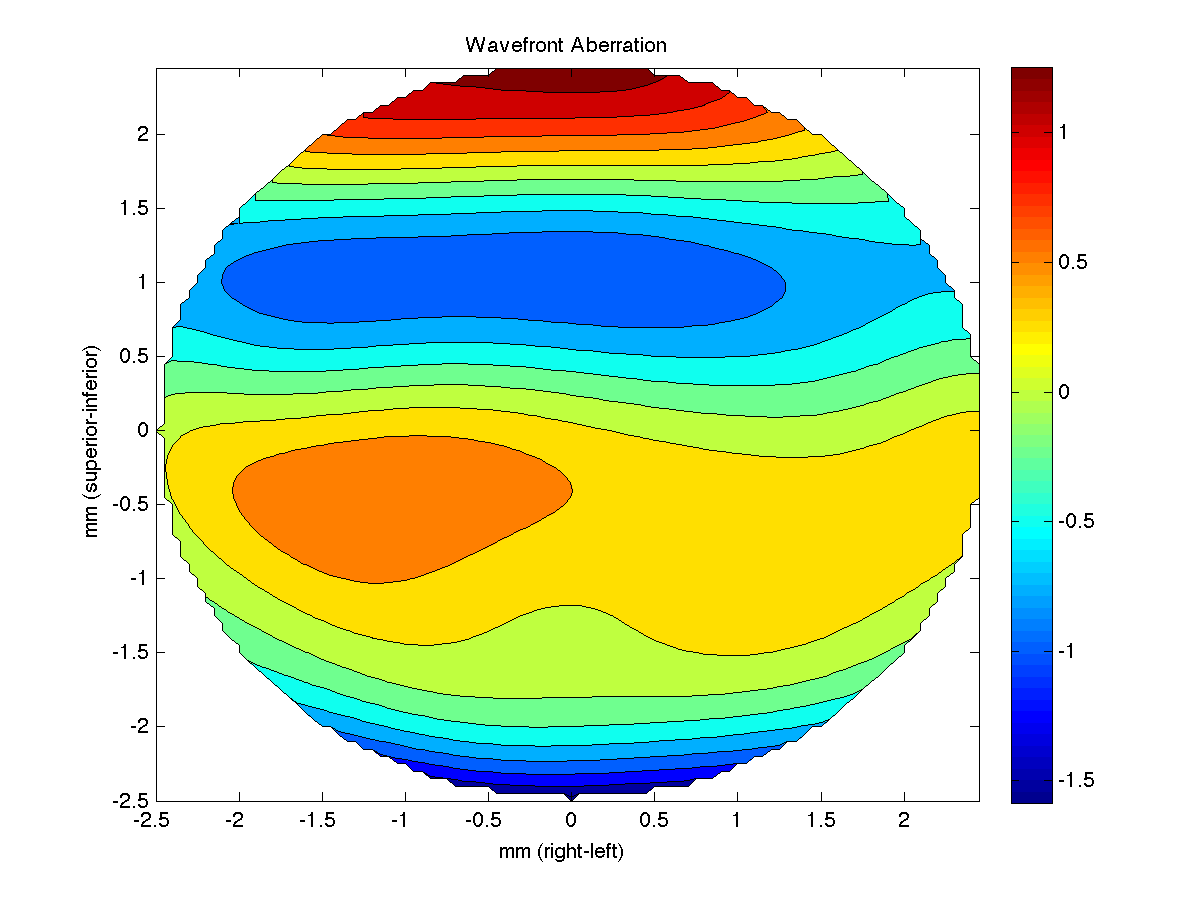
\includegraphics[width=1\linewidth]{Liz_WFA.png}
  \caption{High Order Wavefront Aberration}
  \label{fig:lizhowa}
\end{subfigure}%
\begin{subfigure}{.5\textwidth}
  \centering
  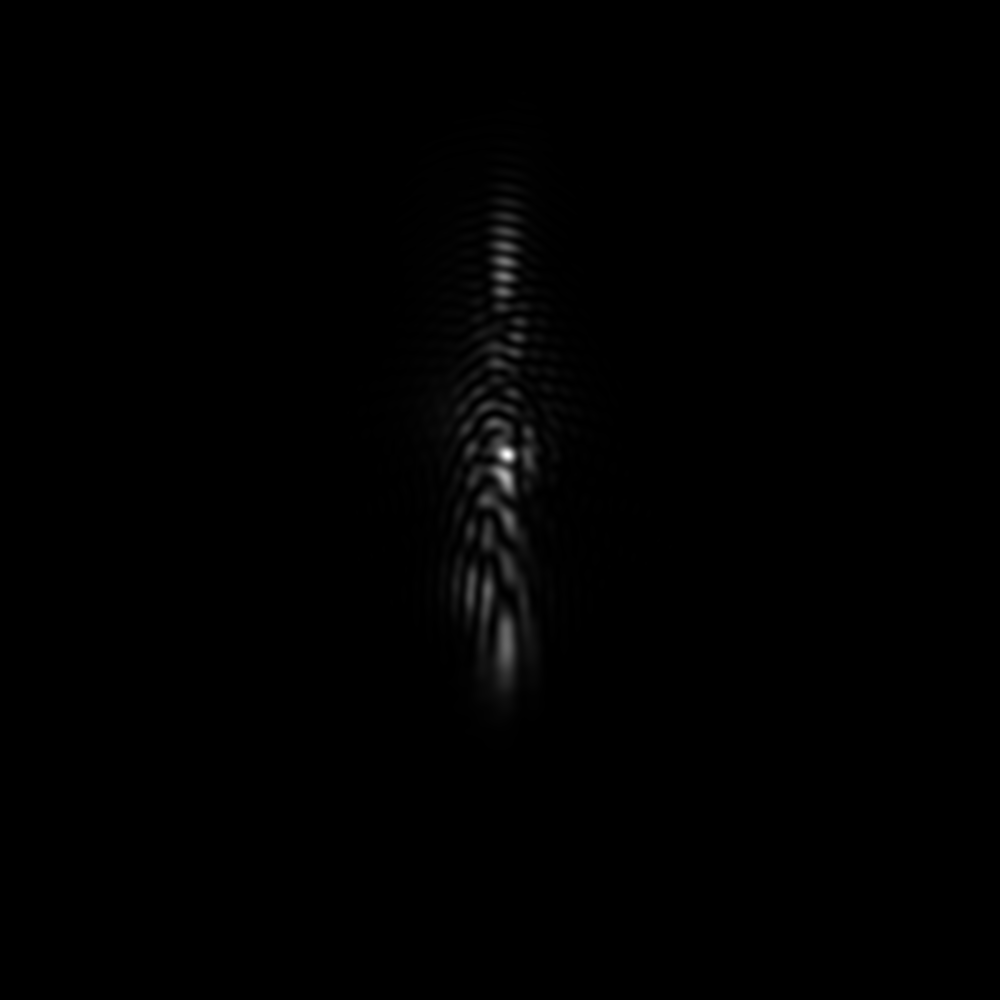
\includegraphics[width=.8\linewidth]{Liz_PSF.png}
  \caption{Point Spread Function}
  \label{fig:lizpsf}
\end{subfigure}
\caption{HO Wave Aberration and PSF for Liz}
\label{fig:liz}
\end{figure}

\begin{figure}[H]
\begin{subfigure}{.5\textwidth}
  \centering
  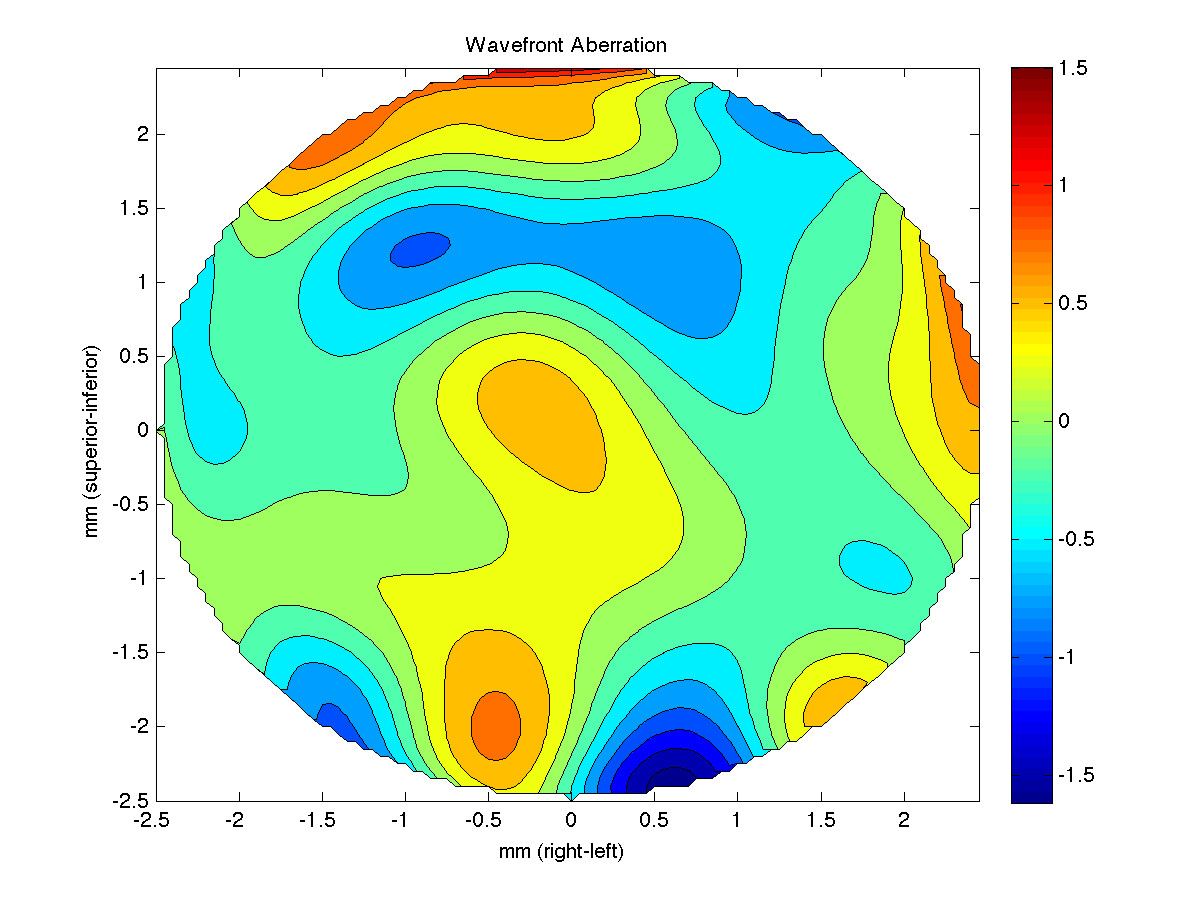
\includegraphics[width=1\linewidth]{Michael_WFA.png}
  \caption{High Order Wavefront Aberration}
  \label{fig:michaelhowa}
\end{subfigure}%
\begin{subfigure}{.5\textwidth}
  \centering
  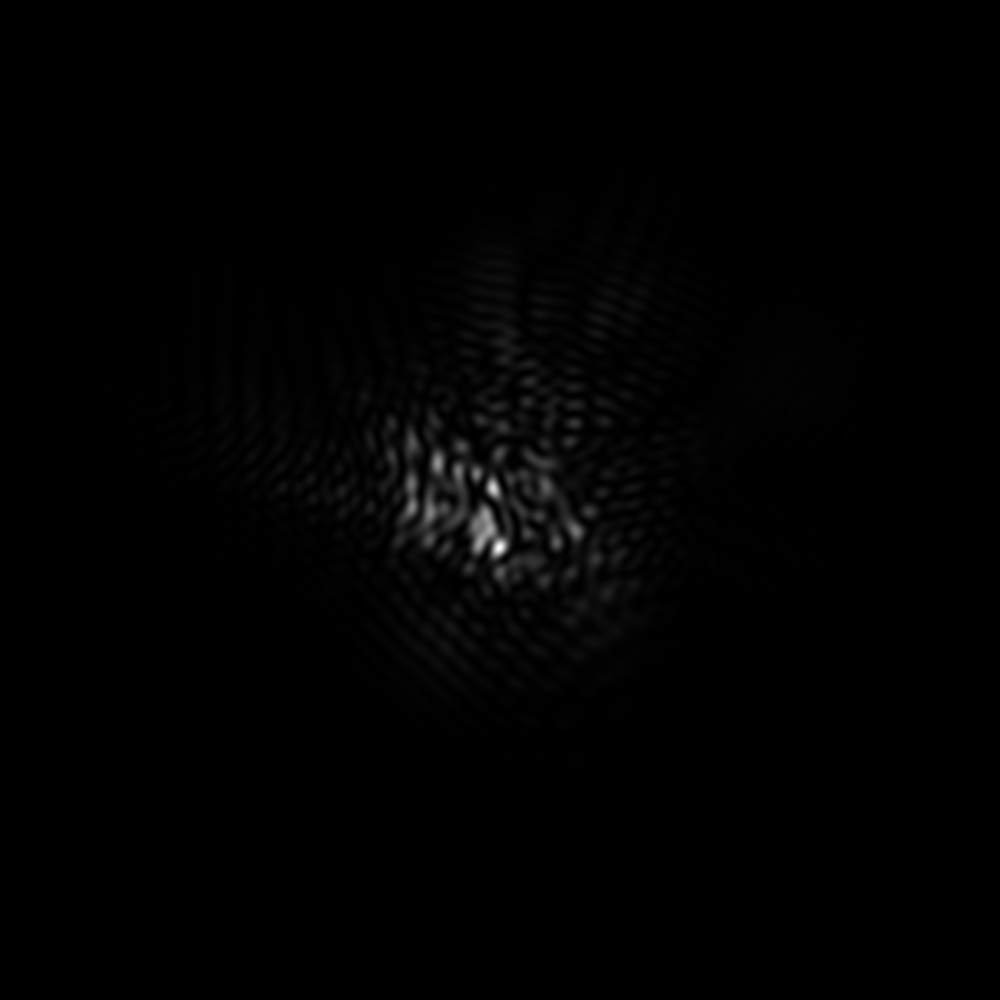
\includegraphics[width=.8\linewidth]{Michael_PSF.png}
  \caption{Point Spread Function}
  \label{fig:michaelpsf}
\end{subfigure}
\caption{HO Wave Aberration and PSF for Michael}
\label{fig:michael}
\end{figure}

\clearpage

\begin{figure}[H]
\begin{subfigure}{.5\textwidth}
  \centering
  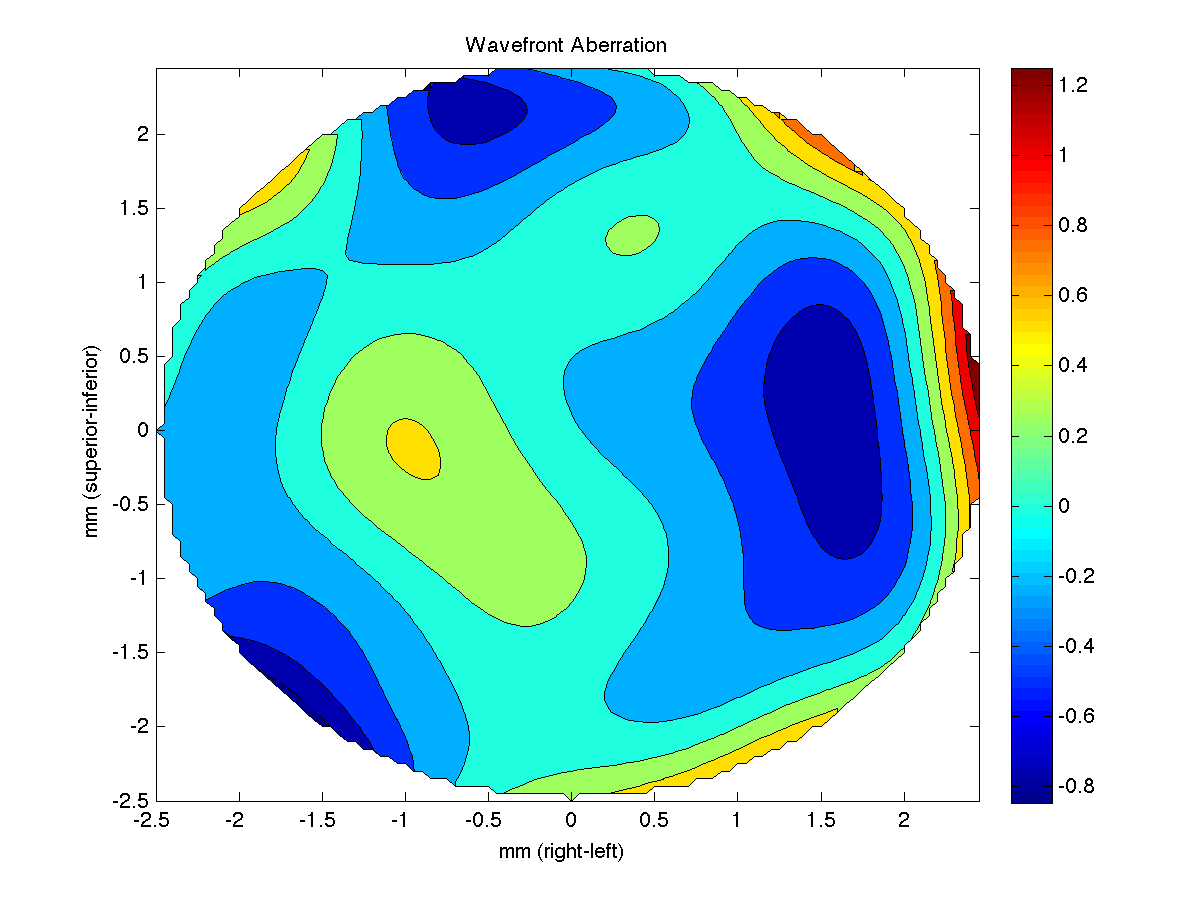
\includegraphics[width=1\linewidth]{Natalie_WFA.png}
  \caption{High Order Wavefront Aberration}
  \label{fig:nataliehowa}
\end{subfigure}%
\begin{subfigure}{.5\textwidth}
  \centering
  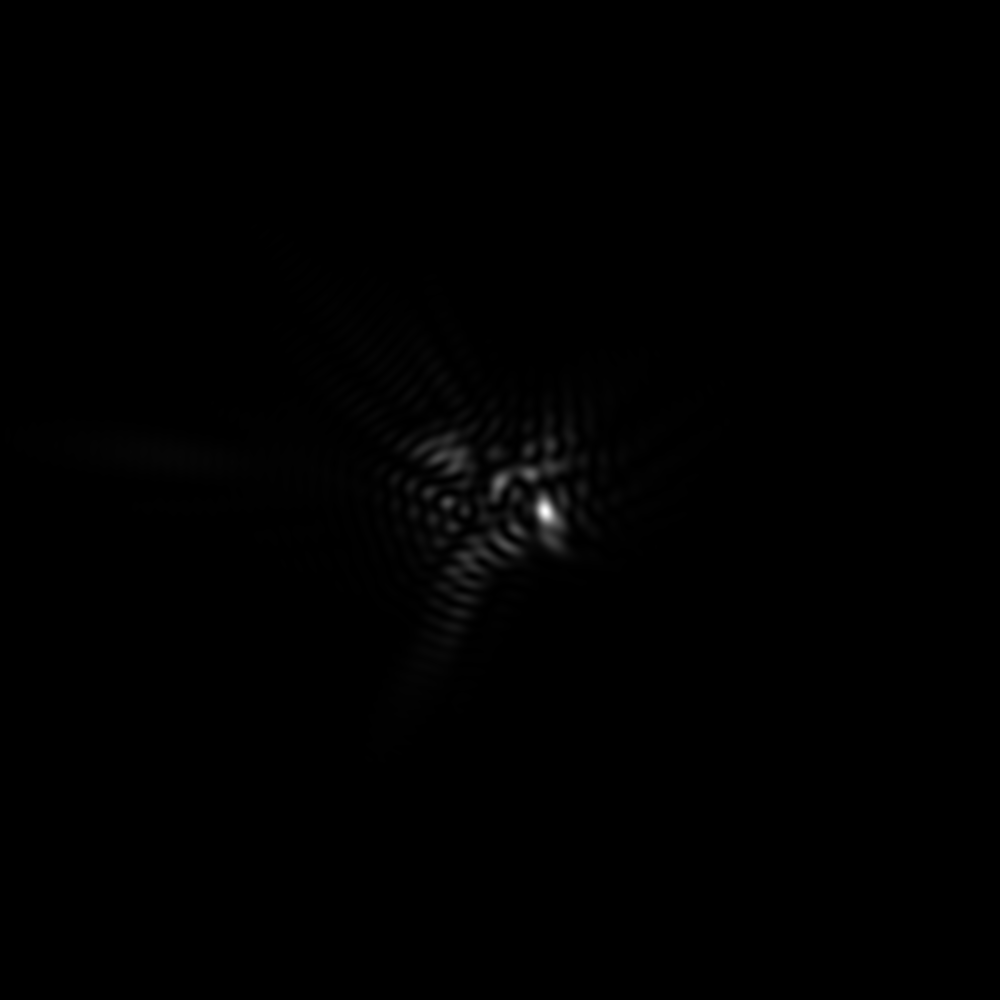
\includegraphics[width=.8\linewidth]{Natalie_PSF.png}
  \caption{Point Spread Function}
  \label{fig:nataliepsf}
\end{subfigure}
\caption{HO Wave Aberration and PSF for Natalie}
\label{fig:natalie}
\end{figure}


\begin{figure}[H]
\begin{subfigure}{.5\textwidth}
  \centering
  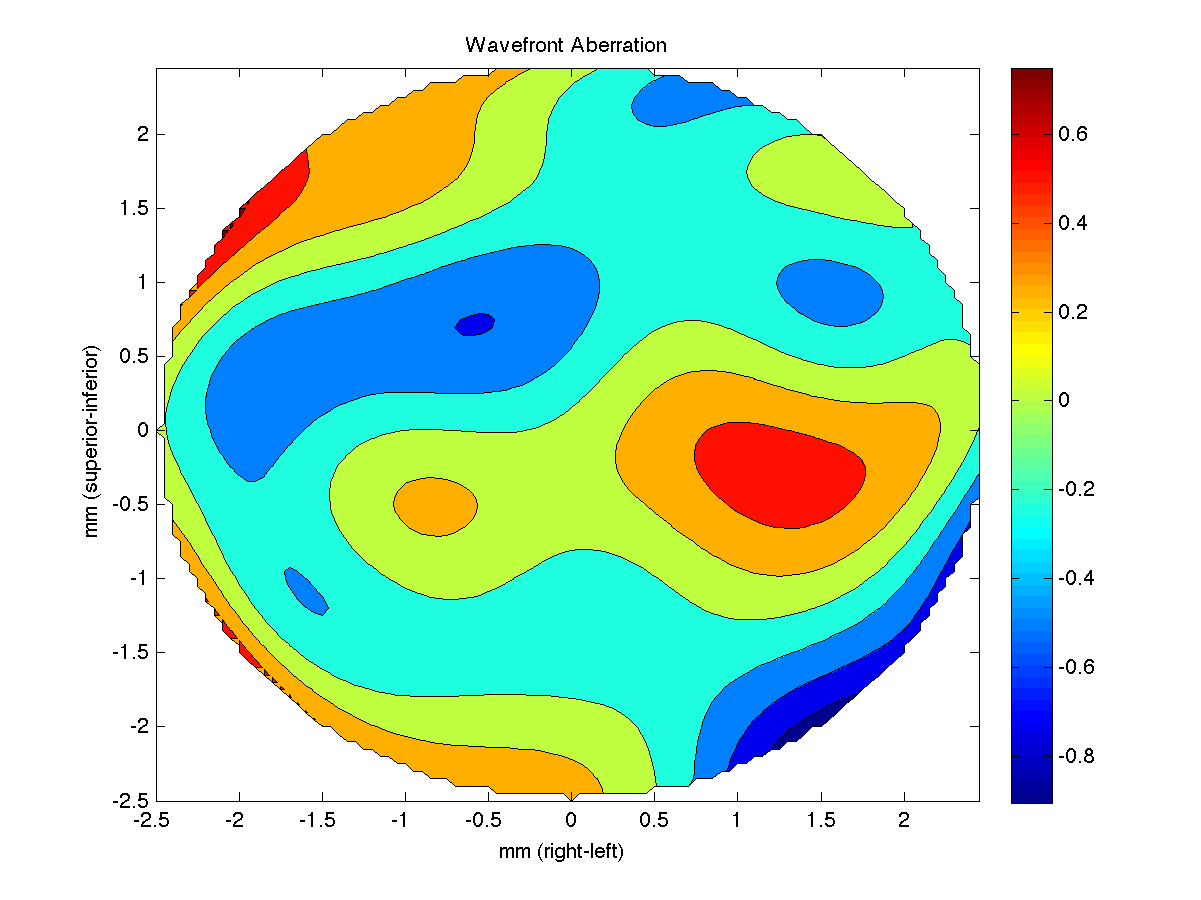
\includegraphics[width=1\linewidth]{Peter_WFA.png}
  \caption{High Order Wavefront Aberration}
  \label{fig:peterhowa}
\end{subfigure}%
\begin{subfigure}{.5\textwidth}
  \centering
  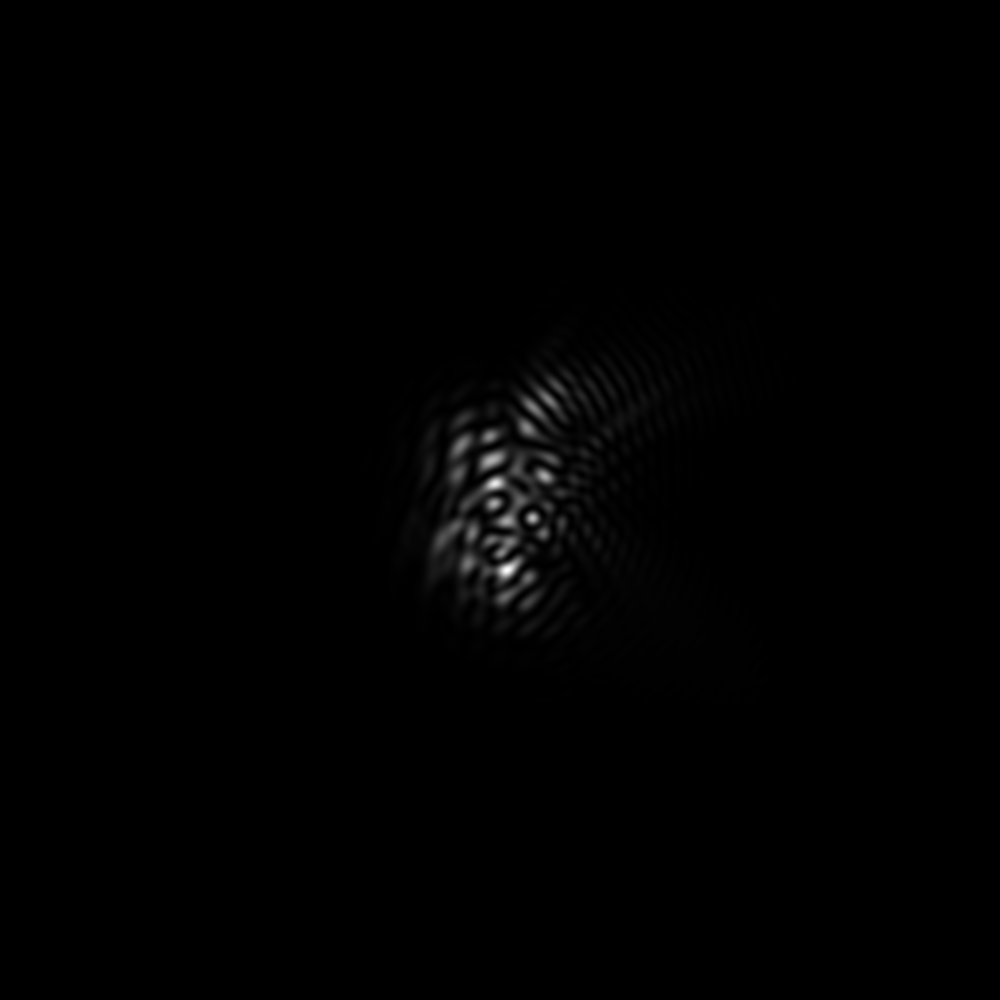
\includegraphics[width=.8\linewidth]{Peter_PSF.png}
  \caption{Point Spread Function}
  \label{fig:peterpsf}
\end{subfigure}
\caption{HO Wave Aberration and PSF for Peter}
\label{fig:peter}
\end{figure}

\clearpage

\begin{figure}[H]
\begin{subfigure}{.5\textwidth}
  \centering
  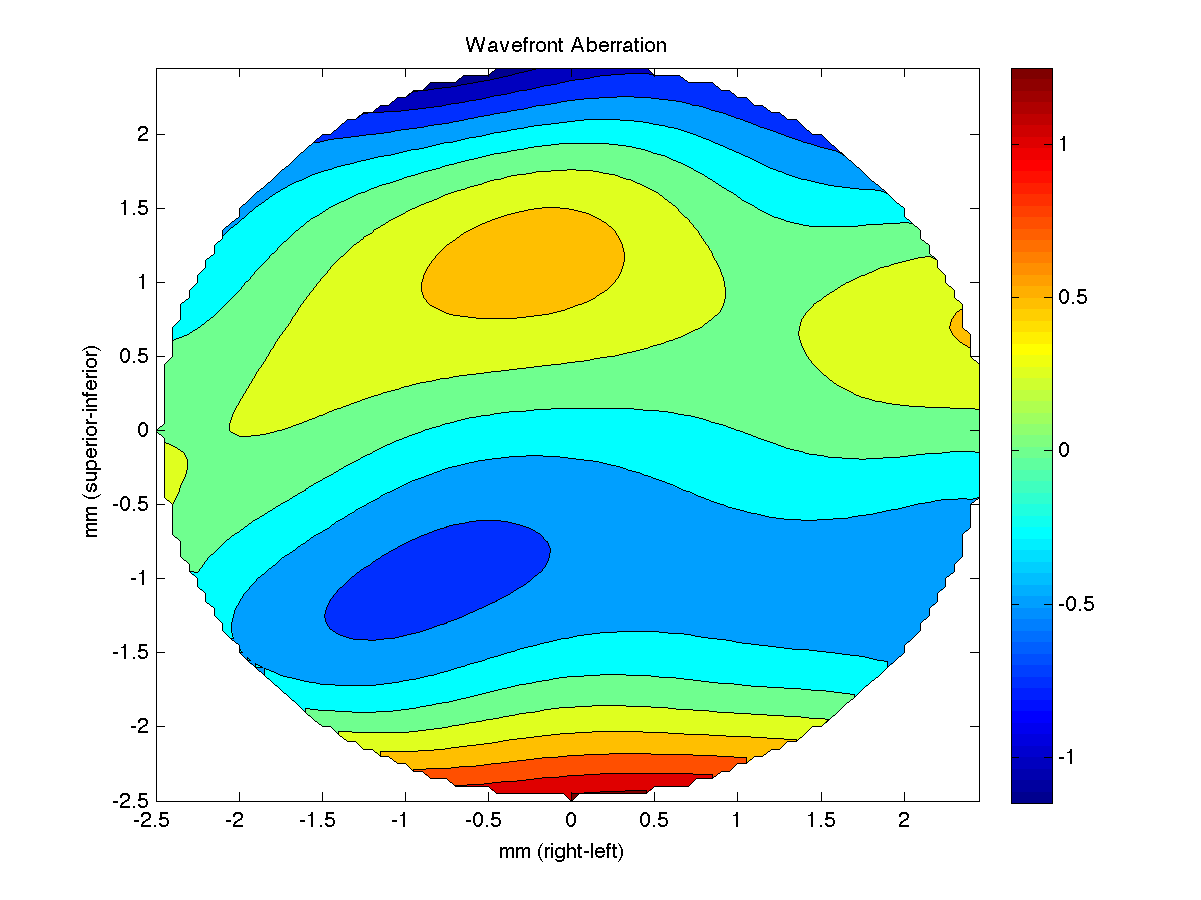
\includegraphics[width=1\linewidth]{Sanam_WFA.png}
  \caption{High Order Wavefront Aberration}
  \label{fig:sanamhowa}
\end{subfigure}%
\begin{subfigure}{.5\textwidth}
  \centering
  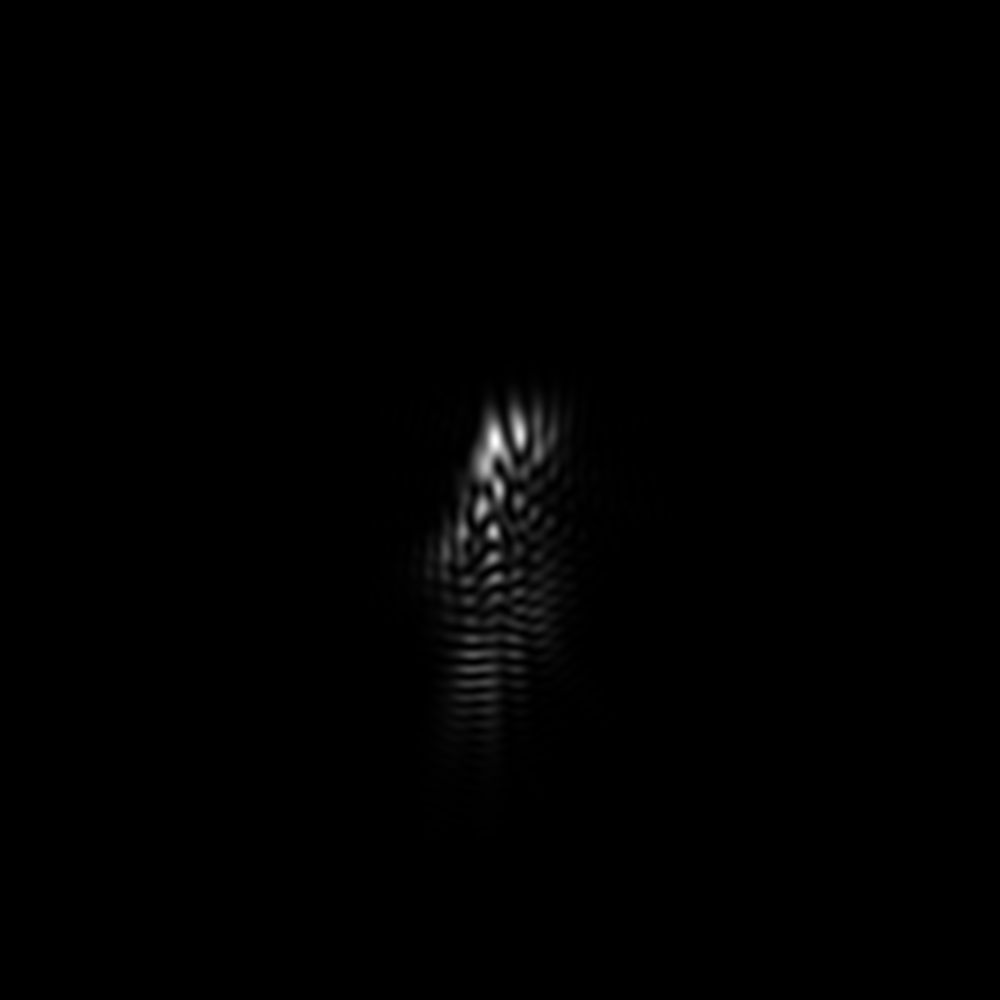
\includegraphics[width=.8\linewidth]{Sanam_PSF.png}
  \caption{Point Spread Function}
  \label{fig:sanampsf}
\end{subfigure}
\caption{HO Wave Aberration and PSF for Sanam}
\label{fig:sanam}
\end{figure}

\begin{figure}[H]
\begin{subfigure}{.5\textwidth}
  \centering
  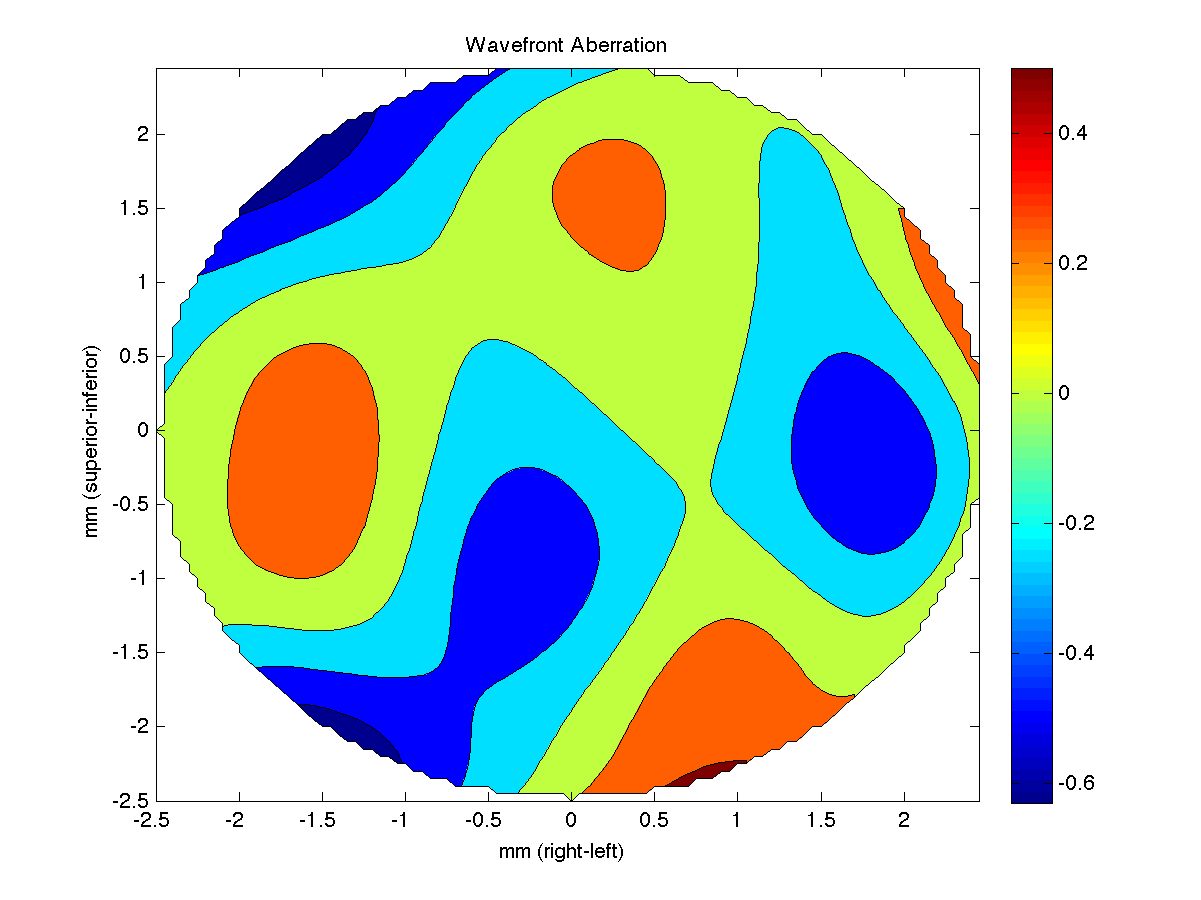
\includegraphics[width=1\linewidth]{Sarah_WFA.png}
  \caption{High Order Wavefront Aberration}
  \label{fig:sarahhowa}
\end{subfigure}%
\begin{subfigure}{.5\textwidth}
  \centering
  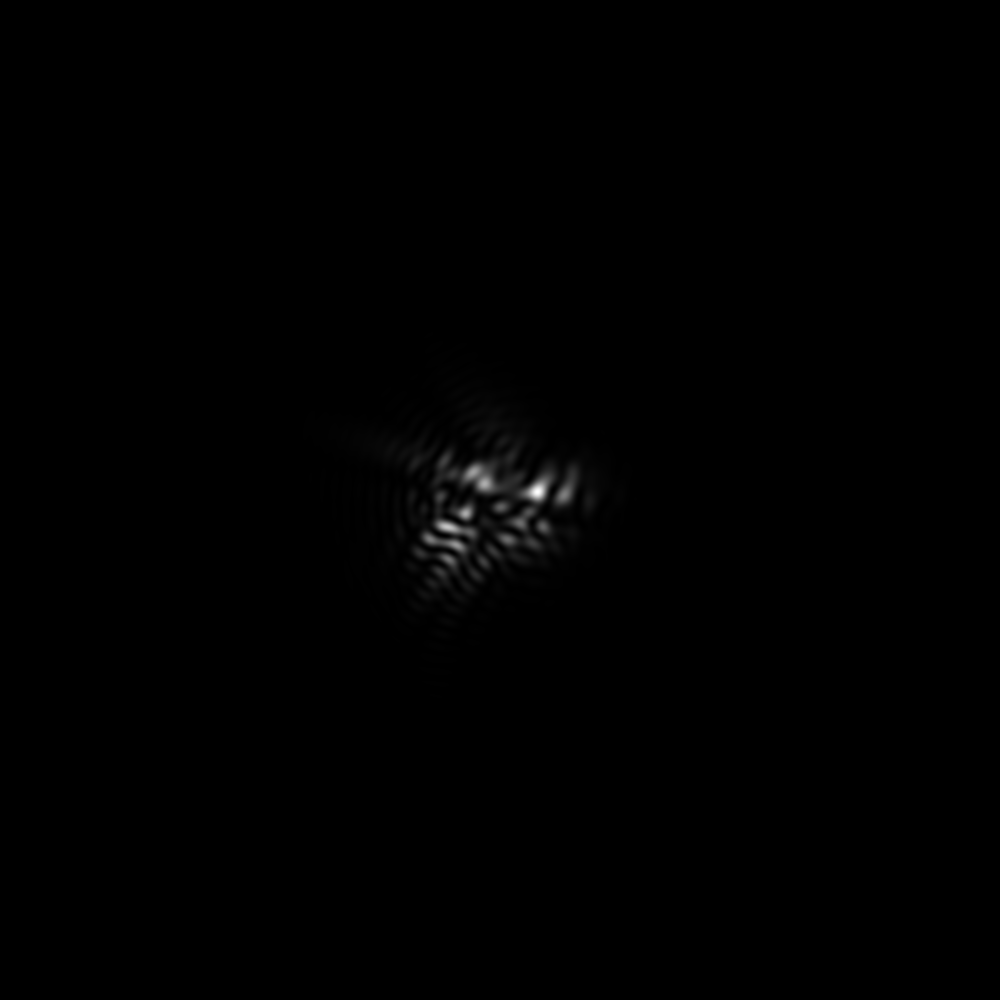
\includegraphics[width=.8\linewidth]{Sarah_PSF.png}
  \caption{Point Spread Function}
  \label{fig:sarahpsf}
\end{subfigure}
\caption{HO Wave Aberration and PSF for Sarah}
\label{fig:sarah}
\end{figure}


\clearpage


\begin{figure}[H]
\begin{subfigure}{.5\textwidth}
  \centering
  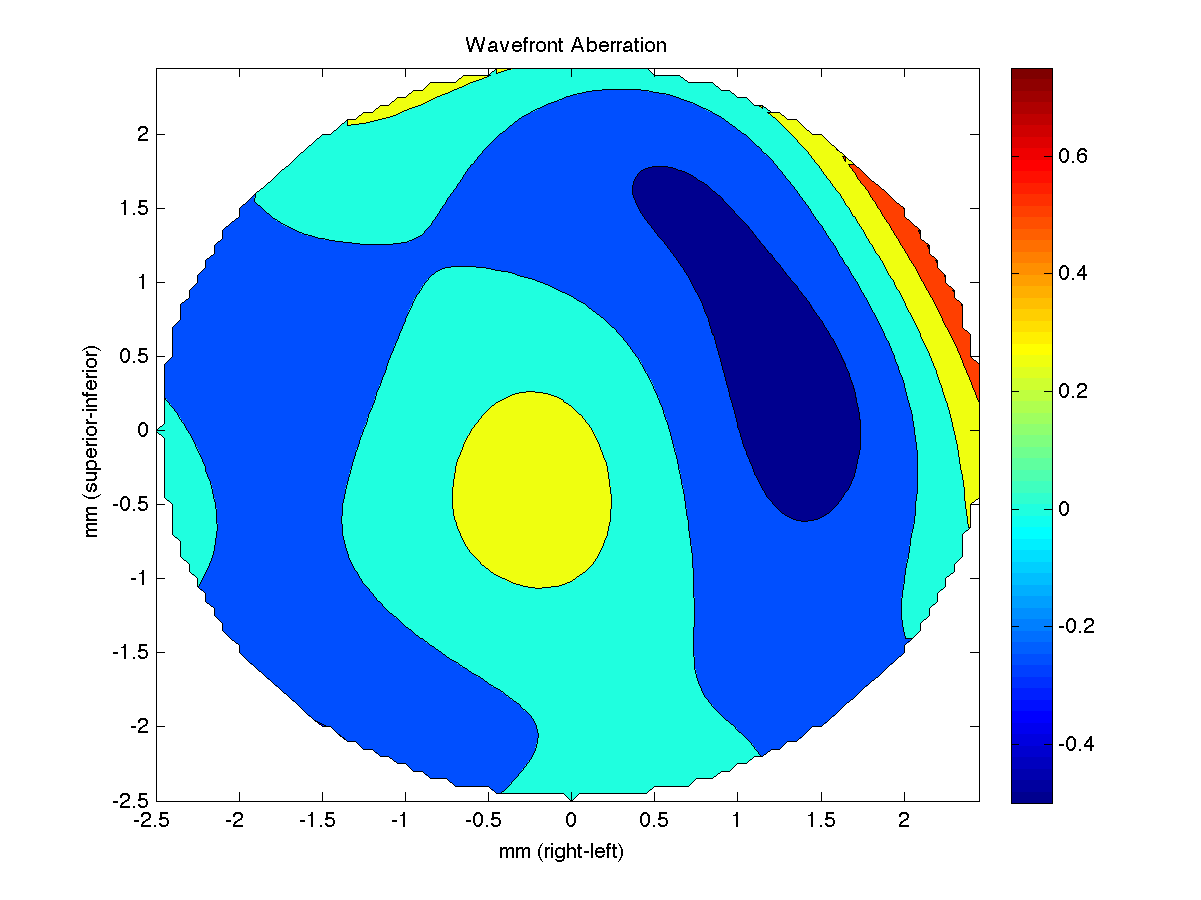
\includegraphics[width=1\linewidth]{Sylvain_WFA.png}
  \caption{High Order Wavefront Aberration}
  \label{fig:sylvainhowa}
\end{subfigure}%
\begin{subfigure}{.5\textwidth}
  \centering
  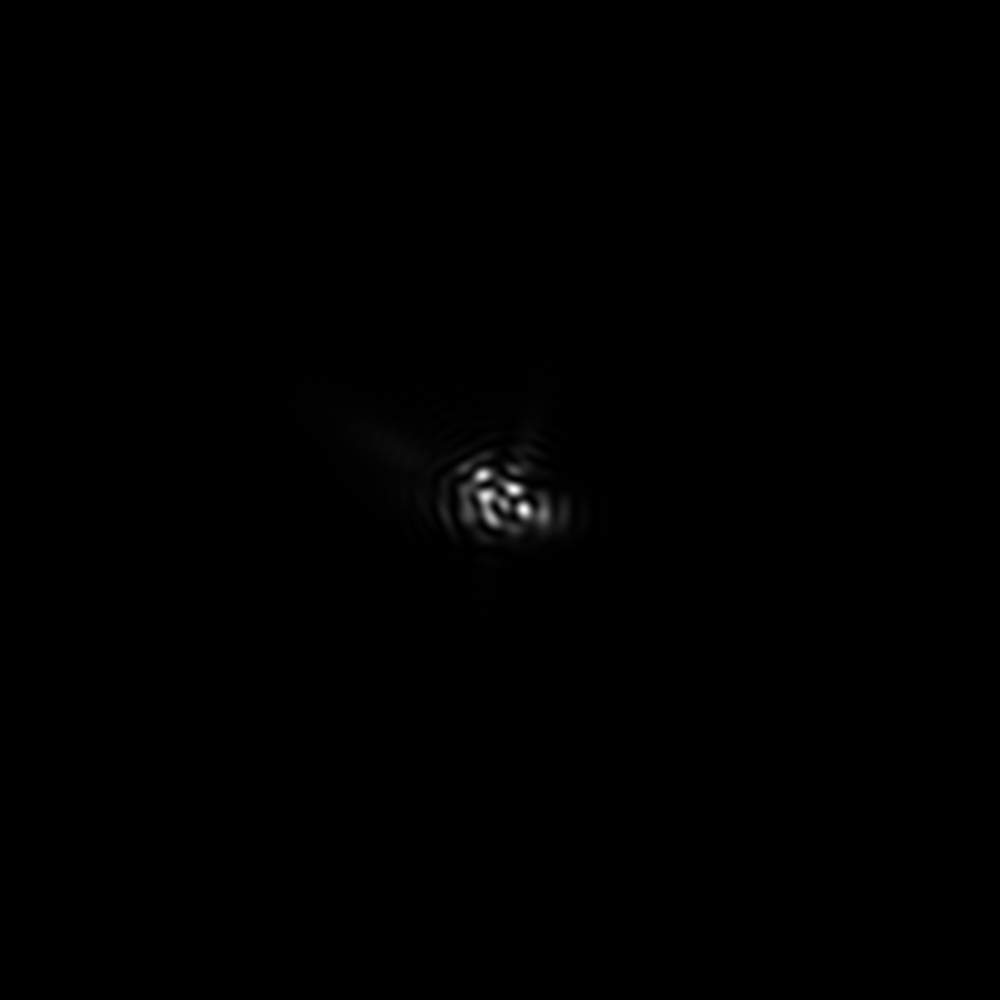
\includegraphics[width=.8\linewidth]{Sylvain_PSF.png}
  \caption{Point Spread Function}
  \label{fig:sylvainpsf}
\end{subfigure}
\caption{HO Wave Aberration and PSF for Sylvain}
\label{fig:sylvain}
\end{figure}

\begin{figure}[H]
\begin{subfigure}{.5\textwidth}
  \centering
  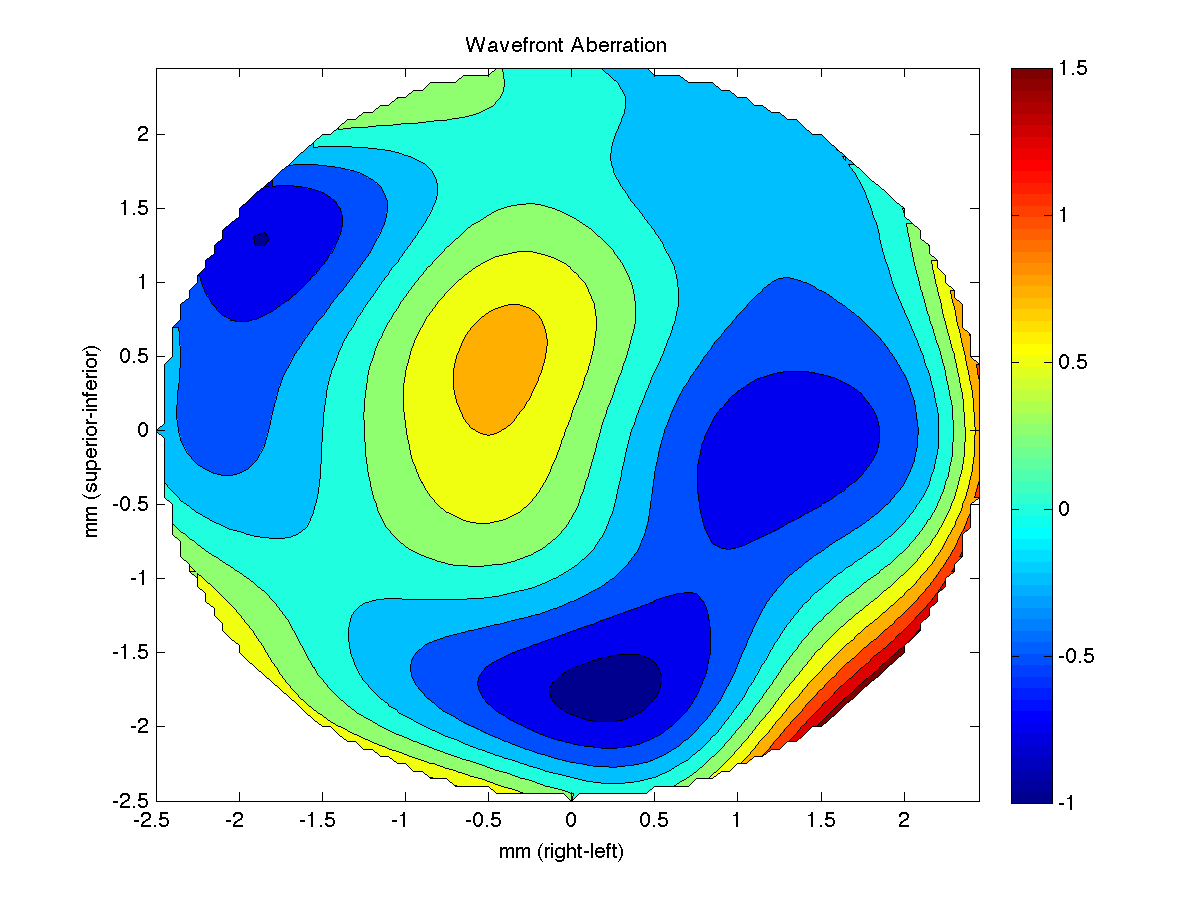
\includegraphics[width=1\linewidth]{Vasha_WFA.png}
  \caption{High Order Wavefront Aberration}
  \label{fig:vashahowa}
\end{subfigure}%
\begin{subfigure}{.5\textwidth}
  \centering
  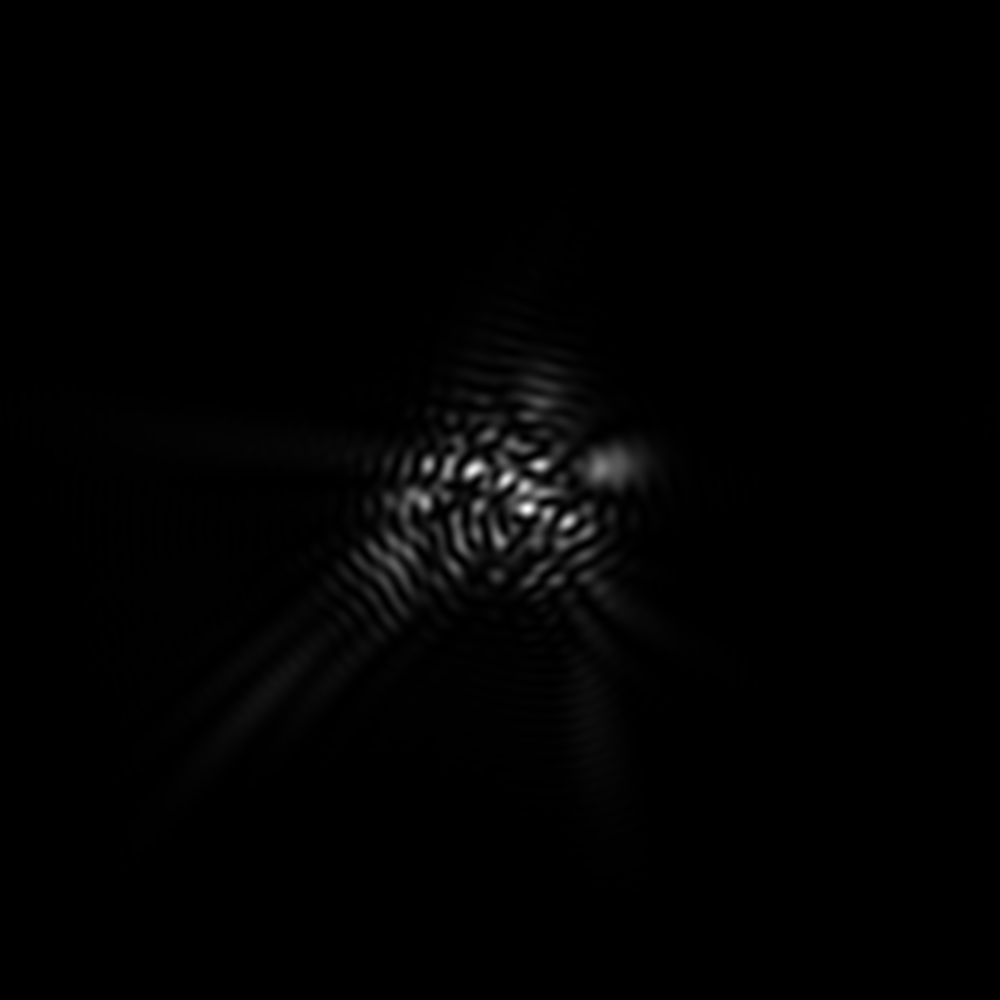
\includegraphics[width=.8\linewidth]{Vasha_PSF.png}
  \caption{Point Spread Function}
  \label{fig:vashapsf}
\end{subfigure}
\caption{HO Wave Aberration and PSF for Vasha}
\label{fig:vasha}
\end{figure}

\clearpage

\subsubsection{High Order Radial Average MTFs}
Here we plot the Modulation Transfer Functions for each student. The Modulation Transfer Functions describe the amount of contrast that can pass through the aberration taking into account the increasing spatial frequency (closeness of lines) of an image.

\begin{figure}[h]
  \centering
    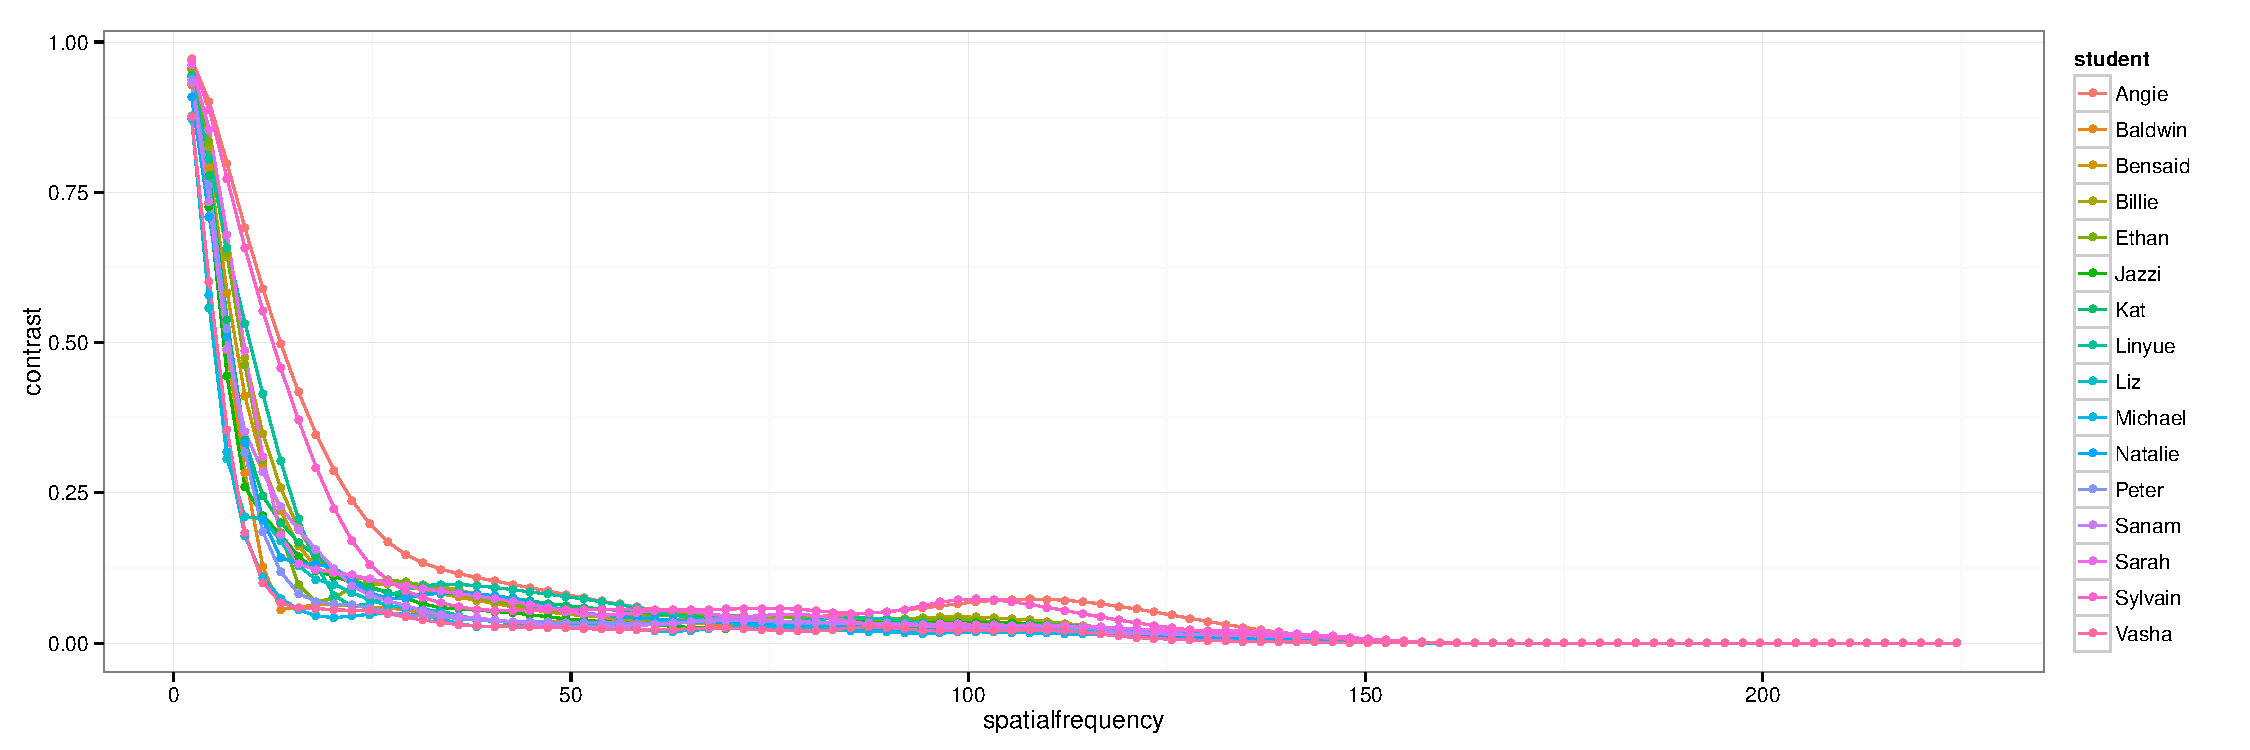
\includegraphics[width=1\linewidth]{mtfs.pdf}
  \caption{radial average MTF plot for all students}
  \label{fig:mtfs}
\end{figure}

All of our eyes perform well at low spatial frequency, but the two eyes that perform distinctly better than all others even at relatively high frequencies are Angie and Sylvain.

\subsection{Three Sets of Zernike coefficients}
Now we pick three students, and do further in-depth analysis on their ZPs, specifically looking at how their values effect RMS, Strehl, and MTF as a result of different defocus levels. We look at defocus ranging from -1 to +1 Diopters, in step sizes of 0.25D. Note that astygmatism terms $Z_-2^2$ and $Z_2^2$ are set to zero before calculation. I will choose myself, an example of strong aberration, Angie, and example of low aberration, and Liz, because she has an interesting looking PSF.

\subsubsection{RMS \& Strehl as a fucntion of defocus}
RMS \& Strehl values for our 3 students plotted as a function of defocus. \

\begin{figure}[H]
  \centering
    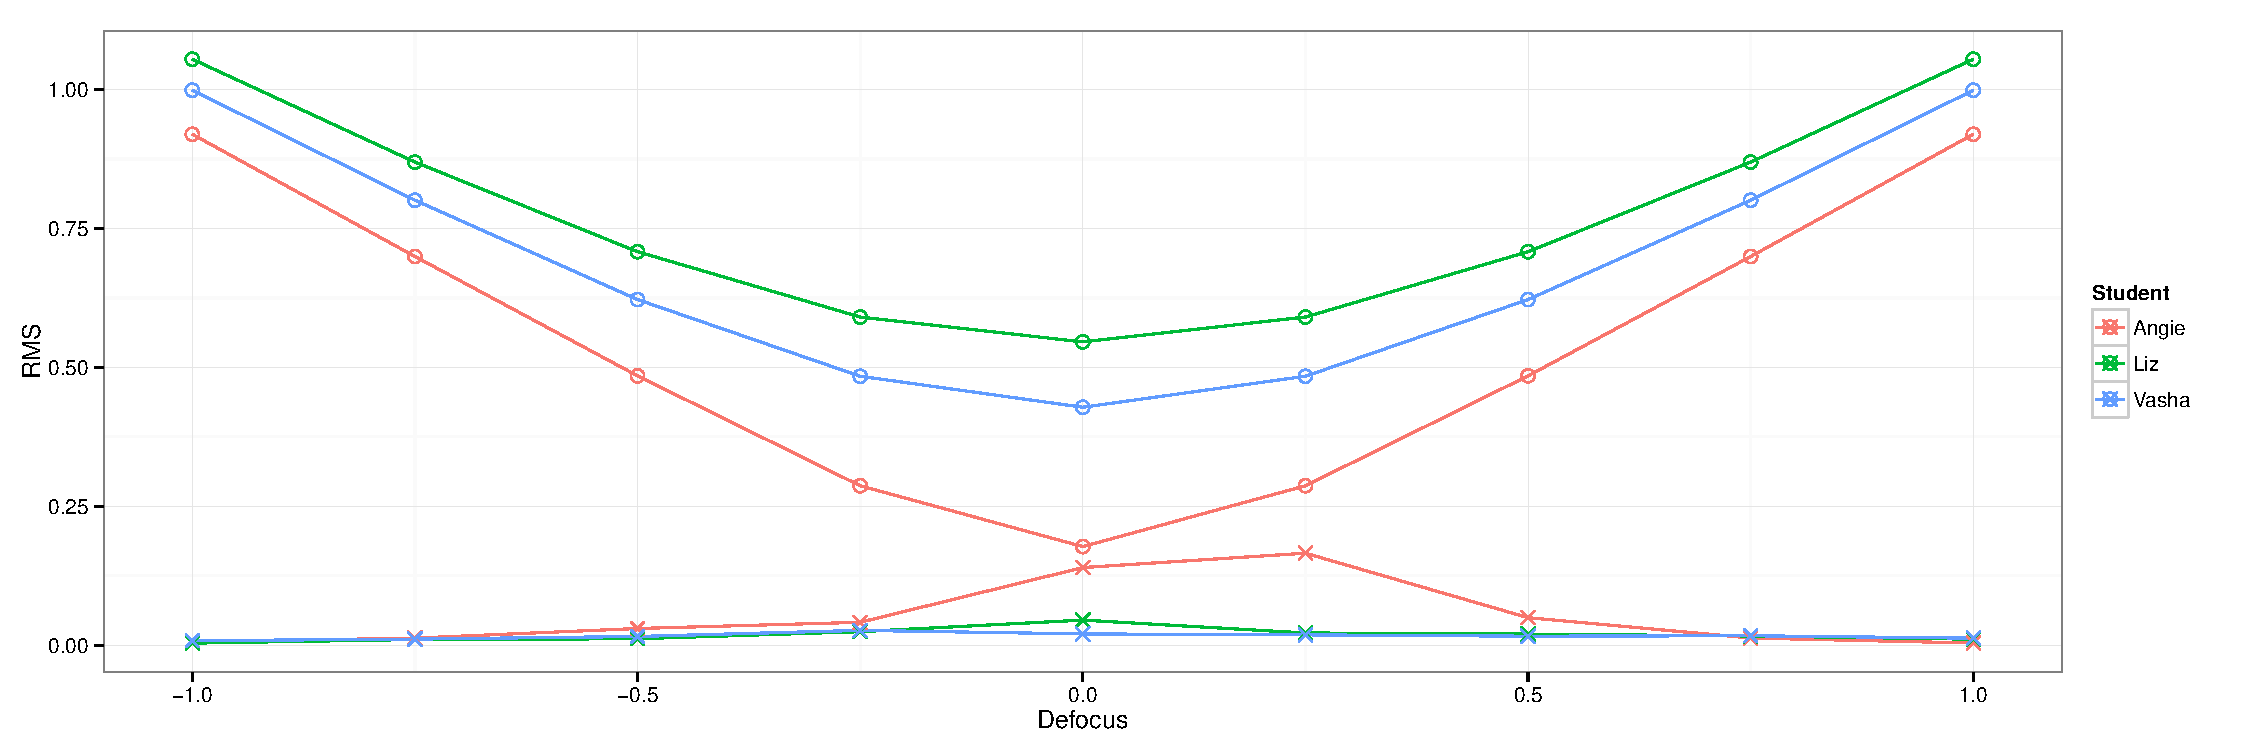
\includegraphics[width=1\linewidth]{drmsstrehl.pdf}
  \caption{RMS and Strehl values as a fucntion of defocus value for 3 students: Vasha, Angie, and Liz. Circle: Strehl Ratio, X: RMS }
  \label{fig:drmsstrehl}
\end{figure}

\clearpage

\subsubsection{PSFs for each defocus plotted above, convolved with a 20/20E}
Now, for each dfocus level, we plot the PSF, and convolve it with a 20/20E, to see the effect of each PSF on the acuity of the letter. We can then get a feel for how the aberrations from each eye cause changes in the perceived letter. This gives us another metric for visual acuity, though somewhat biased and non-objective.

+1D Defocus:
\begin{figure}[H]
\begin{subfigure}{.3\textwidth}
  \centering
  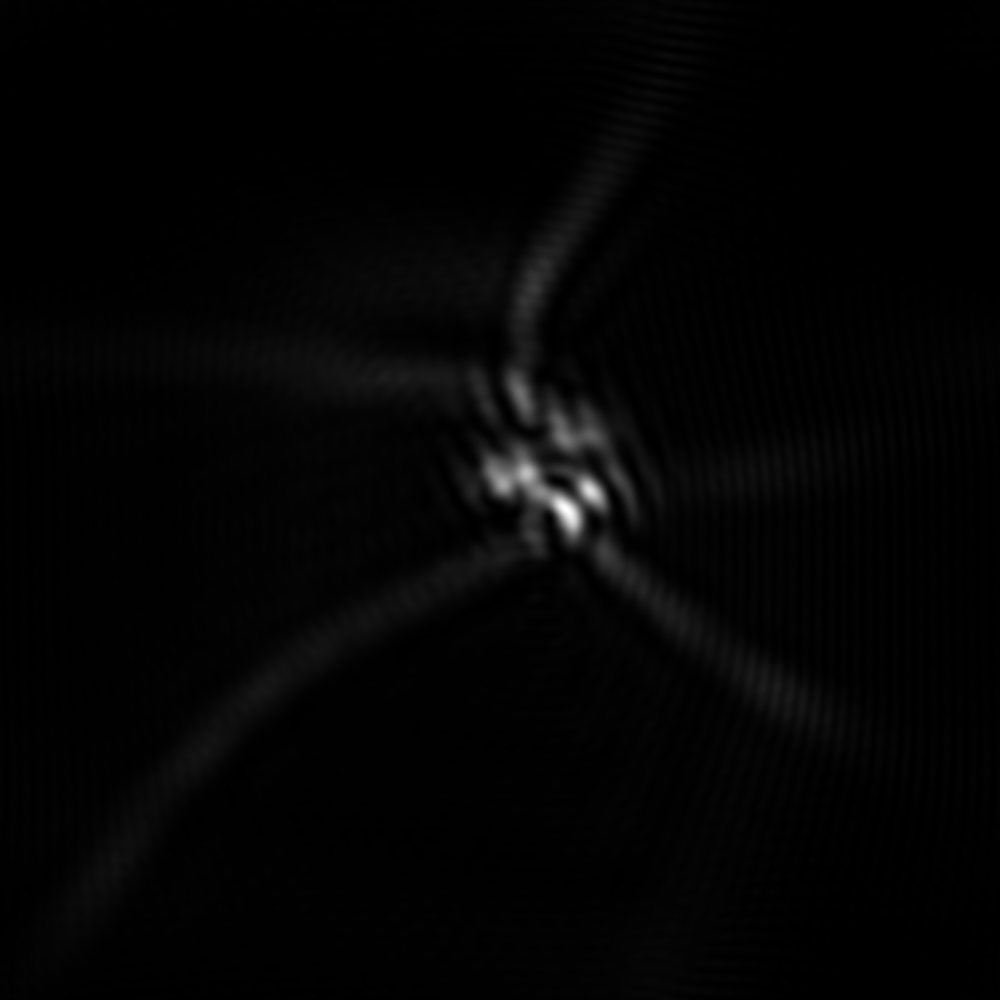
\includegraphics[width=1\linewidth]{Vasha_R_G_0530_2_500_zer_1_5_PSF.png}
  \caption{Vasha's +1D defocus PSF}
  \label{fig:vasha1dpsf}
\end{subfigure}
\begin{subfigure}{.3\textwidth}
  \centering
  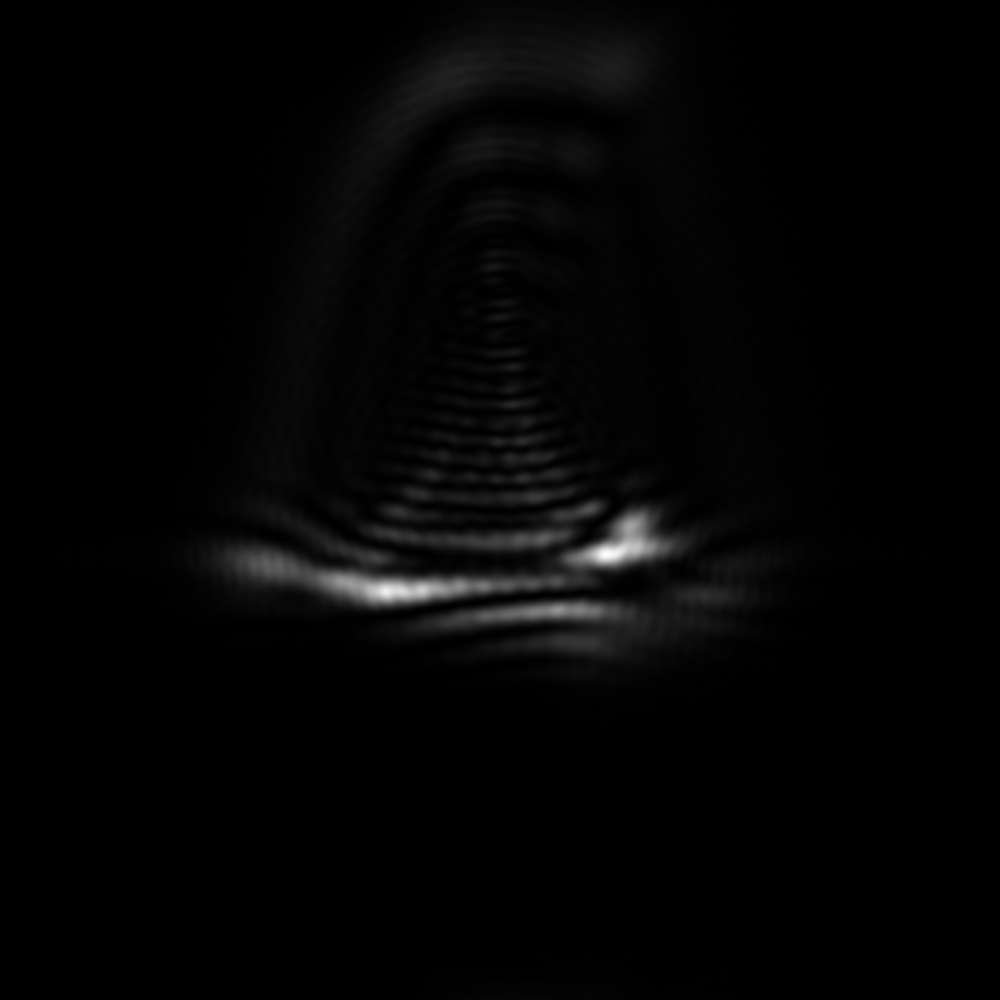
\includegraphics[width=1\linewidth]{Liz_R_G_0523_2_500_zer_1_5_PSF.png}
  \caption{Liz's +1D defocus PSF}
  \label{fig:liz1dpsf}
\end{subfigure}
\begin{subfigure}{.3\textwidth}
  \centering
  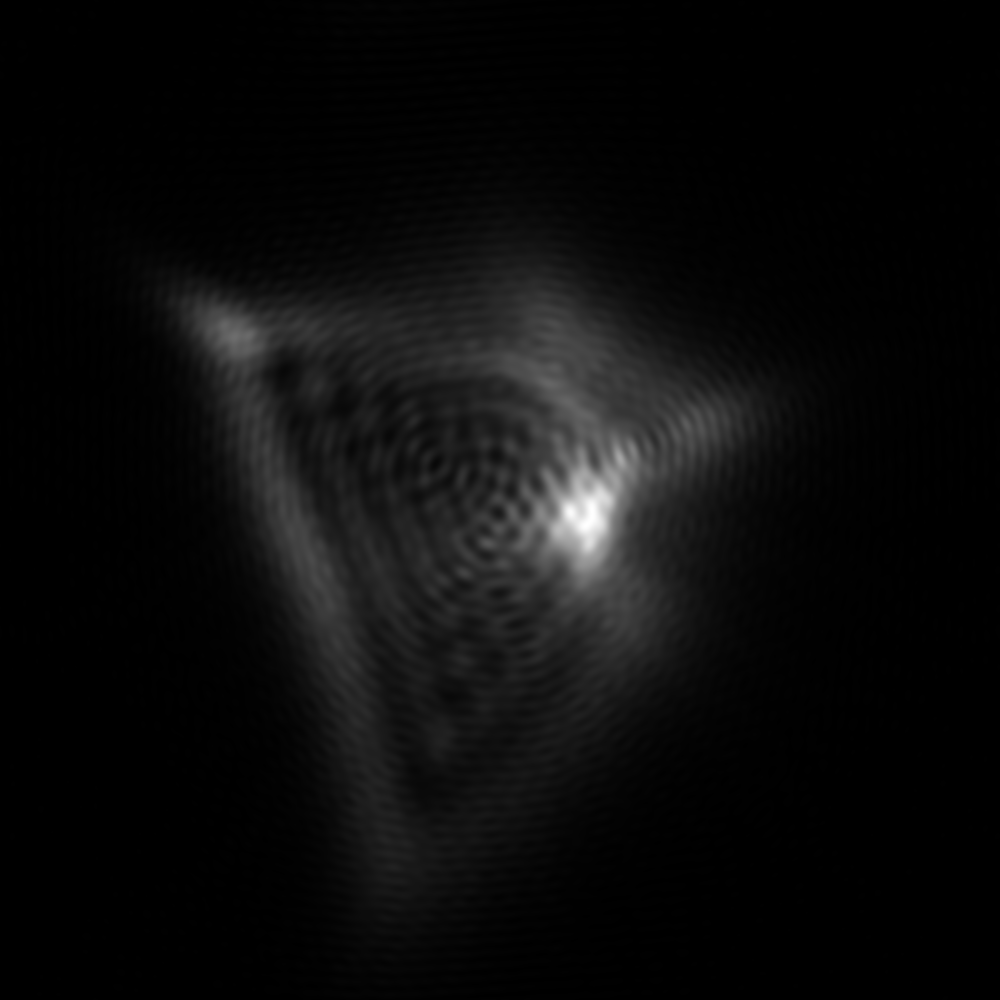
\includegraphics[width=1\linewidth]{Angie_R_0526_1_500_zer_1_5_PSF.png}
  \caption{Angie's +1D defocus PSF}
  \label{fig:angie1dpsf}
\end{subfigure}

\medskip

\begin{subfigure}{.3\textwidth}
  \centering
  
\includegraphics[width=1\linewidth]{Vasha_R_G_0530_2_500_zer_1_5_PSF_convE.png}
  \caption{Vasha's +1D Convolution}
  \label{fig:vasha1d}
\end{subfigure}
\begin{subfigure}{.3\textwidth}
  \centering
  
\includegraphics[width=1\linewidth]{Liz_R_G_0523_2_500_zer_1_5_PSF_convE.png}
  \caption{Liz's +1D Convolution}
  \label{fig:liz1d}
\end{subfigure}
\begin{subfigure}{.3\textwidth}
  \centering
  
\includegraphics[width=1\linewidth]{Angie_R_0526_1_500_zer_1_5_PSF_convE.png}
  \caption{Angie's +1D Convolution}
  \label{fig:angie1d}
\end{subfigure}
\caption{20/20 E convolved with +1D defocus PSF for 3 students}

\label{fig:Defocus_1D}
\end{figure}

\clearpage

+0.75D defocus
\begin{figure}[H]
\begin{subfigure}{.3\textwidth}
  \centering
  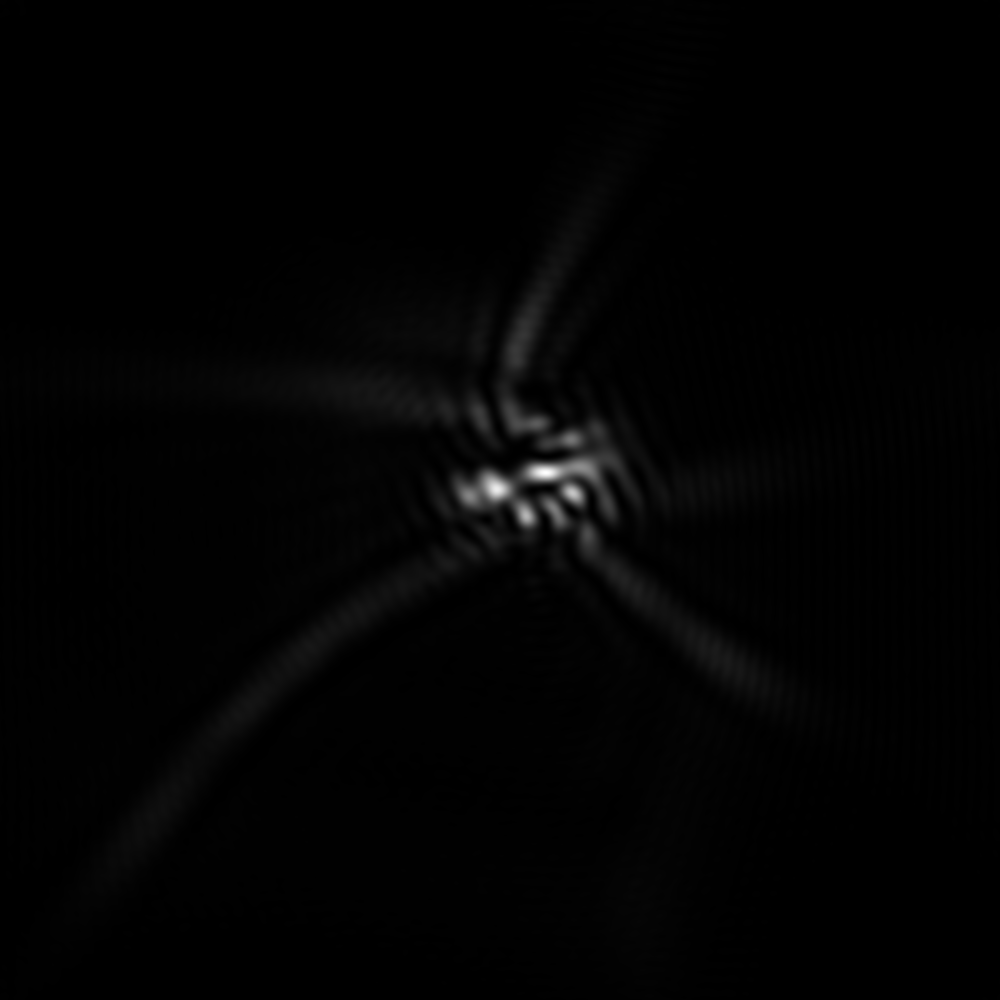
\includegraphics[width=1\linewidth]{Vasha_R_G_0530_2_500_zer_075_5_PSF.png}
  \caption{Vasha's +0.75D PSF}
  \label{fig:vasha075dpsf}
\end{subfigure}
\begin{subfigure}{.3\textwidth}
  \centering
  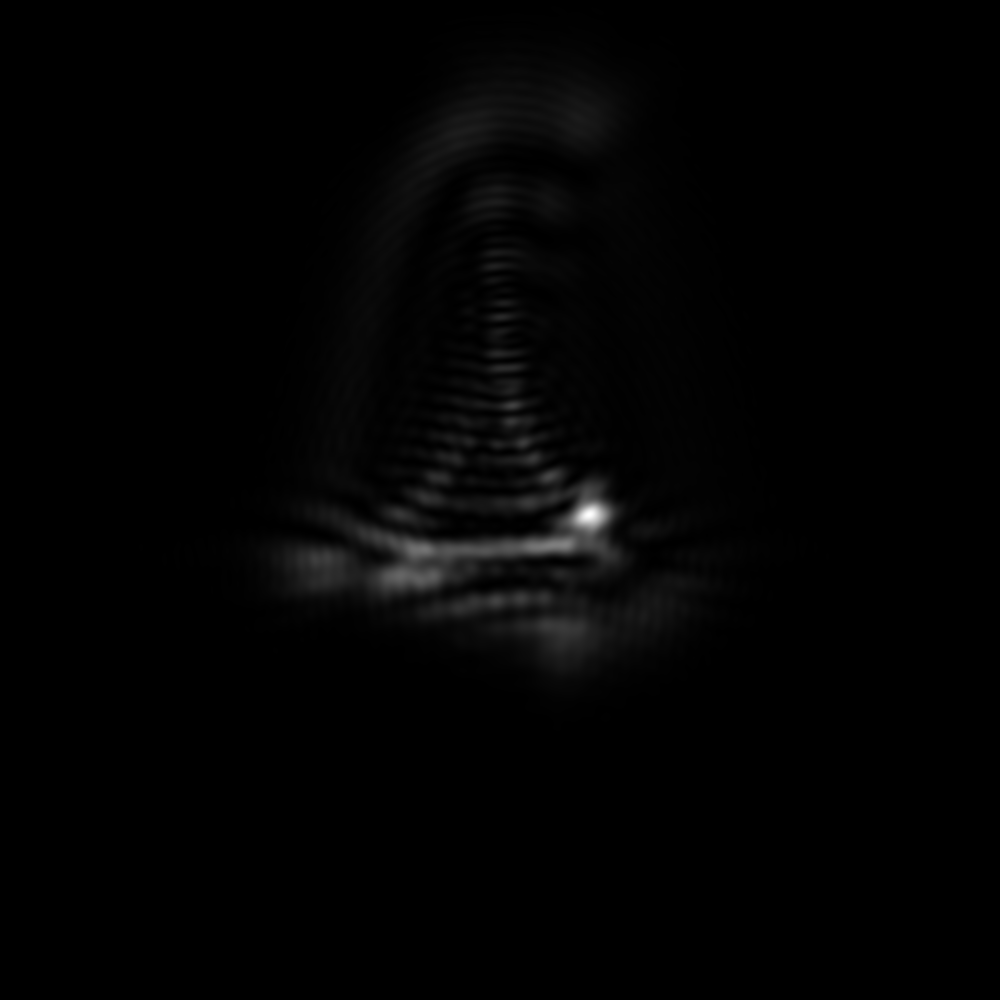
\includegraphics[width=1\linewidth]{Liz_R_G_0523_2_500_zer_075_5_PSF.png}
  \caption{Liz's +0.75D PSF}
  \label{fig:liz075dpsf}
\end{subfigure}
\begin{subfigure}{.3\textwidth}
  \centering
  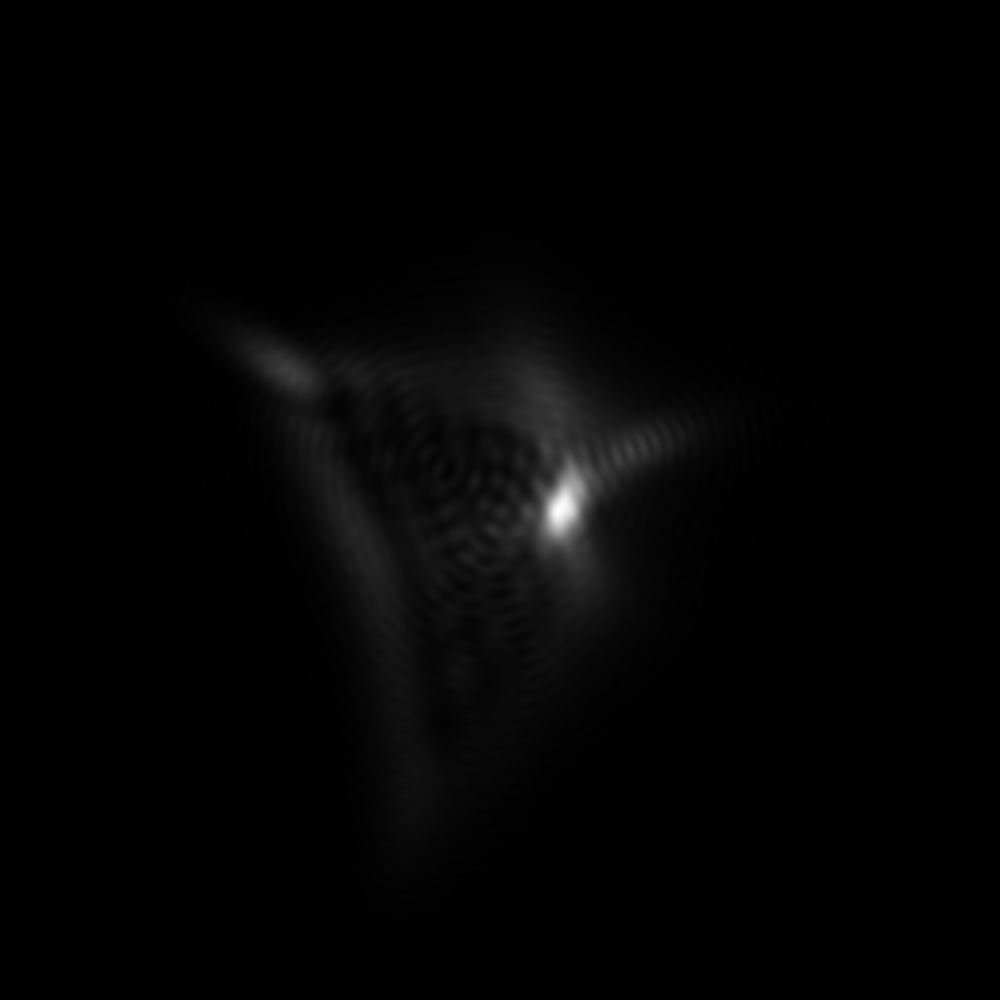
\includegraphics[width=1\linewidth]{Angie_R_0526_1_500_zer_075_5_PSF.png}
  \caption{Angie's +0.75D PSF}
  \label{fig:angie075dpsf}
\end{subfigure}

\medskip

\begin{subfigure}{.3\textwidth}
  \centering
  \includegraphics[width=1\linewidth]{Vasha_R_G_0530_2_500_zer_075_5_PSF_convE.png}
  \caption{Vasha's +0.75D Convolution}
  \label{fig:vasha075d}
\end{subfigure}
\begin{subfigure}{.3\textwidth}
  \centering
  \includegraphics[width=1\linewidth]{Liz_R_G_0523_2_500_zer_075_5_PSF_convE.png}
  \caption{Liz's +0.75D Convolution}
  \label{fig:liz075d}
\end{subfigure}
\begin{subfigure}{.3\textwidth}
  \centering
  \includegraphics[width=1\linewidth]{Angie_R_0526_1_500_zer_075_5_PSF_convE.png}
  \caption{Angie's +0.75D Convolution}
  \label{fig:angie075d}
\end{subfigure}

\caption{20/20 E convolved with +0.75D defocus PSF for 3 students}
\label{fig:Defocus_075D}
\end{figure}

\clearpage

+0.5D defocus
\begin{figure}[H]

\begin{subfigure}{.3\textwidth}
  \centering
  \includegraphics[width=1\linewidth]{Vasha_R_G_0530_2_500_zer_05_5_PSF.png}
  \caption{Vasha's +0.75D PSF}
  \label{fig:vasha05dpsf}
\end{subfigure}
\begin{subfigure}{.3\textwidth}
  \centering
  \includegraphics[width=1\linewidth]{Liz_R_G_0523_2_500_zer_05_5_PSF.png}
  \caption{Liz's +0.5D PSF}
  \label{fig:liz05dpsf}
\end{subfigure}
\begin{subfigure}{.3\textwidth}
  \centering
  \includegraphics[width=1\linewidth]{Angie_R_0526_1_500_zer_05_5_PSF.png}
  \caption{Angie's +0.5D PSF}
  \label{fig:angie05dpsf}
\end{subfigure}

\medskip

\begin{subfigure}{.3\textwidth}
  \centering
  \includegraphics[width=1\linewidth]{Vasha_R_G_0530_2_500_zer_05_5_PSF_convE.png}
  \caption{Vasha's +0.75D Convolution}
  \label{fig:vasha05d}
\end{subfigure}
\begin{subfigure}{.3\textwidth}
  \centering
  \includegraphics[width=1\linewidth]{Liz_R_G_0523_2_500_zer_05_5_PSF_convE.png}
  \caption{Liz's +0.5D Convolution}
  \label{fig:liz05d}
\end{subfigure}
\begin{subfigure}{.3\textwidth}
  \centering
  \includegraphics[width=1\linewidth]{Angie_R_0526_1_500_zer_05_5_PSF_convE.png}
  \caption{Angie's +0.5D Convolution}
  \label{fig:angie05d}
\end{subfigure}

\caption{20/20 E convolved with +0.5D defocus PSF for 3 students}
\label{fig:Defocus_05D}
\end{figure}

\clearpage

+0.25D defocus
\begin{figure}[H]

\begin{subfigure}{.3\textwidth}
  \centering
  \includegraphics[width=1\linewidth]{Vasha_R_G_0530_2_500_zer_025_5_PSF.png}
  \caption{Vasha's +0.25D PSF}
  \label{fig:vasha025dpsf}
\end{subfigure}
\begin{subfigure}{.3\textwidth}
  \centering
  \includegraphics[width=1\linewidth]{Liz_R_G_0523_2_500_zer_025_5_PSF.png}
  \caption{Liz's +0.25D PSF}
  \label{fig:liz025dpsf}
\end{subfigure}
\begin{subfigure}{.3\textwidth}
  \centering
  \includegraphics[width=1\linewidth]{Angie_R_0526_1_500_zer_025_5_PSF.png}
  \caption{Angie's +0.25D PSF}
  \label{fig:angie025dpsf}
\end{subfigure}

\medskip

\begin{subfigure}{.3\textwidth}
  \centering
  \includegraphics[width=1\linewidth]{Vasha_R_G_0530_2_500_zer_025_5_PSF_convE.png}
  \caption{Vasha's +0.25D Convolution}
  \label{fig:vasha025d}
\end{subfigure}
\begin{subfigure}{.3\textwidth}
  \centering
  \includegraphics[width=1\linewidth]{Liz_R_G_0523_2_500_zer_025_5_PSF_convE.png}
  \caption{Liz's +0.25D Convolution}
  \label{fig:liz025d}
\end{subfigure}
\begin{subfigure}{.3\textwidth}
  \centering
  \includegraphics[width=1\linewidth]{Angie_R_0526_1_500_zer_025_5_PSF_convE.png}
  \caption{Angie's +0.25D Convolution}
  \label{fig:angie025d}
\end{subfigure}

\caption{20/20 E convolved with +0.25D defocus PSF for 3 students}
\label{fig:Defocus_025D}
\end{figure}

\clearpage

0D Defocus:
\begin{figure}[H]

\begin{subfigure}{.3\textwidth}
  \centering
  \includegraphics[width=1\linewidth]{Vasha_R_G_0530_2_500_zer_0_5_PSF.png}
  \caption{Vasha's 0D PSF}
  \label{fig:vasha0dpsf}
\end{subfigure}
\begin{subfigure}{.3\textwidth}
  \centering
  \includegraphics[width=1\linewidth]{Liz_R_G_0523_2_500_zer_0_5_PSF.png}
  \caption{Liz's 0D PSF}
  \label{fig:liz0dpsf}
\end{subfigure}
\begin{subfigure}{.3\textwidth}
  \centering
  \includegraphics[width=1\linewidth]{Angie_R_0526_1_500_zer_0_5_PSF.png}
  \caption{Angie's 0D PSF}
  \label{fig:angie0dpsf}
\end{subfigure}

\medskip

\begin{subfigure}{.3\textwidth}
  \centering
  \includegraphics[width=1\linewidth]{Vasha_R_G_0530_2_500_zer_0_5_PSF_convE.png}
  \caption{Vasha's 0D Convolution}
  \label{fig:vasha0d}
\end{subfigure}
\begin{subfigure}{.3\textwidth}
  \centering
  \includegraphics[width=1\linewidth]{Liz_R_G_0523_2_500_zer_0_5_PSF_convE.png}
  \caption{Liz's 0D Convolution}
  \label{fig:liz0d}
\end{subfigure}
\begin{subfigure}{.3\textwidth}
  \centering
  \includegraphics[width=1\linewidth]{Angie_R_0526_1_500_zer_0_5_PSF_convE.png}
  \caption{Angie's 0D Convolution}
  \label{fig:angie0d}
\end{subfigure}

\caption{20/20 E convolved with 0D defocus PSF for 3 students}
\label{fig:Defocus_0D}
\end{figure}

\clearpage

-0.25D defocus
\begin{figure}[H]

\begin{subfigure}{.3\textwidth}
  \centering
  \includegraphics[width=1\linewidth]{Vasha_R_G_0530_2_500_zer_-025_5_PSF.png}
  \caption{Vasha's -0.25D PSF}
  \label{fig:vashan025dpsf}
\end{subfigure}
\begin{subfigure}{.3\textwidth}
  \centering
  \includegraphics[width=1\linewidth]{Liz_R_G_0523_2_500_zer_-025_5_PSF.png}
  \caption{Liz's -0.25D PSF}
  \label{fig:lizn025dpsf}
\end{subfigure}
\begin{subfigure}{.3\textwidth}
  \centering
  \includegraphics[width=1\linewidth]{Angie_R_0526_1_500_zer_-025_5_PSF.png}
  \caption{Angie's -0.25D PSF}
  \label{fig:angien025dpsf}
\end{subfigure}

\medskip

\begin{subfigure}{.3\textwidth}
  \centering
  \includegraphics[width=1\linewidth]{Vasha_R_G_0530_2_500_zer_-025_5_PSF_convE.png}
  \caption{Vasha's -0.25D Convolutino}
  \label{fig:vashan025d}
\end{subfigure}
\begin{subfigure}{.3\textwidth}
  \centering
  \includegraphics[width=1\linewidth]{Liz_R_G_0523_2_500_zer_-025_5_PSF_convE.png}
  \caption{Liz's -0.25D Convolution}
  \label{fig:lizn025d}
\end{subfigure}
\begin{subfigure}{.3\textwidth}
  \centering
  \includegraphics[width=1\linewidth]{Angie_R_0526_1_500_zer_-025_5_PSF_convE.png}
  \caption{Angie's -0.25D Convolution}
  \label{fig:angien025d}
\end{subfigure}

\caption{20/20 E convolved with -0.25D defocus PSF for 3 students}
\label{fig:Defocus_n025D}
\end{figure}

\clearpage


-0.5D defocus
\begin{figure}[H]

\begin{subfigure}{.3\textwidth}
  \centering
  \includegraphics[width=1\linewidth]{Vasha_R_G_0530_2_500_zer_-05_5_PSF.png}
  \caption{Vasha's -0.75D PSF}
  \label{fig:vashan05dpsf}
\end{subfigure}
\begin{subfigure}{.3\textwidth}
  \centering
  \includegraphics[width=1\linewidth]{Liz_R_G_0523_2_500_zer_-05_5_PSF.png}
  \caption{Liz's -0.5D PSF}
  \label{fig:lizn05dpsf}
\end{subfigure}
\begin{subfigure}{.3\textwidth}
  \centering
  \includegraphics[width=1\linewidth]{Angie_R_0526_1_500_zer_-05_5_PSF.png}
  \caption{Angie's -0.5D PSF}
  \label{fig:angien05dpsf}
\end{subfigure}

\medskip

\begin{subfigure}{.3\textwidth}
  \centering
  \includegraphics[width=1\linewidth]{Vasha_R_G_0530_2_500_zer_-05_5_PSF_convE.png}
  \caption{Vasha's -0.75D Convolution}
  \label{fig:vashan05d}
\end{subfigure}
\begin{subfigure}{.3\textwidth}
  \centering
  \includegraphics[width=1\linewidth]{Liz_R_G_0523_2_500_zer_-05_5_PSF_convE.png}
  \caption{Liz's -0.5D Convolution}
  \label{fig:lizn05d}
\end{subfigure}
\begin{subfigure}{.3\textwidth}
  \centering
  \includegraphics[width=1\linewidth]{Angie_R_0526_1_500_zer_-05_5_PSF_convE.png}
  \caption{Angie's -0.5D Convolution}
  \label{fig:angien05d}
\end{subfigure}

\caption{20/20 E convolved with -0.5D defocus PSF for 3 students}
\label{fig:Defocus_n05D}
\end{figure}

\clearpage

-0.75D defocus
\begin{figure}[H]

\begin{subfigure}{.3\textwidth}
  \centering
  \includegraphics[width=1\linewidth]{Vasha_R_G_0530_2_500_zer_-075_5_PSF.png}
  \caption{Vasha's -0.75D PSF}
  \label{fig:vashan075dpsf}
\end{subfigure}
\begin{subfigure}{.3\textwidth}
  \centering
  \includegraphics[width=1\linewidth]{Liz_R_G_0523_2_500_zer_-075_5_PSF.png}
  \caption{Liz's -0.75D PSF}
  \label{fig:lizn075dpsf}
\end{subfigure}
\begin{subfigure}{.3\textwidth}
  \centering
  \includegraphics[width=1\linewidth]{Angie_R_0526_1_500_zer_-075_5_PSF.png}
  \caption{Angie's -0.75D PSF}
  \label{fig:angien075dpsf}
\end{subfigure}


\medskip

\begin{subfigure}{.3\textwidth}
  \centering
  \includegraphics[width=1\linewidth]{Vasha_R_G_0530_2_500_zer_-075_5_PSF_convE.png}
  \caption{Vasha's -0.75D Convolution}
  \label{fig:vashan075d}
\end{subfigure}
\begin{subfigure}{.3\textwidth}
  \centering
  \includegraphics[width=1\linewidth]{Liz_R_G_0523_2_500_zer_-075_5_PSF_convE.png}
  \caption{Liz's -0.75D Convolution}
  \label{fig:lizn075d}
\end{subfigure}
\begin{subfigure}{.3\textwidth}
  \centering
  \includegraphics[width=1\linewidth]{Angie_R_0526_1_500_zer_-075_5_PSF_convE.png}
  \caption{Angie's -0.75D Convolution}
  \label{fig:angien075d}
\end{subfigure}

\caption{20/20 E convolved with -0.75D defocus PSF for 3 students}
\label{fig:Defocus_n075D}
\end{figure}

\clearpage

-1D Defocus:
\begin{figure}[H]

\begin{subfigure}{.3\textwidth}
  \centering
  \includegraphics[width=1\linewidth]{Vasha_R_G_0530_2_500_zer_-1_5_PSF.png}
  \caption{Vasha's -1D PSF}
  \label{fig:vashan1dpsf}
\end{subfigure}
\begin{subfigure}{.3\textwidth}
  \centering
  \includegraphics[width=1\linewidth]{Liz_R_G_0523_2_500_zer_-1_5_PSF.png}
  \caption{Liz's -1D PSF}
  \label{fig:lizn1dpsf}
\end{subfigure}
\begin{subfigure}{.3\textwidth}
  \centering
  \includegraphics[width=1\linewidth]{Angie_R_0526_1_500_zer_-1_5_PSF.png}
  \caption{Angie's -1D PSF}
  \label{fig:angien1dpsf}
\end{subfigure}

\medskip

\begin{subfigure}{.3\textwidth}
  \centering
  \includegraphics[width=1\linewidth]{Vasha_R_G_0530_2_500_zer_-1_5_PSF_convE.png}
  \caption{Vasha's -1D Convolution}
  \label{fig:vashan1d}
\end{subfigure}
\begin{subfigure}{.3\textwidth}
  \centering
  \includegraphics[width=1\linewidth]{Liz_R_G_0523_2_500_zer_-1_5_PSF_convE.png}
  \caption{Liz's -1D Convolution}
  \label{fig:lizn1d}
\end{subfigure}
\begin{subfigure}{.3\textwidth}
  \centering
  \includegraphics[width=1\linewidth]{Angie_R_0526_1_500_zer_-1_5_PSF_convE.png}
  \caption{Angie's -1D Convolution}
  \label{fig:angien1d}
\end{subfigure}

\caption{20/20 E convolved with -1D defocus PSF for 3 students}
\label{fig:Defocus_n1D}
\end{figure}

\clearpage

\subsubsection{Radial Average MTFs as a function of defocus}

Another more objective measure of visual acuity, and one with higher dimensionality, is the Radial Average MTF, where a better area under the curve for a line indicates higher acuity.

Vasha
\begin{figure}[H]
  \centering
    \includegraphics[width=1\linewidth]{vasha_dmtfs.pdf}
  \caption{Vasha's radial average MTF plot as a function of defocus}
  \label{fig:vmtfs}
\end{figure}

Liz
\begin{figure}[H]
  \centering
    \includegraphics[width=1\linewidth]{liz_dmtfs.pdf}
  \caption{Liz's radial average MTF plot as a function of defocus}
  \label{fig:lmtfs}
\end{figure}

Angie
\begin{figure}[H]
  \centering
    \includegraphics[width=1\linewidth]{angie_dmtfs.pdf}
  \caption{Angie's radial average MTF plot as a function of defocus}
  \label{fig:amtfs}
\end{figure}

\subsection{My eye at 6mm}

Now, look at differing pupil sizes in my own eye. For these calculations, return the values for defocus and astygmatism (second order ZPs), to their measured values, and add them to the calculation calculation in order to compute the defocus level that gives the highest Strehl ratio for my eye. This is then the total Strehl ratio, RMS, and MTF, rather than the High-order values.

\subsubsection{Strehl Ratio at Defocus level by Pupil Size}
Now, for each pupil size from 6 to 2 in steps of 1 mm, we find the defocus level that has the highest Strehl ratio, and plot Strehl vs pupil size.

No measurement at 2mm, so include the 6.31mm pupil measurement, and plot every 0.1D instead of 0.25D for granularity\

\begin{figure}[H]
  \centering
    \includegraphics[width=1\linewidth]{vashapupilsize.pdf}
  \caption{Vasha's Strehl Ratio as a fucntion of pupil size and defocus}
  \label{fig:amtfs}
\end{figure}

The best defocus level for each pupil size is shown in Table \ref{tab:Max Strehl for Vasha's pupil size and defocus}:

\begin{table}[htbp]
    \centering
    \begin{tabular}{lrc}\hline
        Pupil Size (mm) & Defocus (Diopters) & Strehl \\ \hline
        3 & -0.7 & 9.43$\times10^{-2}$ \\
        4 & -0.3 & 5.81$\times10^{-2}$ \\
        5 & 0 & 3.52$\times10^{-2}$ \\
        6 & 0.2 & 2.21$\times10^{-2}$ \\
        6.13 & 0.5 & 2.21$\times10^{-2}$ \\
    \end{tabular}
    \caption{Strehl vs pupil size \& defocus}
    \label{tab:Max Strehl for Vasha's pupil size and defocus}
\end{table}

As expected, the smallest pupil size has the highest Strehl ratio. This is because we are closer to a pinhole camera.

\begin{figure}[H]
  \centering
    \includegraphics[width=1\linewidth]{vashabestpupilsize.pdf}
  \caption{Vasha's Strehl Ratio as a fucntion of pupil size and defocus}
  \label{fig:amtfs}
\end{figure}

For the best Strehl ratio at any given pupil size, there is a linear relationship between the pupil size, and the defocus level which yields that Strehl ratio.

\clearpage

\subsubsection{Convolve best PSF with 20/10 letter}
Now we convolve the best PSF (highest Strehl) at each pupil size with a
20/10 letter E, and use this again to objectively measure acuity.

3mm and 4mm Pupils:
\begin{figure}[H]
\begin{subfigure}{.25\textwidth}
  \centering
  \includegraphics[width=1\linewidth]{Vasha_R_G_0530_2_300_zer_-07_3_PSF.png}
  \caption{3mm PSF}
  \label{fig:3mmStrehlpsf}
\end{subfigure}%
\begin{subfigure}{.25\textwidth}
  \centering
  \includegraphics[width=1\linewidth]{Vasha_R_G_0530_2_300_zer_-07_3_PSF_convE.png}
  \caption{3mm Convolution}
  \label{fig:3mmStrehlconv}
\end{subfigure}
\begin{subfigure}{.25\textwidth}
  \centering
  \includegraphics[width=1\linewidth]{Vasha_R_G_0530_2_400_zer_-03_4_PSF.png}
  \caption{4mm PSF}
  \label{fig:4mmStrehlpsf}
\end{subfigure}%
\begin{subfigure}{.25\textwidth}
  \centering
  \includegraphics[width=1\linewidth]{Vasha_R_G_0530_2_400_zer_-03_4_PSF_convE.png}
  \caption{4mm Convolution}
  \label{fig:4mmStrehlconv}
\end{subfigure}
\caption{Best Strehl for 3 and 4 mm Pupils}
\label{fig:3and4mmStrehl}
\end{figure}

5mm and 6mm Pupil:
\begin{figure}[H]
\begin{subfigure}{.25\textwidth}
  \centering
  \includegraphics[width=1\linewidth]{Vasha_R_G_0530_2_500_zer_0_5_PSF.png}
  \caption{5mm PSF}
  \label{fig:5mmStrehlpsf}
\end{subfigure}%
\begin{subfigure}{.25\textwidth}
  \centering
  \includegraphics[width=1\linewidth]{Vasha_R_G_0530_2_500_zer_0_5_PSF_convE.png}
  \caption{5mm Convolution}
  \label{fig:5mmStrehlconv}
\end{subfigure}
\begin{subfigure}{.25\textwidth}
  \centering
  \includegraphics[width=1\linewidth]{Vasha_R_G_0530_2_600_zer_02_6_PSF.png}
  \caption{6mm PSF}
  \label{fig:6mmStrehlpsf}
\end{subfigure}%
\begin{subfigure}{.25\textwidth}
  \centering
  \includegraphics[width=1\linewidth]{Vasha_R_G_0530_2_600_zer_02_6_PSF_convE.png}
  \caption{6mm Convolution}
  \label{fig:6mmStrehlconv}
\end{subfigure}
\caption{Best Strehl for 5 and 6 mm Pupils}
\label{fig:5and6mmStrehl}
\end{figure}

6.31mm (max size) Pupil:
\begin{figure}[H]
\begin{subfigure}{.25\textwidth}
  \centering
  \includegraphics[width=1\linewidth]{Vasha_R_G_0530_2_631_zer_05_63167_PSF.png}
  \caption{6.31mm PSF}
  \label{fig:631mmStrehlpsf}
\end{subfigure}%
\begin{subfigure}{.25\textwidth}
  \centering
  \includegraphics[width=1\linewidth]{Vasha_R_G_0530_2_631_zer_05_63167_PSF_convE.png}
  \caption{6.31mm Convolution}
  \label{fig:631mmStrehlconv}
\end{subfigure}
\caption{Best Strehl for 6.31 mm Pupil}
\label{fig:631mmStrehl}
\end{figure}


\subsubsection{MTF for best PSF}
Now we plot the radial average MTF at the defocus level that gives the highest Strehl ratio from the maximum pupil size down to 2 mm in 1 mm steps. Since there is still no 2mm pupil size, plot down to 3mm, and include the 6.13mm pupil.

6.31mm (max size) Pupil:
\begin{figure}[H]
  \centering
  \includegraphics[width=1\linewidth]{mtfvasha.pdf}
  \caption{MTF at best defocus level for each pupil size}
  \label{fig:vmtf}
\end{figure}

\section{Discussion}

\subsection{ZPs for Entire Class}

\begin{itemize}
\item Are the aberrations random? Explain your answer.

No, these aberrations are not random. It's clear that second order aberrations are the most common, with defocus, $Z_2^0$ being much larger than any other aberration. Furthermore, defocus is on average positive, while astygmatism, $Z_2^2$ was on average negative. These second order ZPs had much higher variance than any other order aberration, and 3rd order came in next. These lower order aberrations also seem to be more common than higher order, as well as having higher variance. It is not surprising really, that lower aberrations are more common, as in the spherical coordinates of the eye, they are the most simple patterns.

\item Which aberration orders are the most deleterious for vision, as quantified by
RMS?

By measure of RMS, 2nd order aberrations (defocus and astygmatism) are the most common cause of aberration in vision. 3rd and 4th order are the next most common, followed by 5th and 6th. The 2rd order aberrations also have the highest variance by far. This means that they are the most deleterious for vision as quantified by RMS, because they contribute the most to overall aberration. The 3rd order coefficients are the second highest contributors to overall aberration as measued by RMS.

\item For the 5 mm pupil, who has the highest aberration according to the Strehl ratio? According to the RMS? Are they the same?

For the 5mm pupil, according to the high order Strehl ratio, I have the most aberrated eye, followed closely by Michael. Peter and Sanam follow us. According to the high order RMS however, Liz has the most aberrated eye, then followed by me, and by Michael. These metrics do indeed give different results. The High order Strehl ratio and the total Strehl ratio however, do both rank me as the highest aberration.

\item Is the rank of image quality in the subjects the same for Strehl ratio as for RMS?

In comparing the HO-RMS and the HO-Strehl, in general the best quality (high numbers) for Strehl ratio do correspond to the best quality (low numbers) for RMS value. For example, Angie and Sylvain who have the two highest HO-Strehl ratios, also have the lowest HO-RMS values. There are however, exceptions to this. Liz for example, has by far the highest HO-RMS value, but has a HO-Strehl ratio around average for the class. Linyue also has the 3rd lowest HO-RMS value, but the 3rd highest HO-Strehl ratio.

\item Which subject has the highest image contrast image at 15 cycles per degree?

All the way from zero to 50 cycles per degree, Angie has the highest contrast image. Sylvain had an almost as high contrast image in this interval as well. Both of their image contrasts also spike again above all others in the 90-120 cycles/degree range.

\end{itemize}

\subsection{Defocus State for 3 ZPs}

\begin{itemize}
\item Does the defocus state that gives the maximum Strehl ratio match the defocus state with the minimum RMS?

For Liz and I, yes the minimum RMS and the maximum Strehl ratio defocus values match. However, for Angie, image quality as measured by Strehl is best at 0.25D defocus, while quality as measured by RMS is best at 0D defocus. 

\item Look at the convolved images as a function of defocus. In your opinion, which defocus state generates the most legible image? Comment on the relationships between legibility, Strehl ratio and RMS.

For my aberrations, the +.25D  defocus seems to be the most legible. For Liz, the +0.25 or +0.5 Diopter defocus seems to be the most legible. For Angie, it's clear that the +0.25D defocus is the most legible. This is obvious also, in looking at her PSF for this defocus, which is nearly a perfect point at this defocus.

In comparing the legibility of these letters to the calulated values for RMS and Strehl is clear that for Angie, the Strehl ratio captures true improvement in image quality, as the +0.25D PSF is the most legible. This is a strong indicator that Strehl is a better indicator of clear vision in her case, as the value for best high order Strehl ratio is at this defocus, while the 'best' (lowest) value of RMS is at 0D defocus. Interestingly, for both Liz and I, neither RMS nor Strehl ratio were good indicators of legibility given our PSFs, as both predicted 0D to be the most legible, while > +0.25D defocuses were in fact the most legible. 

Finding non-zero defocus levels to be the most legible touches on the comment Austin made in class about why we correct vision to a patients objective clarity rather than directly to correct aberrations. Because of the higher-order aberrations, these 20/20 Es are actually most clear when the image does NOT have the defocus term set to zero. A slight defocus can actually help us see more clearly, depending on the values for higher-order aberrations, which cannot be corrected with glasses or contacts.

It is interesting that Liz was given such a large value for high-order RMS, given such an average value for Strehl. Looking at her PSF, it seems she has a strong aberration in the vertical direction, and likely a relatively high value for one Z-polynomial. Checking her polynomials, indeed her value for $Z_3^{-1}$ is 0.392, a relatively large number for a high-order polynomial. Though her other coefficients are small, this leads to a large total RMS value, with a relatively normal Strehl, and a readable PSF

\item For the 5mm pupil, at what defocus state is the area under the MTF the greatest?

For me, the defocus of +0.25D has the greatest area under the curve, though 0D is a close second.

For Liz, 0D has the greatest area under the curve.

For Angie, both 0D and +0.25D have much higher areas under the curve than any other value of defocus, though +0.25D has slightly higher.

\item For the 5 mm pupil, at what defocus state is the contrast of a 30 c/deg grating the highest?

For me, +0.25D has the highest contrast for a 30 c/deg grating, though all values of defocus are very similar.

For Liz, +0.25D also has the highest contrast for a 30 c/deg grating, though again, all values of defocus are very similar.

For Angie, +0.25D is the very clear winner for this grating, though for a 15 c/deg grating would be best seen at 0D defocus.

\item Is the best focus state the same for all of the above image quality metrics?
Comment on why or why not?

These image quality metrics do give similar answers, though it seems especially in the case of Liz and I, that the two best defocus values are pretty similar, so slight differences in answers from different metrics between the two values are not surprising.

It is not all the surprising that image quality metrics do not always match legibility as seen by a person. These metrics take into account different parts of legibility, but one or the other does not determine legibility itself. RMS for example, is calculated by averaging all the coefficients for ZPs. This could mean a little bit of many aberrations, or one large aberration (like in Liz's case). While in general, many large aberrations likely means illegibility, a high RMS could correspond to many different images, and perhaps one which smears an image, but leaves is legible. A Strehl ratio, on the other hand, is calculated by looking at the maximum value for the PSF over the ideal, and is in this way a measure of how much contrast in the image. A very small Strehl ratio can guarantee illegilbility, because there is no contrast to see an image, however a given value could again correspond to many different images, some of which may be readable and not. Because an MTF is an entire function, and therefore a higher dimensional representation of aberration, it is in many ways a more informative metric than RMS or Strehl ratio. An MTF can take into account that different defocuses can be best to image different types of images (different spatial frequency) given some aberration.

\end{itemize}

\subsection{My 6.31mm Pupil}

\begin{itemize}
\item For what pupil size is the area under the MTF the greatest?

Ths 3mm pupil, with the defocus of -0.7D has the most area under the curve. This was also the puil size and defocus that had the highest Strehl ratio overall. This is not surprising, as smaller pupil size reduces aberration, with the pinhole aperture as the limit with everything in focus.

\item For what pupil size is the contrast of a 30 cyc/deg grating the highest? Based on the above results, what pupil size would provide the best acuity for each of the 3 subjects?

The 3mm pupil size also has the highest contrast at spatial frequency of 30 cy/degree. These results suggest that the smallest pupil size possible would give the highest acuity for Angie and Liz as well, regardless of the optimal level of defocus.

\item Which pupil size do you think gives the best acuity for a 20/10 letter?

Either the 3mm or 4mm pupil. The 3mm pupil convolution has the higest contrast, however the aberration in the 4mm pupil causes the image to be repeated 3 times, and therefore is easier to read because there are multiple copies.

\end{itemize}

\section{Bibliography}
\begin{thebibliography}{9}

\bibitem{hartmann1900}
  Johannes Hartmann,
  {Bemerkungen über den Bau und die Justirung von Spektrographen},
  Zeitschrift für Instrumentenkunde,
  Berlin: Julins Springer,
  20:17-27,47-58,
  1900.
  
  \bibitem{shack71}
  Roland Shack,
  {Production and use of a lenticular Hartmann screen},
  Journal of the Optical Society of America,
  Oral Presentation,
  Ramada Inn, Tucson, Arizona,
  61(5):656,
  1971.
  
\bibitem{austinsslides}
  Austin Roorda,
  {VS 212A Proseminar Optics and Dioptrics of the Eye},
  Lecture Slides  
  UC Berkeley,
  Fall, 2015.

\end{thebibliography}

\section{Other Questions}
\begin{enumerate}[1.]
\begin{item}
Describe properties of the eye that serve to reduce the effects of spherical aberration and chromatic aberration.\
\begin{itemize}
\item The eye reduces the effect of spherical aberration by keeping the eye at a small pupil size (optimal is 2-3mm) during the day when there is plenty of light available, creating a pinhole camera effect that negates aberration. The positive power of the lens also reduces the focal length, allowing for less aberration to occur before focus. Also, the combination of the positive spherical aberration in the cornea, and the negative spherical aberration in the crystalline lens, negates the total aberration when light passes through both, creating a doublet lens and resulting in a small total spherical aberration in the eye. 

\item The eye reduces the effect of chromatic aberration again by using a gradient refractive index lens, with a varied power over the lens area, caused by different ratios of protein and water, reducing effects of chromatic aberration. Also, S-cones, the cones that that are sensitive to short-wavelength light, the type of light most sensitive to focusing in front of the retina due to chromatic aberration, make up a very small portion of the fovea. Finally, the eye keeps the pupil size small during the day, when color vision is most used.

\end{itemize}

\end{item}
\begin{item}
What diameter telescope would be required to resolve two features (assume point sources) on the moon that are separated by 2 meters? \textit{Assume no atmospheric turbulence causing aberrations, image wavelength of 600 nm and a moon to earth distance of 384,400 km.}
\begin{itemize}
\item Variables:
$$d = 2m $$
$$D = 384.4\e6 m$$
$$ \lambda = 600\e{-9} m$$
$$ a = telescope diamter $$
\item Equations:
$$tan(\theta) = \frac{d}{D} $$
$$\theta_{min} = \frac{1.22*\lambda}{a} $$
\item Solve:
$$\tan(\theta) = \frac{2}{384.4\e{6}} $$
$$\theta = 5.2029\e{-9}rad $$
$$5.2029\e{-9} = \frac{1.22*600\e{-9}}{a}$$
$$a = 140.69m $$
\item Solution: The diameter of the telescope needs to be at MINIMUM 140.69 meters.
\end{itemize}

\end{item}
\begin{item}
The change in refraction of the eye as a function of wavelength is fit by the following equation (from Larry Thibos, Indiana University). $$\Delta K = 1.68524 - \frac{0.63346}{\lambda - 0.2141},$$ where $\lambda$ is the wavelength in micrometers. Using this equation, determine the placement of three different targets - one blue (440nm), one green (525nm) and one red (630 nm) - such that they are simultaneously in focus on the retina.

\begin{itemize}
\item Blue $440nm = 0.44um$
\begin{align*}
\Delta K &= 1.68524 - \frac{0.63346}{0.44 - 0.2141} \\
\Delta K &= - 1.119 \\
\end{align*}
$$K'_{eff} = K' + \Delta K$$
$$K' = \frac{n'}{k'}$$
Reduced Eye Model focused at infinity:
$$F = 60D$$ (power of eye)
$$n' = 4/3$$ (index of refraction)
$$k' = 22.22mm = 2.22E-2 $$ (axial length of eye)
\begin{align*}
k_{blue} &= \frac{1}{K} \\
k_{blue} &= \frac{1}{K'_{eff}-F} \\
k_{blue} &= \frac{1}{K'+\Delta K - F} \\
k_{blue} &= \frac{1}{\frac{n'}{k'} + \Delta K - F} \\
k_{blue} &= \frac{1}{\frac{\frac{4}{3}}{2.22E-2} -1.119 - 60} \\
k_{blue} &= \frac{1}{60 -1.119 - 60} \\
k_{blue} &= \frac{1}{-1.119} \\
k_{blue} &= -0.89365m 
\end{align*}

\item Green $525nm = 0.525um$
\begin{align*}
\Delta K_{green} &= 1.68524 - \frac{0.63346}{0.525 - 0.2141} \\
\Delta K_{green} &= - 0.352 \\
\end{align*}
(from above)
\begin{align*}
k_{green} &= \frac{1}{-0.352} \\
k_{green} &= -2.839m 
\end{align*}

\item Red $630nm = 0.630um$
\begin{align*}
\Delta K_{red} &= 1.68524 - \frac{0.63346}{0.63 - 0.2141} \\
\Delta K_{red} &= 0.162
\end{align*}
(from above)
\begin{align*}
k_{red} &= \frac{1}{0.162} \\
k_{red} &= 6.169m
\end{align*}

\item These values seem a bit fishy since this would cause yellow light at $\Lambda = 589nm$ to have a $\Delta K$ of zero, and therefore $k = \infty$, when the value should be zero for this light, as it's the normalization. Furthermore, it seems strange that the order of short to long wavelength light is not respected in the values for placement in front of and behind the target. Perhaps this is an artifact of focusing at infinity (as it really doesn't make sense to put a target 6 meters behind or in front of infinity) Maybe this is a special case for the relationship between the target, and we could solve at a given value of focus such as setting $k_{yellow} = 1m$.

\end{itemize}

\end{item}
\end{enumerate}

\end{document}